% TODO: Do I mention $K = 50$ somewhere?
\documentclass[
        a4paper,
        titlepage,
        twoside,
        parskip,
        numbers=noenddot
        ]{scrbook}
\setlength{\parskip}{6pt}
\setlength{\parindent}{15pt}

\usepackage[table,usenames]{xcolor}
\definecolor{darkred}{rgb}{0.5,0,0}
\definecolor{darkgreen}{rgb}{0,0.4,0}
\definecolor{darkblue}{rgb}{0,0,0.5}

% \usepackage{layouts} printinunitsof
\usepackage{amsmath}
\usepackage{amssymb}
\usepackage{algorithm}
\usepackage[noend]{algpseudocode}
% \usepackage{hyperref}
\usepackage[utf8]{inputenc}
\usepackage{pifont}
\usepackage{booktabs}
\newcommand{\ra}[1]{\renewcommand{\arraystretch}{#1}}
\usepackage{textcomp}
\newcommand{\cmark}{\ding{51}}
\newcommand{\xmark}{\ding{55}}
\newcommand{\specialcell}[2][c]{%
   \begin{tabular}[#1]{@{}c@{}}#2\end{tabular}}

\usepackage{textcomp,amsmath}     % Mathezeichen etc.
\usepackage{graphicx}             % Graphiken einbinden
\usepackage{makecell}
\usepackage{soul}
\usepackage{ulem, xpatch}
\normalem
\xpatchcmd{\sout}
  {\bgroup}
    {\bgroup\def\ULthickness{1.1pt}}
      {}{}

\graphicspath{{./figures/}}
\DeclareGraphicsExtensions{.pdf,.png,.jpg}
\usepackage{rotating}
\usepackage[labelsep=colon]{caption}
\usepackage{subcaption}
\usepackage{threeparttable}

% bibtex
\usepackage{url}
\usepackage[backend=bibtex, style=numeric]{biblatex}

\bibliography{library}

\usepackage{chngcntr}
\usepackage{paralist}
% \usepackage{bold-extra}
\usepackage{tabularx}
\usepackage{tabulary}
\usepackage{multicol}
\usepackage{multirow}
% \usepackage{tcolorbox}% http://ctan.org/pkg/tcolorbox
\usepackage{framed}
\newcommand{\topicbox}[1]{
  \setlength{\OuterFrameSep}{0pt}
  \begin{framed}
    #1
  \end{framed}
}
\newcommand{\topicboxList}[1]{
  \setlength{\OuterFrameSep}{0pt}
  \newline
  \begin{minipage}{\linewidth}
    \vspace{6pt}
    \begin{framed}
      #1
    \end{framed}
    \vspace{6pt}
  \end{minipage}
}
\usepackage{listings}
\usepackage[toc,page]{appendix}
\usepackage{hyperref}
\hypersetup{
  colorlinks=true,
  citecolor=darkgreen,
  linkcolor=darkred,
  urlcolor=darkblue,
  filecolor=red,
  pdftitle={Master's Thesis},
  pdfauthor={Stefan Bunk},
  pdfpagemode={UseNone}
}
\usepackage{cleveref}
\usepackage{varwidth}
\DeclareCaptionFormat{centerformat}{%
  % #1: label (e.g. "Table 1")
  % #2: separator (e.g. ": ")
  % #3: caption text
  \begin{varwidth}{\linewidth}%
    \centering
    #1#2#3%
  \end{varwidth}%
}
\captionsetup{format=centerformat}% global activation

\renewcommand\theadfont{\bfseries}
\newcommand*{\tsubhead}[1]{\itshape #1}

\usepackage{amsthm}
\newtheorem{keyexmp}{Keyword Example}[section]

\newtheoremstyle{break}%
{}{}%
{\itshape}{}%
{\bfseries}{}% % Note that final punctuation is omitted.
{\newline}{}
\theoremstyle{break}
\newtheorem{exmp}{Example}[section]
\crefname{exmp}{Example}{Examples}

%\newenvironment{fexmp}
%  {\begin{mdframed}\begin{exmp}}
%  {\end{exmp}\end{mdframed}}

% Make a | to a | surrounded by spaces
\newcommand{\spacedpipe}{\ |\ }
\DeclareMathOperator*{\argmin}{arg\,min}
\DeclareMathOperator*{\argmax}{arg\,max}

\titlehead{

\includegraphics{figures/hpi_logo_cmyk_wb_sl2}
}
\subject{Master's Thesis}
\title{Improving Probabilistic Topic Models using Word Embeddings
\\ \bigskip
% http://www.duden.de/sprachwissen/sprachratgeber/schreibung-von-fremdwoertern-aus-dem-englischen
\large{Verbessern probabilistischer Topic-Modelle mithilfe von Vektorrepräsentationen von Wörtern}}
\author{Stefan Bunk\\{\small{\url{stefan.bunk@student.hpi.uni-potsdam.de}}}}
\date{December 23rd, 2016}
\publishers{
Information Systems Group \\
Hasso-Plattner-Institute, Potsdam, Germany \\ \vspace{1cm}
Supervisor: Dr. Ralf Krestel}

\pagestyle{headings}
\makeatletter
\def\BState{\State\hskip-\ALG@thistlm}
\makeatother

\begin{document}
% \frontmatter
\maketitle
\cleardoublepage

\makeatletter
\@openrightfalse

\chapter*{Abstract}
Probabilistic topic models, especially Latent Dirichlet Allocation (LDA), have proved to be powerful for detecting hidden topics in large text collections.
Recently, word embedding methods have gained popularity for language modeling.
Because of the different background of both methods, few work exists, which uses.

% Given a collection of documents, LDA finds hidden themes
useful for discovering latent topics in large text collections.

We propose WELDA, a new topic model, which uses word embeddings to improve the topic coherence.
We extensively evaluate WELDA and compare it with competitive approaches.
WELDA outperforms other models on topic coherence, while at the same time keeping acceptable performance in document classification.


\chapter*{Zusammenfassung}
Abstract Deutsch

\@openrighttrue
\makeatother

% TODO: Remove
\setcounter{secnumdepth}{4}
\setcounter{tocdepth}{4}
\tableofcontents
% \mainmatter

\chapter{Introduction}
\label{sec:introduction}
% \begin{algorithm}
%   \caption{Gibbs sampling in LDA}
%   \label{alg:welda_init}
%   \begin{algorithmic}[1]
%     \Procedure{GibbsSampling}{set of documents}
%     \State{Randomly initialize words to topics}
%     \For{iteration i}
%       \For{document d}
%         \For{word w in document d}
%           \State{Calculate distribution over topics for word w}
%           \State{Sample new topic for word w}
%           \State{Update counts}
%         \EndFor
%       \EndFor
%     \EndFor
%     \EndProcedure
%   \end{algorithmic}
% \end{algorithm}
% \begin{equation*}
%   p(z_w = t | Z) \propto (N_{d}^{t} + \alpha) *  \frac{N^{t, w} + \beta}{N^{t} + V * \beta}
% \end{equation*}
% \begin{algorithm}
%   \caption{Gibbs sampling in WELDA}
%   \label{alg:welda_init}
%   \begin{algorithmic}[1]
%     \Procedure{GibbsSamplingWELDA}{set of documents}
%     \State{Run LDA as initialization step}
%     \For{iteration i}
%       \State{Estimate distribution parameters for all topics independently}
%       \For{document d}
%         \For{word w in document d}
%           \State{Calculate distribution over topics for word w}
%           \State{new\_topic\_id $\gets$ Sample new topic for word w}
%           \If{coin\_flip($\lambda$)}
%             \State{sample $\gets$ Sample from distribution of $new\_topic\_id$}
%             \State{w $\gets$ Find nearest word for $sample$}
%           \EndIf
%           \State{Update counts}
%         \EndFor
%       \EndFor
%     \EndFor
%     \EndProcedure
%   \end{algorithmic}
% \end{algorithm}

A core task in natural language processing (NLP) is to understand the meaning of words.
Many downstream NLP tasks benefit from this, for example, text categorization, part-of-speech tagging and machine translation.
A popular concept to quantify the meaning of a word is to look at the contexts in which the word appears.
A famous quote by Firth says: ``You shall know a word by the company it keeps''~\cite{Firth1957}.
In other words, if two words occur in similar contexts, they are similar.
This assumption, also known as the distributional hypothesis, has driven the development of many models for text.

Two of these models are topic models and word embeddings, which we will focus on in this thesis.
Topic modeling tries to reconstruct the topics in a collection of text with an unsupervised learning approach.
It assumes that an author has certain topics in mind when writing a document, which are chosen before any documents are written.
For example, an author could decide to write a document about \emph{politics} (70~\%) in \emph{sports} (30~\%) and then picks the words ``coalition'', ``election'' and ``corruption'' for \emph{politics} and the words ``soccer'' and ``ball'' for \emph{sports}.
Topic modeling techniques try to recover the hidden topics in large corpora, i.e.\ find out that ``soccer'' and ``ball'' come from the same topic.
The state of the art is Latent Dirichlet Allocation (LDA) by Blei et al.~\cite{Blei2003}.
Topic models are probabilistic models, which means they provide probability distributions as the result.
Therefore, the topics can be easily interpreted by humans.
Topic models have several applications, mostly in information retrieval, where they can help navigate large corpora or augment search queries.
Topic models have also been applied in bioinformatics, where they help understand evolution~\cite{Pritchard2000}.

The idea of word embeddings is to assign each word in a vocabulary a vector in a high-dimensional vector space.
This vector representation of the word is called the embedding of the word.
Typically, the vector space contains $50$ to $600$ dimensions~\cite{Mikolov2013}.
The word embeddings are learned automatically using neural networks.
Although the idea is quite old~\cite{Bengio2003,Rumelhart1988}, the method has recently gained a lot of popularity in the research community~\cite{Levy2014,Levy2014a,Mikolov2013b}.
This is because of performance improvements of CPUs and GPUs and because of better training algorithms, which made training these models on huge amounts of data feasible in recent years.
Especially the work of Mikolov et al.~\cite{Mikolov2013b,Mikolov2013,Mikolov2013a} and the publication of the open-source tool \emph{word2vec}, which allows to train on billions of words in a realistic time frame, must be mentioned.
The training in word2vec works in a supervised manner.
A sliding window runs over the text and each word must try to predict its surrounding words.
This way, the context of a word is encoded in the vector representation of a word.
Using a clever network architecture and by training on many samples, these vectors exhibit interesting properties.
First, similar words tend to be in similar positions in the vector space.
For example, when looking for the most similar words for ``France'' using cosine distance, the model outputs ``Spain'', ``Belgium'', ``Netherlands'' and ``Italy''.
Second, the word vectors exhibit interesting linear relationships.
For example, when calculating the vector $\vec{v}_{king} - \vec{v}_{man} + \vec{v}_{woman}$ and looking for the closest word to the vector result, the result is the word ``queen''~\cite{Mikolov2013b}.

\section{Motivation}
The two approaches have different origins.
Word embeddings have their roots in the neural network and deep learning community, while topic modeling stems from Bayesian statistics, which is why traditionally there is not much research combining the two methods.
In this master thesis, we aim to explore potential synergies between these technologies.
Combining the two methods is a promising direction for research, because of several reasons:
First, the two models capture different notions of similarity: the word-based embedding models focus on semantic similarity, e.g. ``lecturer'' and ``teacher'', while the document-based topic models capture relatedness, e.g. ``teacher'' and ``school''.
Second, word2vec can be trained on much larger corpora than topic models, thereby allowing more semantic information to be used during the topic model inference.
Third, word embeddings lack human interpretability, which is where the probabilistic view of topic models can help.
In particular, it might be useful to investigate Baroni's question ``whether the two types of models are complementary in the errors they make, in which case combined models could be an interesting avenue for future work''~\cite{Baroni2014}.
In general, there are two ways of combining these two methods: one can create better topic models or one can create better word embeddings.
In this thesis, we focus on the former.

We illustrate in Figure~\ref{fig:figure1} how word embeddings can help to improve topic models.
The figure shows a section of a word embedding space, which we projected down to two dimensions via principal component analysis.
The words marked by black crosses and by the red minuses form the top ten words of a topic learned by LDA.
They grey dots in the background represent other words in the embedding space.
If one plots a probability distribution for the words in the embedding space (grey isolines), it is noticeable, that the words with the lowest probabilities are also the words which fit the least into the topic (the words ``one'', ``question'' and ``claim'').
The topic could be improved by picking words in the embedding space, which are close to the existing words in the topic.
In the figure, we illustrated this with the words ``existence'', ``faith'' and ``life'', which form a stronger topic with the rest of the words.
We want to build a model, which leverages this information from the embedding space to create better topics.

\counterwithout{figure}{chapter}
\begin{figure}
       \centering
       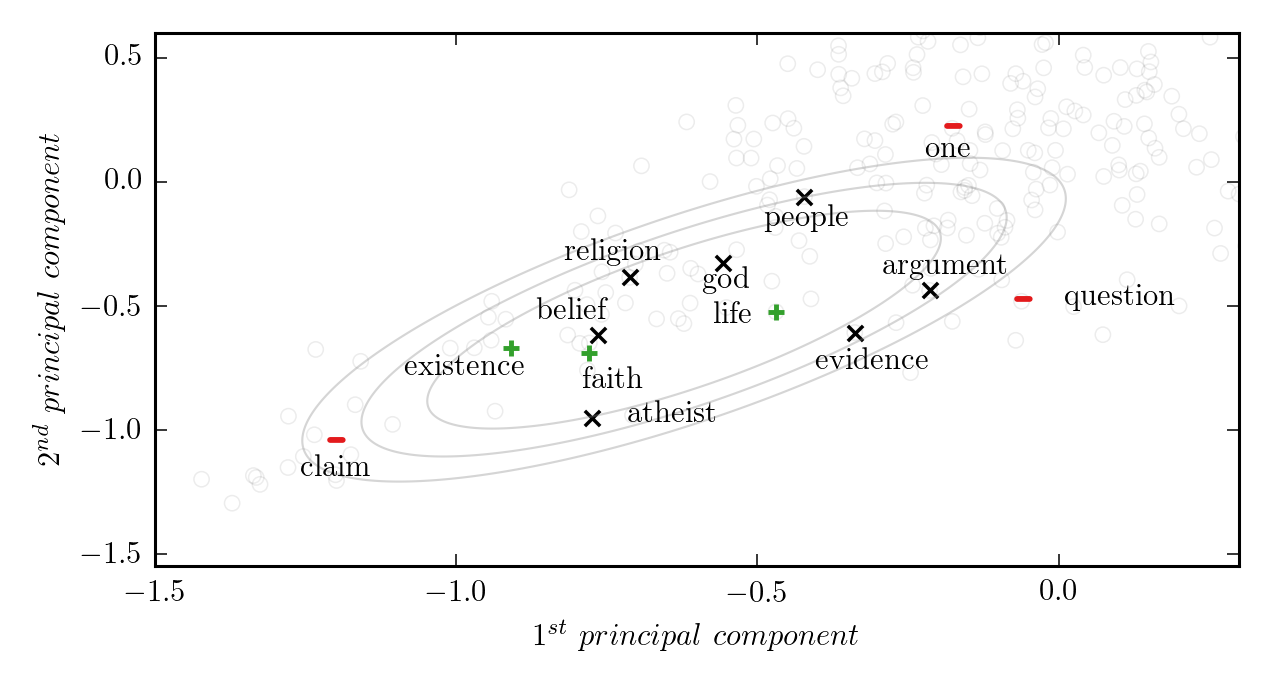
\includegraphics[width=\textwidth]{figures/figure1.png}
       \caption{Illustration of an LDA topic in the word embedding space, which we projected down to two dimensions.
       % The grey isolines show a probability distribution learned from the words.
       By picking new words (green pluses) close to the existing words in the embedding space, weaker words (red minuses) can be removed from the topic. This process makes the topic more helpful and easier understandable.}
       \label{fig:figure1}
\end{figure}
\counterwithin{figure}{chapter}

\section{Contributions}
The contributions of this thesis are:
\begin{itemize}
  \item
    We propose a new topic model called WELDA (Word Embedding LDA).
    WELDA learns a multivariate topic distribution for each topic in the embedding space.
    This distribution is then used to sample new, similar words for existing topics, thus improving the topics.
    We will present the full inference algorithm, discuss the implementation details and thoroughly evaluate WELDA.
  \item
    Recently, there has been a lot of research on combining topic models and word embeddings for improved topic models~\cite{Batmanghelich2016,Das2015,Li2016,Nguyen2015} .
    We run an exhaustive evaluation of these models and WELDA on two tasks.
    The first, topic coherence, evaluates the top words in a topic with respect to interpretability by humans, i.e. how helpful and understandable are the topics.
    The second task, document classification, uses the topic model output for text classification.
    To complete the evaluation, we also ran a manual evaluation on the word intrusion task~\cite{Chang2009}.
  \item
    We demonstrate the usefulness of word embeddings trained on small corpora, when training topic models.
    In general, word embeddings need huge amounts of training data to be accurate.
    However, when evaluating embeddings with respect to typical topic model metrics like topic coherence or document classification, embeddings trained on the small corpora itself can be superior.
\end{itemize}

\section{Structure}
This master thesis is structured as follows:

\noindent Chapter~\ref{sec:related_work} shows related work.
We will introduce topic models and word embeddings and show how they are trained.
We will then compare the two techniques and present existing combinations of both.

\noindent In Chapter~\ref{sec:welda}, we will present the WELDA algorithm.
We will discuss different choices of topic distributions -- Gaussian distributions, von Mises-Fisher distributions and Gaussian mixtures -- as well as important implementation details, such as the necessary nearest-neighbour search, the background topic and why we run LDA first.

\noindent Chapter~\ref{sec:welda_discussion} will present our analysis of WELDA on two common text corpora: \textsc{20News} and \textsc{Nips}.
We will determine good parameter settings for both topic coherence and document classification.

\noindent Chapter~\ref{sec:comparative_evaluation} will present a comparison of WELDA against other topic models techniques, which are enhanced by word embeddings.
Concretely, we will compare against TopicVec by Li et al.~\cite{Li2016}, Gaussian LDA by Das et al.~\cite{Das2015}, Latent Feature Topic Models by Nguyen et al.~\cite{Nguyen2015} and spherical topic modeling by Batmanghelich et al.~\cite{Batmanghelich2016}.
We will also present the results of our manual word intrusion study we conducted to evaluate the different models.
In this task, participants were asked to detect a wrong word hidden in the top words of a topic.

\noindent Finally, in Chapter~\ref{sec:conclusion} we conclude our work with our results and give an outlook to future work.

\chapter{Related work}
\label{sec:related_work}
In this section we will present topic models and word embeddings.
We will show their model, how they are trained and how they are evaluated.
We will end with a comparison of the two models and existing combinations between these two models.

\section{Topic modeling}
Many methods for modeling natural language text have been proposed.
An early popular method was the tf-idf~\cite{SparckJones1972} scheme.
This method represents a document with the counts of the terms occuring the document (tf: term frequency).
The counts are normalized by the number of documents a term occurs in the corpus (idf: inverse document frequency).
A high value in tf-idf is reached, when a word occurs in a document often, but only in a few documents in the entire collection at all.
When applying this method to an entire corpus, this method forms a large matrix with the rows representing the documents, the columns representing the words and the cells containing the tf-idf values.
Later, latent semantic analysis (LSA)~\cite{Deerwester1990} was proposed to reduce this large matrix to a smaller subspace using singular value decomposition.
This can capture ``some aspects of linguistic notions such as polysemy and synonymy''~\cite{Blei2003}.

While these approaches have their origins in linear algebra, topic models have been developed from a probabilistic view to allow better interpretation.
Topic models are generative probabilistic models of a document collection, which assume hidden topics have guided the generation of the text.
In this way of thinking, an author picks certain topics to write about and then picks words associated with these topics for a specific document.
The goal is then to uncover the unseen, so called ``latent'', topics from a text corpus.
All of these approaches have in common that they assume a bag-of-words representation of documents, i.e. the order of the words in the document is discarded.

\subsection{Early approaches}
A basic generative topic model is the mixture of unigrams model~\cite{Nigam2000}.
In this model, a topic is a fixed probability distribution over the vocabulary.
A document is created by choosing a topic and then picking words from this topic.
However, this method allows only one topic per document, which limits its predictive power.
Also, some documents inherently contain more than one topic, imagine for example a document about ``corruption in football'', which will contain words from a \emph{politics} as well as a \emph{sports} topic.

A more sophisticated topic model is probabilistic latent semantic analysis (pLSA) by Hofmann~\cite{Hofmann1999}, which allows multiple topics per document.
The model is fitted with an expectation-maximization algorithm.
However, pLSA does not provide a full generative model applicable to unseen documents.
Also, as the number of parameters grows linearly with the number of training documents, it tends to overfit~\cite{Blei2003}.

\subsection{Latent Dirichlet allocation (LDA)}

\begin{figure}
       \centering
       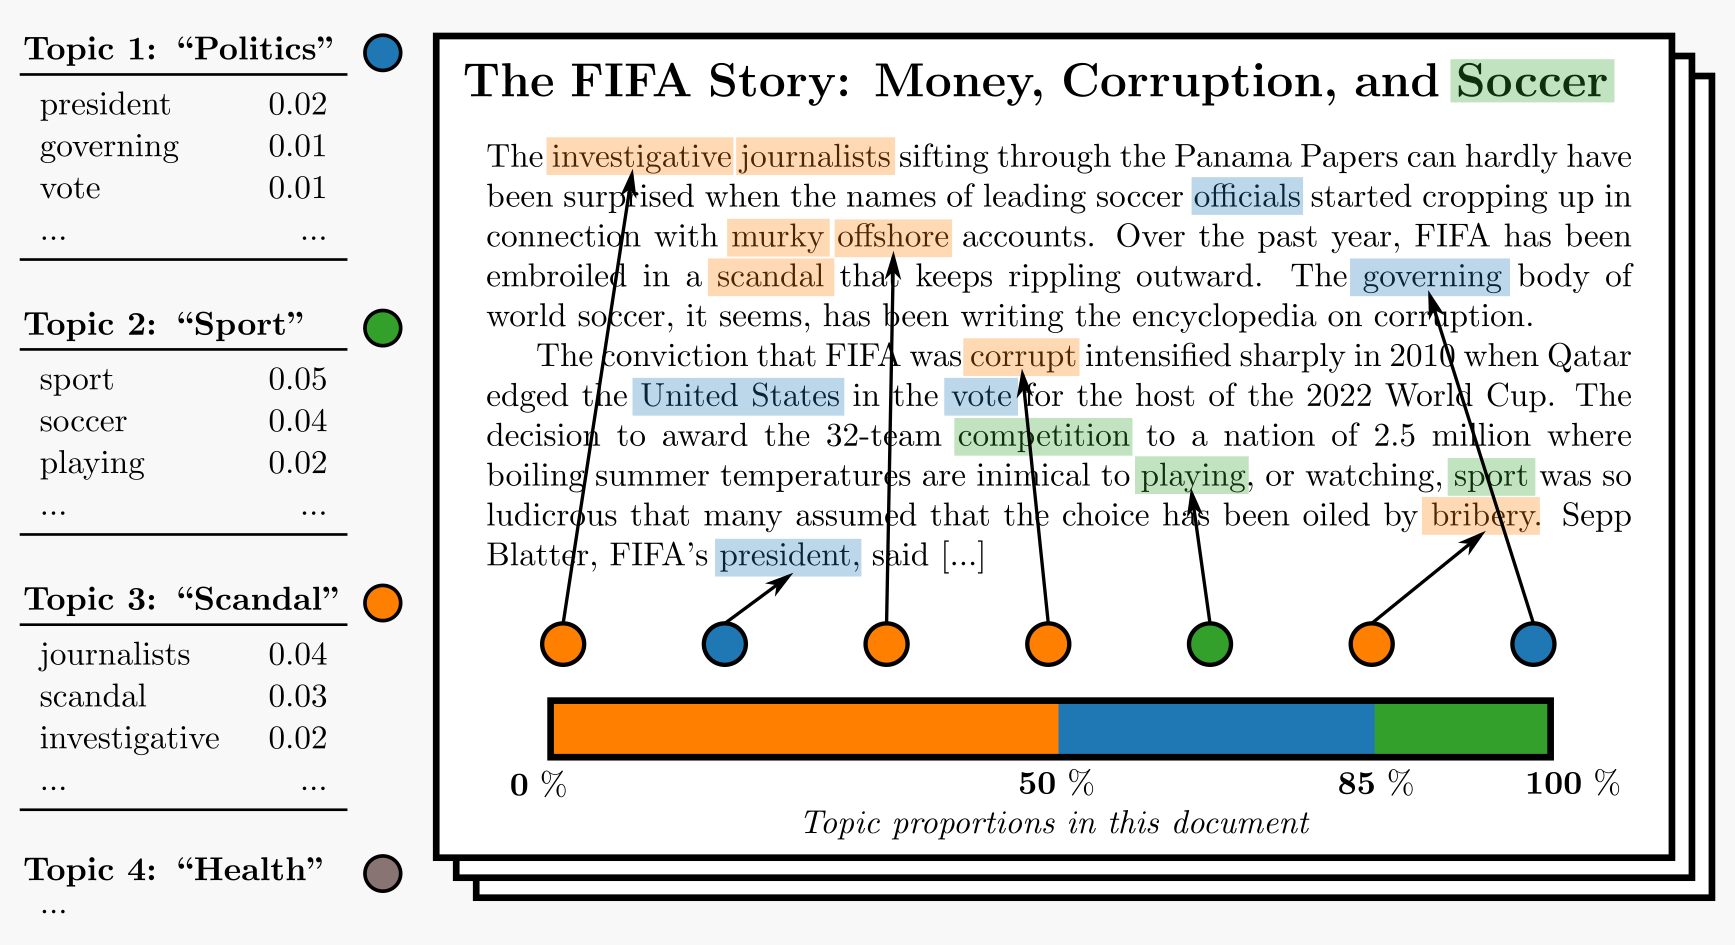
\includegraphics[width=\textwidth]{figures/lda_showcase.pdf}
       \caption{Illustration of the generative model of LDA: At first, the topic proportions for each document are generated (bottom).
       Then the topics are sampled from this multinomial distribution.
       Afterwards, the actual words are sampled depending on the topics and the word distributions of these topics (left).
       Note that in reality every word has a topic and that the topics do not have a title.}
       \label{fig:lda_showcase}
\end{figure}

LDA was proposed by Blei et al.~\cite{Blei2003} for modeling text corpora and other collections of discrete data.
It is an unsupervised algorithm, which provides a full generative model for documents.
It can automatically detect similarities between words and group them in one topic.
The number of topics $K$ is fixed for the model and must be chosen beforehand.
LDA defines a topic as a distribution over a fixed vocabulary.
Different topics assign different probabilities to the same word, for example, the word ``soccer'' would have a much higher probability in a \emph{sports} topic than in a \emph{politics} topics.
The opposite would hold for the word ``president''.
Note that a topic is only a distribution over words, i.e.\ LDA does not generate a name or a summary for a topic.

\begin{figure}
       \centering
       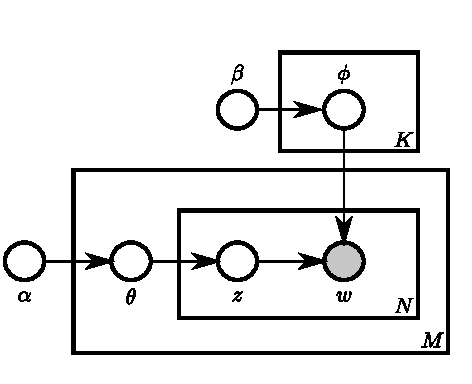
\includegraphics{figures/lda.pdf}
       \caption{Graphical model for latent Dirichlet allocation with $K$ topics, $M$ documents and $N$ words in a document.}
       \label{fig:lda}
\end{figure}

We illustrate the intuition behind LDA in Figure~\ref{fig:lda_showcase}\footnote{Article in the figure taken from \\ \url{http://www.worldpolicy.org/blog/2016/04/27/fifa-story-money-corruption-and-soccer}}.
In LDA, a document is assumed to consist of one or several topics with a fixed multinomial word distribution.
A document could be $20~\%$ about \emph{sports} and $80~\%$ percents about \emph{politics}, or $30~\%$ about \emph{climate}, $25~\%$ about \emph{cars} and $45~\%$ about \emph{politics}.
In general, LDA aims to generate sparse distributions for both cases, i.e.\ a topic should have only a few words (relative to the vocabulary of the entire corpus) with high probability and a document should have only a few topics.
The sparsity is governed by two scalar hyperparameters $\alpha$ and $\beta$, which influence two symmetrical prior Dirichlet distributions:
$\alpha$ influences the document-topic distributions and $\beta$ influences the topic-word distributions.

With these two hyperparameters, the generative document creation process of LDA can be summarized as follows:
\begin{enumerate}
       \item Fix number of topics $K$ in the document collection
       \item Choose word distributions $\phi_k \sim Dirichlet(\beta)$ for each topic $k \in \{1~..~K\}$
       \item Now, for each document $d$:
       \begin{enumerate}
              \item Choose topic distribution $\theta_d \sim Dirichlet(\alpha)$
              \item For each position $i$ in the document
              \begin{enumerate}
                     \item Choose topic $z_{d,i} \sim Multinomial(\theta_d)$
                     \item Choose word $w \sim Multinomial(\phi_{z_{d,i}})$
              \end{enumerate}
       \end{enumerate}
\end{enumerate}
This process is also illustrated in the probabilistic graphical model in plate notation in Figure \ref{fig:lda}.
The model can also be seen as a soft-classification of documents: instead of assuming exactly one topic per document, the document-topic distributions represent a fuzzy membership in several classes.
Each word in a document can potentially come from a different topic.

In reality, we do not want to generate documents, but want to infer the underlying structure of an existing corpus.
We only observe the words in the documents and need to reverse engineer the hidden, ``latent'' parameters of the model, namely the word distribution per topic $\phi$, the topic distribution per document $\theta$ and the word-topic assignments $z$.
In this process, called \emph{inference}, we try to find the most probable parameter assignments, which could have generated our document collection.
Computationally, this is equivalent to finding the posterior distribution of the parameters given the observed words:
\begin{equation*}
  p(\theta, \phi, Z) = \frac{p(\theta, \phi, Z, W | \alpha, \beta)}{p(W|\alpha, \beta)}
\end{equation*}
However, this distribution is intractable and an approximate solution is necessary.
Blei et al.~\cite{Blei2003} propose an algorithm based on variational approximation.
We will use an alternative algorithm proposed by Griffiths and Steyvers~\cite{Griffiths2004}, which is called Gibbs sampling.
Gibbs sampling is a Markov Chain Monte Carlo~\cite{Gilks1996} algorithm, which repeatedly samples from the conditional distribution of a variable given all others variables.
When running this procedure for all variables and for enough iterations, it is guaranteed to produce samples from the posterior distribution~\cite{Gilks1996}.
In LDA, it is possible to integrate out the variables $\theta$ and $\phi$, leaving only the topic assignments as variables.
This idea is called ``collapsed'' Gibbs sampling.
% By repeating this process for all variables -- topic assignments in the case of LDA -- and for many iterations, the distribution obtained from this sampling approximates the true posterior distribution.

The Gibbs sampling algorithm for LDA is displayed in detail in Algorithm~\ref{alg:gibbs_sampling}.
The algorithm starts by assigning topics randomly to words (line 2).
Note that every occurrence of a term gets assigned a topic, not only each term in the vocabulary.
This way, a term can occur with different topics throughout the corpus, which covers homonyms.
For example, the term ``club'' could reference a weapon or a sport club.
Consequently, it could occur in a \emph{crime} topic in one document and in a \emph{sports} topic in another.
Each word has exactly one topic. % TODO: Clear?
Then, for a number of iterations $M$ (line 3), the Gibbs sampling algorithm iterates over all documents and all words in these documents (lines 4-7).
The main idea is now to repeatedly and step-by-step sample new topics for all words in the documents.
During sampling, all \emph{other} topic assignments are assumed fixed and the conditional distribution over the topics for the current word is considered (line 12).
The sampling occurs from the multinomial distribution defined over all possible topics:
\begin{equation*}
  p(z_w = t | Z) \propto (Z_{d}^{t} + \alpha_t) * \frac{Z^{t, w} + \beta}{Z^{t} + V * \beta}
\end{equation*}
$z_w = t$ is the probability that the current word belongs to topic $t$.
$Z$ stores the current assignment of all topics.
$V$ represents the vocabulary size and $\alpha_t$ the Dirichlet prior for topic $t$ in the document-topic distribution.
Usually, the Dirichlet prior is symmetric and all $\alpha_t$ are identical.
$\beta$ represents the Dirichlet prior for the topic-word distributions in each topic.
$Z_{d}^{t}$ is the number of times the topic $t$ occurred in the current topic, $Z^{t, w}$ is the number of times the current word $w$ occurred with topic $t$ and $Z^t$ is the number of times topic $t$ occurred in all documents.
Intuitively, a topic is more likely, if many words of the topic occur in the current document and if the word already occurred often with the topic.

All of these variables can be computed directly from the topic-assignment matrix $Z$, however in the implementation all three of them are also stored as separate matrices for fast access and manipulation.
An important point for the topic distribution is, that only the topics of all other words are relevant.
The next topic is independent of the current topic of the word.
Therefore, before calculating the topic distribution for the current word, the counters for the current word have to be decremented.
This happens in lines 8 and 11.
After sampling a new topic (line 12), the possibly different counters are incremented again (lines 13-15)
This repeated sampling is guaranteed to approximate the joint distribution of all variables.

After running the algorithm, the final topic assignment matrix $Z$ can be used.
However, as this is just one sample from the posterior distribution, it could be an unlikely case.
Better results can be obtained by averaging several samples from the Gibbs sampling.
For that, a number of so-called \emph{burn-in} iterations is ran first until the distribution stabilizes.
Every sample before is discarded.
But even after the burn-in period, not every sample is used.
As each sample is based on the previous one, the so-called \emph{autocorrelation} between the samples is too high.
There is no true independence between samples.
This is fixed by only considering every $L$th sample.
$L$ is referred to as the \emph{lag}.

\begin{algorithm}
  \caption{Gibbs sampling algorithm for LDA. The variable $M$ represents the number of iterations, i.e. the number of passes over the corpus.}
  \label{alg:gibbs_sampling}
  \begin{algorithmic}[1]
    \Procedure{GibbsSampling}{Documents D, Topics Z}
    \State{$Randomly~assign~topics~to~all~words~in~the~corpus$}
    \For{$n \in \{\textit{ 1 .. M }\}$}
      \For{$d\_idx \in \{\textit{ 1 .. $|D|$ }\}$}
        \State{$d \gets D[d\_idx]$}
        \For{$w\_idx \in \{\textit{ 1 .. $|doc|$ }\}$}
          \State{$w \gets doc[w\_idx]$}
          \State{$t \gets Z[d\_idx][w\_idx]$}
          \State{$Z_{d}^{t} \gets Z_{d}^{t} - 1$}
          \State{$Z^{t} \gets Z^{t} - 1$}
          \State{$Z^{t, w} \gets Z^{t, w} - 1$}
          \State{$t \gets sample\_new\_topic(Z)$}
          \State{$Z_{d}^{t} \gets Z_{d}^{t} + 1$}
          \State{$Z^{t} \gets Z^{t} + 1$}
          \State{$Z^{t, w} \gets Z^{t, w} + 1$}
        \EndFor
      \EndFor
    \EndFor
    \EndProcedure
  \end{algorithmic}
\end{algorithm}
\label{sec:lda}

The output of running LDA on a corpus is three-fold:
\begin{itemize}
  \item Topics as set of similar words, e.g.\ the terms ``soccer'', ``ball'', ``league'' could form one topic, which a human would recognize as a \emph{sports} topic.
  \item Topic distribution of a single word, e.g.\ the term ``club'' occurs 80~\% in the \emph{sports} topic and 20~\% in the \emph{crime} topic
  \item Topic distribution inside a specific document or inside the entire corpus
\end{itemize}

LDA has been applied to many domains, namely document modeling, text classification, collaborative filtering~\cite{Blei2003} and document summarization~\cite{Wang2009}.
Other use cases include population genetics~\cite{Pritchard2000} and computer vision~\cite{LiFei-Fei2005}.

% \subsubsection*{Implementations} %
% There exist implementations of LDA in Java, C/C++, Python and Matlab.
% In this thesis, we will use two particularly fast and robust implementations:
% \begin{itemize}
%        \item Mallet by McCallum~\cite{McCallum2002}, Java
%        \item gensim by {\v R}eh{\r u}{\v r}ek~\cite{Rehurek2010}, Python
% \end{itemize}


\subsection{Evaluation of topic models}
\label{sec:evaluation_of_topic_models}
As topic modeling is an unsupervised learning technique, there is no straightforward evaluation metric available as in supervised tasks.
The output of a topic model, the document-topic matrix and the topic-word matrix, do not lend themselves to a quantitative evaluation either.
Still, with many different topic modeling techniques available and hyperparameters to set, there is a need to compare topic models and to be able to choose the best model.

Traditionally, topic models were evaluated using held-out likelihood of unseen documents.
In this approach, a topic model was trained on a corpus.
Afterwards, the likelihood of some held-out documents was calculated using the trained model.
The intuition was, that the higher this likelihood, the better the topic model.
However, Chang et al.~\cite{Chang2009} showed, that this held-out likelihood does not correlate with topic interpretability by humans well.
Thus, another topic model evaluation measure was necessary.

The idea of \emph{topic coherence} is to measure topic models based on the top words of all of its topics.
This corresponds to the way, that humans interact with topic models mostly: by looking at the top words in a topic and mentally assigning an umbrella term to a topic.
Thus, topic coherence measures, how well the top-words in the topics belong together and form a common theme.
A good topic (examples taken from Boyd-Graber et al.~\cite{Boyd-graber2014}) is: \topicbox{trout fish fly fishing water angler stream rod flies salmon}
% \hspace*{1cm} \framebox[1.1\width]{trout fish fly fishing water angler stream rod flies salmon} \\
The words in the topic clearly form a narrow topic, all words belong to the common ``fishing'' theme.
One can easily imagine a document, which contains all of these words.
On the contrary, an example for a bad topic is:
\topicbox{notion sense choice situation idea natural explictly explicit definition refer}
The topic contains only general words, no clear common theme is recognizable.
This topic is not useful for a human trying to understand a document collection.
Boyd-Graber et al.~\cite{Boyd-graber2014} identify different types of bad topics:
\begin{itemize}
  \item
    \textbf{Too general topics}: As a rule of thumb, words which occur more often do not add much meaning to a document.
    At the extreme, there are stop words such as ``and'', ``the'', ``of'', etc., which do not provide value in terms of a good topic.
    Topics therefore should not contain too many general words, as in the following example:
    \topicboxList{would one writes like think article know get time people}
    On the contrary, topics should also not contain words, which occur only once or twice in the entire corpus, because these words do not represent the documents.
  \item
    \textbf{Mixed topics}: A mixed topic is a topic, which contains two topics.
    An example is the following topic, which mixes a ``automobile'' topic with an ``energy'' topic:
    \topicboxList{cars engine speed oil water power air light}
  \item
    \textbf{Chained topics}: Chained topics are similar to mixed topics, in that they contain two topics.
    They also contain a word with several meanings, which occurs in both topics, thus creating an anchor point and an explanation, why the two topics occur together.
    In the following bad topic, the word ``windows'' constitutes such a word:
    \topicboxList{file folder dos windows door house built}
  \item
    \textbf{Nonsensical topics}:
    Topics, which are not interpretable at all, because they contain uncommon words.
    This often happens, because of preprocessing errors leaving fragments in the text:
    \topicboxList{max giz air uww fyn tct ahf fpl vmk pmf}
\end{itemize}

Topic coherence can be evaluated by humans.
Given the top words of a topic, human annotators can rate the topic on a three-point Likert scale 1-3 as either ``useless'', ``average'', or ``useful''~\cite{Aletras2013}.
Averaging the annotations from several annotators yields the gold standard for the topic coherence of a set of words.
However, this is an extensive and time-consuming approach in itself and then needs to be done again for every new topic model with its own new topics.

The goal of a automatic topic coherence metric is to capture the usefulness of a topic for a human user automatically without depending on human annotators.
The base idea for such a automatic measure was introduced by Newman et al.~\cite{Newman2010}.
Just as human annotators, an automatic measure outputs a number indicating the coherence of a given topic.
Usually this yields a value between zero and one.
The best automatic topic coherence measure is then that measure, which has the highest correlation with human ratings.
Correlation is measured using Pearson's correlation.
Basically, the human ratings are used as training data to decide, which automatic measure is the best.

To evaluate topic coherence automatically an external knowledge base or corpus is needed.
Newman et al.~\cite{Newman2010} tried metrics based on WordNet, Google searches and word-co-occurrences in Wikipedia articles and found that using Wikipedia provides the best metric.

Röder et al.~\cite{Roder2015} built on this idea and developed an extensive survey to find the best method to combine the word-co-occurrences from Wikipedia into a coherence measure.
Using previously published topic ratings~\cite{Aletras2013,Chang2009,Newman2010,Rosner2013}, they could find the topic coherence measure with the highest correlation.
It is important to realize, that they could reuse previously published topic ratings, because the top words of a topic are independent of any topic model implementation or architecture.
The topic coherence is solely based on the coherence of a set of words.
Because of this, an automatic topic coherence measure can be selected based on an arbitrary set of topic ratings by human annotators and then be used for new topic models.

All together, Röder et al.~\cite{Roder2015} evaluated a total of 237912 coherence measures, which they created by parameterizing each step of the computation and then testing the cross product of all parameter settings.
The best metric, called $C_V$ in the original paper, had a correlation of $0.731$ with human ratings.
This shows, that topics with high values in the $C_V$ metric can usually be easily interpreted by humans.
We will use the $C_V$ metric in this master thesis to evaluate topic coherence.

Another possibility to evaluate topic models is to use topic models for further, more end-user oriented tasks.
One example is document classification.
When using topic models for this, the document-topic proportions are used as features, i.e. the number of features is the number of topics.
Then, using a standard machine learning algorithm like support vector machines, a model can be trained and applied to new, unseen documents.
We will also use this method in our evaluation.

\section{Word embeddings}

After presenting topic models, we will now focus on word embeddings as the second important model in this thesis.
Word embeddings try to solve an old problem in language modeling.
In traditional language modeling, words are treated as atomic units by a discrete 1-of-V encoding, sometimes also called one-hot encoding.
Given a vocabulary $V$, each word $w$ gets assigned a vector of length $|V|$ with all values set to zero except one to uniquely identify the word.
A typical architecture involves $n$-grams, which try to predict the next word based on previous words.
This approach has two disadvantages.
First, it limits the context to an arbitrary range.
When $n$ is too small, only the immediate preceding words are taken into account, failing to capture long-range word dependencies.
When $n$ is too large, the \emph{curse of dimensionality} becomes a problem: when representing a joint sequence of $n$ words, there are $|V|^n$ potential combinations.
As most $n$-grams are never observed, this leads to sparse vectors.
Second, this type of language modeling does not capture similarity between words and also does not capture information about the relationship between words.
When using the one-hot encoding, both the words ``house'' and ``houses'' get a unique vector with no indication of similarity.
If one would employ cosine distance or euclidean distance to assess similarity in the vector space, all words would be equally similar or dissimilar.

In contrast to this, the idea of \emph{distributed representations} is to not represent objects by discrete counts but rather by continuous points in a vector space $\mathbb{R}^M$, where $M$ is much smaller than $|V|$.
Typically, $M$ is between $50$ and $600$.
The idea of distributed representations has a long history, dating back to the mid-eighties with work from Hinton and Rumelhart~\cite{Hinton1986,Rumelhart1988}.
Intuitively, instead of using one dimension for each atomic unit, distributed representations assign meanings to the dimensions and then recombine these meanings for a specific object.
For example, if one dimension indicates how green an object is and another dimension indicates whether an object is a flower, then one could represent a green flower with high values in both dimensions instead of requiring one dimension for red, blue and green flowers and another dimension for red, blue and green cars.
%For example to represent , one dimension could indicate the size of an object, another one the color.
%With just three dimensions, one could represent small
Recently, the term \emph{word embeddings} was also used to describe the approach of embedding words in a vector space.
We will use the terms \emph{distributed representations}, \emph{word vectors} and \emph{word embeddings} interchangeably in this thesis.

The use of distributed representations for words was proposed by Bengio et al.~\cite{Bengio2003}.
In their work, they train a neural network to predict a word given the preceding context.
However, the training was slow and the model did not scale well to large data sets.
In a series of papers, Mikolov et al.~\cite{Mikolov2013b,Mikolov2013,Mikolov2013a} provided a better neural architecture to train the word vectors.
Contrary to the trend of ever deeper models, a shallower model with no hidden layer was more successful in building better word vectors, because it can be trained on more data.
As Mikolov et al.~\cite{Mikolov2013a} state, ``it might not be able to represent data as precisely as neural networks, but can possibly be trained on much more data efficiently.''
Due to the state-of-the-art performance and the free open source implementation \emph{word2vec}\footnote{\url{https://code.google.com/archive/p/word2vec/}} this method gained popularity in the research community~\cite{Baroni2014,Goth2016,Navigli2015} and will also be used in this thesis.

% This prediction model is again based on the distributional hypothesis: words are similar, if they occur in the same contexts.
% With this architecture, ``the system naturally learns to assign similar vectors to similar words''~\cite{Baroni2014}.
%https://en.wikipedia.org/wiki/Distributional_semantics#Distributional_Hypothesis

\begin{figure}
       \centering
       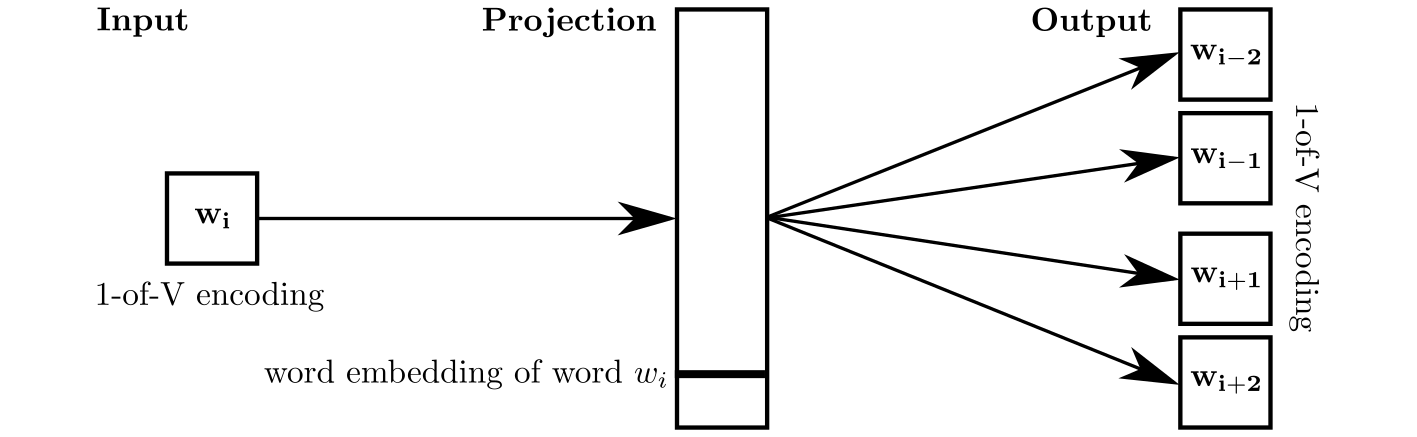
\includegraphics[width=12cm]{figures/skip_gram_architecture.pdf}
       \caption{Skip-gram architecture of word2vec.
       One row in the projection matrix corresponds to the word embedding of one word.
       The marked row at the bottom of the matrix represents the word vector of the current word $w_i$.}
       \label{fig:skip_gram_architecture}
\end{figure}

Mikolov et al.\ presented two models.
The continuous bag-of-words model works by predicting the center word in a symmetric context window.
The continuous skip-gram model works the other way round: given a word, it tries to predict the context.
We focus on the skip-gram model in the following, as it had the better evaluation results in the original paper.
We illustrate its architecture in Figure~\ref{fig:skip_gram_architecture}.
For each training sample, an input word $w_i$ is required to predict its surrounding words $w_{i - C}$, $w_{i - C + 1}$, ..., $w_{i - 1}$, $w_{i + 1}$, ..., $w_{i + C - 1}$, $w_{i + C}$, where $C$ is the context window size.
$C$ is typically between 5 and 15.
The context ends at the end of the sentence so that no cross-sentence training examples are created.
Both the center word as well as the context words are encoded via 1-of-V encoding.
The projection matrix in-between is trained via stochastic gradient descent to predict the context as accurately as possible.
Because of the 1-of-V encoding one training sample activates exactly one row in the projection matrix during the vector-matrix multiplication.
This row is used as the word vector representation of the corresponding word.
% There is exactly one projection matrix $M$ in between, which is trained to predict the context as accurately as possible.
% The matrix is trained via stochastic gradient descent with the following objective:
% \begin{align*}
%   \frac{1}{T} \sum\limits_{t=1}^{T} \sum\limits_{-C \leq i \leq C, i \neq 0} \log~&p(w_{t + i} | w_t),~where\\
%   &p(w_c | w_i) = \frac{\exp (v_{i} * M)}{\sum_{v=1}^{|V|} \exp (v_{v} * M)},
% \end{align*}
% where $T$ is the number of training samples in the current sentence.
% The idea is to maximize the probability of the training samples by adjusting the weights in $M$.
% Due to the 1-of-V encoding, each input word activates exactly only one row in the projection matrix.
% This row is the word embedding for the input word.
In the skip-gram model, surrounding words have to be encoded in the word vector for each word or as Mikolov et al.~\cite{Mikolov2013} state ``vectors can be seen as representing the distribution of the context in which a word appears''.

A nice property of the trained word vectors is, that linear relationships between words are kept in the vector space.
It was shown that
\begin{equation}
  \vec{v}_{king} - \vec{v}_{man} + \vec{v}_{woman}
\end{equation}
is closest to the vector representation of the word ``queen''~\cite{Mikolov2013b}.
Interestingly, this relationship holds for both semantic and syntactic similarly~\cite{Mikolov2013a}, such as
\begin{equation}
  \vec{v}_{houses} - \vec{v}_{house} + \vec{v}_{car}
\end{equation}
is closest to $\vec{v}_{cars}$.
% Quote from webpage: This seems to be a great strength of neural networks: they learn better ways to represent data, automatically. Representing data well, in turn, seems to be essential to success at many machine learning problems. Word embeddings are just a particularly striking example of learning a representation.

Word embeddings have been used in many natural language and machine learning tasks.
They are a natural input to many machine learning algorithms, as they provide a better encoding than the traditional one-hot encoding.
Concrete use cases involve statistical language modeling, machine translation~\cite{Zou2013}, sentiment analysis~\cite{Maas2011} and paraphrase detection~\cite{Mikolov2013a}.

% A word vector can be seen as a summary of the word with all its meanings.
% Many applications require not only word vectors, but also summaries of longer chunks of text.
% Therefore, it is necessary to embed sentences or documents in the word embedding space.
% For this problem, Le and Mikolov~\cite{Le2014} proposed paragraph vectors.
% In their work, paragraph can mean an arbitrary long text, ranging from sentences to entire documents.
% Paragraph vectors are trained by adding an artificial word to each context, which represents the current paragraph.
% These paragraph vectors can then be viewed as a summary of the meaning of the entire paragraph, which is useful for further downstream applications.
%for sentiment analysis by training logistic regression classifier on the vectors.
% http://sentic.net/sentire2011ott.pdf

% \subsubsection*{Implementations}
% The original implementation of the approach by Mikolov et al.~was open sourced under the name word2vec.
% It is implemented in C and can be used as a command line tool.
% There also exists another implementation in the gensim package by {\v R}eh{\r u}{\v r}ek~\cite{Rehurek2010}.
% These two implementations can run multi-threaded in the CPU.
% There also exist some GPU implementations, however, these are not as stable.
% Therefore, we will concentrate on the CPU implementations first.

\section{Comparison between LDA and word embeddings}

After we presented topic models and word embeddings separately in the last sections, we will now compare the models and analyze their strengths and weaknesses.
At their foundations, LDA and word embeddings come from different backgrounds.
LDA stems from Bayesian statistics, while word embeddings were first developed in the neural-network and deep learning community.
Both methods use the distributional hypothesis~\cite{Firth1957}, that says, that similar words tend to occur together.
% Baroni et al.~\cite{Baroni2014} show, that both methods fundamentally are based on the assumption that ``semantically similar words tend to have similar contextual distributions''.
However, the methods use this hypothesis to come to different conclusions.
LDA works on the bag-of-words assumption, i.e.\ it treats a document as a whole and does not use the order of the words.
When making a prediction for the next word, LDA makes a global prediction based on the topic distribution in the current document.
Word embeddings, on the other hand, generate the next word based only on a small context of the word and are per se local.
%%%% Edited out by Ralf, because of repetition. Probably try to incorporate the important parts from here (local-global, distributional hypothesis) in the earlier chapters.

Both LDA and word embeddings can provide a vector representations for words.
In LDA, this works by taking the topic distribution for a word as the embedding in the topic space.
However, this representation is not good at keeping linear relationships~\cite{Mikolov2013b,Mikolov2013a}.
Also, it tends to yield sparse vectors as LDA tries to keep the number of topics per word small.

The different nature of the models is also represented in the standard evaluation method for each.
Topic models are typically evaluated using topic coherence, i.e. how well the top words from the topics belong together and have a common, easily identifiable theme.
Word embeddings, on the contrary, are typically evaluated using word similarity tasks or word analogy reasoning tasks.
When building new topic models, which use word embeddings, our goal is to incorporate a priori semantic information about words into the topic model.
The assumption is, that words which are close to each other in the embedding space should have a higher probability to occur in the same topic together.

Baroni et al.~\cite{Baroni2014} introduce the classification of count-based methods and prediction-based methods in distributional semantic models.
Prediction-based methods try to set word vectors so that they are able to predict the context words.
Count-based methods are based on counting the occurrence of words and co-occurrence with other words.
Popular count-based methods typically use pointwise mutual information (PMI) and matrix transformation on the co-occurrence matrix.
While word embeddings are clearly a prediction-based method, LDA constitutes a hybrid type in this classification.
LDA is based on word counts and co-occurrences and treats words as discrete observations, however, the model parameters are chosen to maximize its predictive power.

Another aspect is the interpretability of the model.
LDA forces the elements in a vector to sum up to one and all values must be non-negative.
Thus, the embedding of a word in the topic space is easily interpretable by humans.
With a word vector of $[0~0~0.2~0.8]$ and given the meanings of a topic, a word can be interpreted, for example, as being used $20~\%$ in \emph{sports} and $80~\%$ in \emph{politics}.
When working with word embeddings, a vector like $[{\text{-}2.4}~0.3~1.3~{\text{-}0.1}]$ is not interpretable.
The arbitrary dimensions and values of a word embedding vector cannot be understood by humans.

Regarding the performance, LDA operates much slower than word embeddings, when the training set size is equal.
LDA becomes expensive on large data sets, partially because the inference problem is NP-hard~\cite{Sontag2011a}.
For training, the entire corpus and the topic assignments have to fit in main memory.
Also, when the number of documents is increased, the number of topics to represent the corpus usually needs to be increased as well, which further slows down the inference.
The method by Mikolov et al.\ has been successfully trained on a corpus with about 100 billion words, thus showing that it scales to large data sets.

\section{Existing combinations}
The recent popularity of word embeddings has led to a re-evaluation of topic models.
There are two directions for research in this area.
% The existing related work, which combines topic modeling approaches with word embeddings, can be roughly divided in two directions.
One type of model tries to improve topic models by incorporating word vectors into the model.
As LDA is based on the bag-of-words model, no relationship between words is encoded in the model.
The prior knowledge about semantically similar words, that word embedding models provide, is used to create more coherent topic models.
The other type of model aims to improve word embeddings by incorparating ideas from topic models.

% In this section, we will present existing topic models, which use word embeddings, in detail.
% Afterwards, we give a short overview over improved word embeddings.
% We will present existing models in this area in the rest of section in detail.
% We summarize the prior work in this field in Table~\ref{table:tm_and_we_combinations}.\footnote{ToCoh: Topic Coherence; WordSim: Word Similarity; DocClass: Document Classification; DocClust: Document Clustering; Analogy: Word Analogy Reasoning; SentComp: Sentence Completion}

% \begin{sidewaystable*}
%        \centering
%        \caption{Overview over related work of combinations between topic models (TM) and word embeddings (WE) and how they have been evaluated}
%        \begin{tabular}{lcccccccc}
%          \toprule
%               \textbf{Paper}                  & \textbf{TM} & \textbf{WE} & \textbf{ToCoh} & \textbf{WordSim} & \textbf{DocClass} & \textbf{DocClust} & \textbf{Analogy} & \textbf{SentComp} \\
%               \midrule
%               Blei et al.~\cite{Blei2003}     & \cmark &  &                &                  & \specialcell{\cmark\\\textsc{Reuters}}  &                   &  & \\
%               Mikolov et al.~\cite{Mikolov2013a} &     & \cmark &                &           &                      &                   & \cmark & \specialcell{\cmark\\\textsc{Microsoft}\\\textsc{sentence}\\\textsc{completion}} \\
%               Das et al.~\cite{Das2015}       & \cmark &  & \specialcell{\cmark\\Wikipedia\\co-occurrence} &      &                   &                   & & \\
%               Nguyen et al.~\cite{Nguyen2015} & \cmark &  & \specialcell{\cmark\\Wikipedia\\co-occurrence} &      & \specialcell{\cmark\\\textsc{20-News-}\\\textsc{Group},\\\textsc{TagMyNews}} & \specialcell[h]{\cmark\\Same as\\left} & & \\
%               Sridhar~\cite{Sridhar2015}      & \cmark &  & \specialcell{\cmark\\Manual\\annotation}               &                  &                   &  & & \\
%               % Moody~\cite{Moody2016}          & \cmark & \cmark & \specialcell{\cmark\\Palmetto\footnotemark\\evaluation tool}         & \specialcell{\cmark\\Only\\qualitative} &                      &         & & \\
%               Liu et al.~\cite{Liu2015} &     & \cmark &                & \specialcell{\cmark\\\textsc{SCWS}}    & \specialcell{\cmark\\\textsc{20-News-}\\\textsc{Group}}               &                   &  & \\
%               Cheng et al.~\cite{Cheng2015} &     & \cmark &                & \specialcell{\cmark\\\textsc{SCWS} +\\paraphrase\\detection\\\textsc{MSRPC}}    &  &                   &  & \\
%               % • Nguyen et al.~\cite{Nguyen2015}} & • \parbox[t]{7cm}{Conceptual Text Understand in Distributional Semantic Space, Cheng et al.~\cite{Cheng2015}} \\
%               % • \parbox[t]{7cm}{Unsupervised Topic Modelling for Short Texts Using Distributed Representations of Words, Sridhar~\cite{Sridhar2015}} & • lda2vec, Moody~\cite{Moody2016} \\
% % • Topical Word Embeddings, Liu et al.~\cite{Liu2015}
%               \bottomrule
%        \end{tabular}
%        \label{table:tm_and_we_combinations}
% \end{sidewaystable*}
% \footnotetext{The online evaluation tool can be accessed at \url{http://palmetto.aksw.org/palmetto-webapp}}

\subsection{Improved topic models}

We will now focus on models, which yield improved topic models and present them in the following sections.
\subsubsection{Gaussian LDA}
Das et al.~\cite{Das2015} proposed a method named Gaussian LDA.
In this approach, a topic is no longer a distribution over words in the vocabulary, but a Gaussian distribution in the word embedding space.
Also, words are no longer atomic units, but are represented by their corresponding pre-trained word embeddings.
The authors use word embeddings trained on the English Wikipedia with $M=50$ dimensions, which are not published~\cite{Das2016}.
Each topic $k$ is associated with a mean vector $\mu_k \in \mathbb{R}^{M}$ and a  covariance matrix $\Sigma_k \in \mathbb{R}^{M * M}$.
The prior distribution over the means is a normal distribution and the prior distribution over the covariances is an inverse Wishart distribution $\mathcal{W}^{-1}$, a distribution over symmetric positive-definite matrices.

Three hyperparameters have to be set for Gaussian LDA.
$\nu \in \mathbb{R}$ represents the degrees of freedom for the inverse Wishart distribution and is typically set to the number of dimensions of the word embeddings.
$\Psi$ represents the prior covariance for the inverse Wishart distribution and is set to $3 * \mathbb{I}_M$.
Finally, $\kappa$ represents the strength of the prior for the mean vector.
With these hyperparameters, the generative process of Gaussian LDA can be summarized as follows:
\begin{enumerate}
       \item Fix number of topics $K$ in the document collection
       \item Choose covariance matrix $\Sigma_k \sim \mathcal{W}^{-1}(\Psi, \nu)$ for each topic $k \in \{1~..~K\}$
       \item Choose mean $\mu_k \sim Normal(\mu, \frac{1}{\kappa} \Sigma_k)$ for each topic $k \in \{1~..~K\}$
       \item Now, for each document $d$:
       \begin{enumerate}
              \item Choose topic distribution $\theta_d \sim Dirichlet(\alpha)$
              \item For each position $i$ in the document
              \begin{enumerate}
                     \item Choose topic $z_{d,i} \sim Multinomial(\theta_d)$
                     \item Choose word $w \sim Normal(\mu_{z_{d,i}}, \Sigma_{z_{d,i}})$
              \end{enumerate}
       \end{enumerate}
\end{enumerate}

These parameters are inferred using Gibbs sampling as in standard LDA with the topic sampling equation: % together with linear algebra tricks
\begin{equation*}
  p(z_{d,i} = k | z_{-(d,i)}, V_d) \propto (n_{k,d} + \alpha_k) * t_{\nu_k - M + 1}\Big(v_{d,i} \Big| \mu_k, \frac{\kappa_k + 1}{\kappa_k} \Sigma_k\Big)
\end{equation*}
where $z_{-(d,i)}$ are all topic assignments in all documents except the current word, $V_d$ is the sequence of vectors of the current document, $D$ is the number of dimensions of the word vectors.
The evaluation of the multivariate $t$ distribution requires the determinant and the inverse of the covariance matrices $\Sigma_k$, which is an $\mathcal{O}(M^3)$ operation.
These parameters need to be updated after each word.
The authors provide some performance improvements using linear algebra identities, which improve the runtime to $\mathcal{O}(M^2 * \overline{K_d})$, where $\overline{K_d}$ is the average number of topics in a document.
Usually, $\overline{K_d}$ is much smaller than $K$.
Still, inference in Gaussian LDA is very slow.
We will compare the runtime with other models in Section~\ref{sec:runtime}.

\subsubsection{Latent Feature Topic Models (LFTM)}
Another approach, called Latent Feature Topic Models, is proposed by Nguyen et al.~\cite{Nguyen2015}.
They use word embeddings to sample words not only from the multinomial topic distribution, but also from the embedding space.
Instead of directly sampling a word from the topic-word distribution of the chosen topic, they introduce a Bernoulli parameter $s \sim Ber(\lambda)$.
This parameter decides, whether the word is sampled as usual from the topic-word distribution or from the latent feature vectors.
When sampling in the embedding space, the authors need to define a distribution over all the words.
This is achieved by introducing one topic vector $\tau_t$ for all topics.
This topic vector lies in the same space as the word embeddings.
Then, to sample in the embedding space, the model samples from the following softmax-normalized multinomial word distribution:
\begin{equation*}
    Multinomial(w | \tau_t, \omega) = \frac{exp(\tau_t * \omega_w)}{\sum_{w' \in W} exp(\tau_t * \omega_{w'})},
\end{equation*}
where $\tau_t$ is the representation of topic $t$ in the word embedding space and $\omega$ are the pre-trained and fixed word embedding vectors.
The topic embeddings $\tau_t$ are updated after each iteration of Gibbs sampling via a maximum likelihood estimation based on all other parameters given.
Here, the topic assignments are fixed.
The negative log likelihood including $L_2$ regularization for each topic vector $\tau_t$ is given as:
\begin{equation*}
  L_t(\tau_t) = - \sum_{w \in W} K^{t,w} \Big(\tau_t * \omega_w - \log \sum_{w' \in W} \exp (\tau_t * \omega_{w'}) \Big) + \mu * || \tau_t ||^2,
\end{equation*}
and is minimized with respect to the topic vectors.
$K^{t,w}$ represents the number of times word $w$ occurred with topic $t$.
Optimization is done via L-BFGS~\cite{Liu1989}.

Using the topic vectors, the generative process can be summarized as follows:
\begin{enumerate}
    \item Fix number of topics $K$ in the document collection
    \item Choose word distributions $\phi_k \sim Dirichlet(\beta)$ for each topic $k \in \{1~..~K\}$
    \item Now, for each document $d$:
    \begin{enumerate}
        \item Choose topic distribution $\theta_d \sim Dirichlet(\alpha)$
        \item For each position $i$ in the document
        \begin{enumerate}
            \item Choose topic $z_{d,i} \sim Multinomial(\theta_d)$
            \item Choose binary variable $s_{d_i}$, which decides whether the word is sampled from the multinomial as usual or from the word embedding space
            \item Choose word $w \sim (1 - s_{d_i}) * Multinomial(\phi_{z_{d,i}}) + s_{d_i} * Multinomial(\tau_{z_{d_{i}}} \omega^T)$
        \end{enumerate}
    \end{enumerate}
\end{enumerate}
The authors use pre-trained vectors from word2vec~\cite{Mikolov2013a} and GloVe~\cite{Pennington2014} and conclude that none of these works better than the other.
The optimization of the topic vector and the coupling between the two components make the inference difficult.
As Li et al.~\cite{Li2016} state, ``the implementation is slow and infeasible when applied to a large corpus''.

\subsubsection{Nonparametric Spherical Topic Model (NSTM)}
Batmanghelich et al.~\cite{Batmanghelich2016} introduce nonparametric spherical topic modeling.
They build on top of Gaussian LDA, but argue that Gaussian distributions do not capture the distribution of words in the embedding space well.
Instead they propose the von Mises-Fisher distribution to model topics in the embedding space.
The von Mises-Fisher distribution is a distribution on the hypersphere with a mean direction $\mu$ and a concentration parameter $\kappa$.
The distribution is rotationally symmetric around $\mu$.
If there are only two dimensions, the distribution reduces to the von Mises distribution on the circle.
Using the von-Mises Fisher distribution requires all word vectors to be normalized so they lie on the $M$-dimensional unit hypersphere.

Intuitively, the von-Mises Fisher distribution is a good distribution choice, because its distance function is based on the cosine similarity.
In the Gaussian distributions used by Gaussian LDA, words are picked based on the proximity in the embedding space.
The proximity is measured using Euclidean distance respectively Mahalanobis distance, if the covariance matrix is not the identity matrix.
However, semantic relatedness between words is usually not measured by euclidean distance in embedding models, but rather by cosine distance~\cite{Mikolov2013a}.
The length of the word vectors does not matter for the similarity.
This is exactly what is captured by the von Mises-Fisher distribution.

% The Gaussian LDA model tries to group words in a topic, which are near each other in the embedding space.
% , where proximity is measured by the euclidean distance (or Mahalanobis distance, if the covariance matrix is not 
% In Gaussian distributions the similarity between samples is estimated by Euclidean distance.
% However, in the word2vec approach proposed by Mikolov~\cite{Mikolov2013}, semantic relatedness between words is calculated using cosine similarity.

In the spherical topic model, each topic is represented by a von Mises-Fisher distribution with parameters $\mu_k$ and $\kappa_k$.
A log-normal prior is placed on $\kappa_k$ and a von Mises-Fisher prior is placed on the $\mu_k$'s.
In contrast to the previous models, this model is not based on LDA but rather on hierarchical Dirichlet processes.
These models allow the number of topics to be determined automatically.
% To allow a variable number of topics the document-topic distribution is sampled.
All together, the generative process looks as follows:
\begin{enumerate}
    \item Choose base distribution $\beta \sim GEM(\gamma)$ from stick-breaking distribution
    \item Choose topic direction on unit sphere $\mu_k \sim vMF(\mu_0, C_0)$ for each topic $k \in \{1~..~K\}$
    \item Choose topic concentration $\kappa_k \sim log\mbox{-}normal(m, \sigma^2)$ for each topic $k \in \{1~..~K\}$
    \item Now, for each document $d$:
    \begin{enumerate}
        \item Choose topic distribution $\theta_d \sim DP(\alpha, \beta)$
        \item For each position $i$ in the document
        \begin{enumerate}
            \item Choose topic $z_{d,i} \sim Multinomial(\theta_d)$
            \item Choose word $w \sim vMF(\mu_{z_{d,i}}, \kappa_{z_{d,i}})$
        \end{enumerate}
    \end{enumerate}
\end{enumerate}

The authors propose an effiecient parameter estimation algorithm based on stochastic variational inference.
They use 50-dimensional word embeddings, which they trained on Wikipedia.

\subsubsection{Generative Topic Embedding (TopicVec)}
Li et al.~\cite{Li2016} propose generative topic embeddings and call their system TopicVec.
The main idea compared to LDA is to take the immediate context of a word into account and not only the bag-of-words information.
While LDA picks a word from one of the $K$ multinomial topic distributions, TopicVec defines this distribution based on the context words, similar to the word2vec skip-gram architecture.
For that, they encode a topic with a vector $t_k$ in the embedding space.
This vector is called the ``topic embedding'' of topic $k$.
With these topic embeddings and given the preceding context words, the document and the topic, TopicVec defines the multinomial distribution for a word as follows:
\begin{equation}
  \label{eq:topicvec}
  P(w_c | w_0 : w_{c - 1}, z_c, d_i) \propto \exp \bigg( v_{w_{c}}^T * \Big( \sum\limits_{l=0}^{c-1} v_{w_l} + t_{z_c} \Big) + \sum\limits_{l=0}^{c - 1} a_{w_{l} w_c}  + r_{z_c} \bigg),
\end{equation}
where $c$ is the context window size, $w_c$ is the word at the last position of the current context window, $v_{w_c}$ is the word's vector embedding, $t_{z_c}$ is the topic embedding vector of the topic $z_c$ and $r_{z_c}$ is a normalizing constant.
The terms $a_{w_l w_c}$ are bigram residuals, which capture the relationship between each context word and the target word explictly.
The authors claim, that this method ``exploits the word collocation patterns both at the level of the local context and the global document''~\cite{Li2016}.
The generative process looks as follows:
\begin{enumerate}
    \item Fix number of topics $K$ in the document collection
    \item Choose topic vector $t_k \sim Unif(S_{\gamma})$ from hypersphere of radius $\gamma$ for each topic $k \in \{1~..~K\}$
    \item Now, for each document $d$:
    \begin{enumerate}
        \item Choose topic distribution $\theta_d \sim Dirichlet(\alpha)$
        \item For each position $i$ in the document
        \begin{enumerate}
            \item Choose topic $z_{d,i} \sim Multinomial(\theta_d)$
            \item Choose word $w$ according to the word distribution defined in Equation~\ref{eq:topicvec}
        \end{enumerate}
    \end{enumerate}
\end{enumerate}

The authors provide a variational inference algorithm for TopicVec, which learns the topic assignments and the topic embeddings simultaneously.
As the words are sampled from their context words, the architecture allows to learn topics for a single document.
No word collocation information over different documents is necessary.
However, as no other method offers this possibility, we will evaluate TopicVec with one set of topics for all documents.
In their paper, the authors evaluated the model only on a document classification task.
We will also evaluate topic coherence.

% \subsubsection{Gaussian Mixture Model in Embedding Space}
% Another idea is proposed by Sridhar~\cite{Sridhar2015}.
% They start by training word embeddings.
% Afterwards they fit a Gaussian mixture model directly on the word embedding space.
% A topic is represented by mean and covariance matrix.
% In contrast to Das et al.~\cite{Das2015}, Sridhar~\cite{Sridhar2015} assumes the topics to be fixed given the word embeddings, while Das et al.~\cite{Das2015} only take the embeddings as a basis and still learn the topics based on the word co-occurrences in the corpus.


\subsection{Improved word embeddings}
We will now give a short overview about word embedding models improved by topic models.
Liu et al.~\cite{Liu2015} propose topical word embeddings.
These embeddings make use of word topics inferred via LDA to generate better word vectors.
They propose three different architectures.
The first method regards topic as pseudo words, which are added to the context of each word.
Thus, an embedding for a word and its topic is learned independently.
The second method considers each pair of word and topic as a pseudo word.
The third method works the same way, except that it learns only one word embedding vector per word and one topic embedding vector per topic.
These two vectors are then combined for the vector of the word-topic pair.
The first method performed best in their word similarity and text classification benchmarks.
Using the additional topic information when training word embeddings has practical benefits for similarity evaluation.
When the model is asked for similar words to the word ``apple'', it returns ``peach'', ``juice'', ``strawberry'' or it returns ``mac'', ``ipod'', ``android'' depending on the topic of the word.

A similar idea is used by Cheng et al.~\cite{Cheng2015}.
In fact, the first model they propose is the same as the first model from Liu et al.~\cite{Liu2015}.
Additionally, the propose two models, which do not model the topic and the word independently.
Rather, they divide the task of choosing a word in two steps: ``locating the right concept and then searching for a word underneath the chosen concept''~\cite{Cheng2015}.
These models, called generative word-concept skip-gram, outperform the skip-gram architecture on paraphrase identification and Q-A relatedness classification.

Moody~\cite{Moody2016} proposes lda2vec.
His method learns word vectors together with learning topic vectors and an intuitive topic-based document interpretation.
Even though trained in the word embedding space, the topic-document vectors are still kept sparse to be interpretable for humans.
However, the method is not evaluated extensively and it is unclear, whether this method yields improved word vectors.

% FROM MIKOLOV COLING 2014 tutorial
% Sentence-level representations
% • To obtain sentence level representations, we can add unique tokens
% to the data, one for each sentence (or short document)
% • These tokens are trained in a similar way like other words in the skipgram
% or CBOW models, just using unlimited context window (within
% the sentence boundaries)


%one is supervised, the other one is unsupervised

%``A long tradition in computational linguistics has shown that contextual information provides a good approximation to word meaning, since semanti- cally similar words tend to have similar contex- tual distributions (Miller and Charles, 1991).''
%``It remains to be seen whether the two types of models are complementary in the errors they make, in which case combined models could be an interesting av- enue for further work.''
%there has been a shift from the LDA to the word embeddings


% \begin{itemize}
       % \item
       %        Directly run a GMM on the word embedding space --> See Gaussian LDA
       % \item
       %        Run LDA first.
       %        Then run word embedding training, except that the word also has to predict the surrounding context.
       %        Problem: LDA performance
       % \item
       %        Run LDA first.
       %        Then run word embedding training, except that the same word from different topics gets a unique token
       %        Problem: LDA performance
       % \item
       %        Try to interpret word embedding dimensions using topic models.
       %        This requires a labelled topic model, i.e.\ topic 40 is about sports.
       %        Then try to put a label on a word embedding dimension, for example, the large the value in dimension x the more about sports.
       % \item
       %        Run LDA, then calculate average word vector and covariance matrix for all topics.
       %        Check, how well the topics are distributed in the topic space.
       %        This also allows to assign unseen words to a topic.
% \end{itemize}

% \section{Preprocessing}
% No-stemming (does harm in both word2vec and topic modeling), as it destroys the difference between Apple and apples and (other example) as well as small/smallest.
% Quoting lots of stuff from the lda2vec

% \section{Enhancing topic models?}
% Then we need evaluation for topic models and show that they are better
% Use pre-trained word vectors to improve~\cite{Das2015}

% \section{Bayesian optimization}
% \begin{itemize}
%   \item Good for noisy black-box functions, when evaluations are costly, no derivative and the problem is non convex
%   \item Builds a statistical model for the function from the hyperparameter space to the evaluation function
%   \item By using the information of all previous runs, the framework can suggest a new point to which provides max information
%   \item balances \emph{exploration} (checking previously unknown points in the hyperparameter space) vs. \emph{exploitation} (using the current best values to check nearby points in the hyperparameter space)
%   \item $\Rightarrow$ fewer experiments are necessary
%   \item \url{https://github.com/HIPS/Spearmint}
% \end{itemize}


\chapter{WELDA -- Word embeddings in LDA}
\label{sec:welda}

In this chapter, we start with a series of experiments with word similarity calculations in topic models and embedding models, that motivate our newly-developed approach.
We will then present our approach, which is based on re-sampling words using information from the word embedding models.
Our model, called WELDA (for \textbf{W}ord \textbf{E}mbedding \textbf{LDA}), is a new type of topic model which leverages information from word embeddings.
We will present the modified Gibbs sampling algorithm and then discuss a series of important design decisions.
Afterwards we will analyze the different topic models and word embedding-enhanced topic models in two standard tasks for topic models: topic coherence and document classification.

\section{Approach}
In this section, we describe the main ideas behind WELDA.
We show and explain the algorithm and discuss different design decisions and parameters.

\subsection{Motivation}
We aim to combine the two methods to achieve better topic models.
As word embeddings and LDA topic modeling are techniques from different backgrounds and with no inherent relationship to each other, we started with exploring how the results of one can be interpreted in the other model.
To this end, we ran initial experiments on the Wikipedia corpus\footnote{Full English Wikipedia dump from June 21st, 2016}, on which we trained both a topic model and a skip-gram word embedding model with two hundred dimensions.
We then evaluated the similarities between the words to understand the different strengths of both models.
For embedding models, we used the cosine similarity between the two vectors.
For topic models, we built the topic distribution of a word by retrieving the word's probability in all topics in the topic-word matrix.
We then normalized these probabilities to one and treat it as a distribution.
To calculate the similarity between two words, we calculated the Jensen--Shannon divergence, which is a symmetrized and smoothed version of the Kullback--Leibler divergence~\cite{Kullback1951}:
\begin{equation*}
  JSD(P~||~Q) = \frac{1}{2} KL(P~||~M) + \frac{1}{2} KL(Q~||~M),~where~M = \frac{1}{2} ( P + Q)
\end{equation*}
When using base two logarithm for the Kullback--Leibler divergence, the Jensen--Shannon divergence is between zero and one, where zero corresponds to the highest similarity, because the probability distributions are identical.
We therefore use $1 - JSD(P~||~Q)$ as the similarity metric.

Even though both word embeddings and topic models exploit the distributional hypothesis~\cite{Firth1957} the correlation of word similarities is surprisingly low.
We calculated the similarities of all word pairs created from the top ten words of an LDA topic model trained on Wikipedia.
The similarities of word embeddings and the topic model only correlate with $R_{Pearson} = 0.30$.
The results were similar, when we used Hellinger distance or Bhattacharyya distance as the similarity measure for probability distributions in the topic model.

When looking at example pairs of high/low similarity in both models in Table~\ref{table:tm_and_we_word_similarities}, we see that topic models are able to detect more far-fetched, less obvious connections.
This is a good property of topic models, however it sometimes makes the main theme hard to understand.
% This is a goot thing! Better examples?
Embedding models, on the other hand, assign high similarity to immediately obvious word pairs, often direct replacements of each other.

\begin{table*}
       \ra{1.2}
       \centering
       \caption{Typical examples for different notion of word similarity in topic models and word embeddings.
       For example, the word pair \emph{war, commander} in the cell \emph{high topic model similarity, low word embedding similarity} means, that this pair is assigned a low similarity in the embedding space, but high similarity in the topic model space.
       High similarity indicates a similarity value in the upper quartile, low similarity corresponds to a value in the lower quartile.}
       \begin{tabular}{p{2cm}cp{2cm}p{4cm}p{4cm}}
       \toprule
         \textbf{}                                                                                  &  & \textbf{} & \multicolumn{2}{c}{Word embedding similarity} \\
                                                                                                  &&           & High                      & Low                       \\ \midrule
         \multirow{2}{*}{\begin{tabular}[c]{@{}c@{}}\\ Topic model\\ similarity\end{tabular}} && \vspace{0.1cm}High    &
           disease, diseases \newline
           professor, lecturer \newline
           poetry, prose
           &
           africa, uganda \newline
           war, commander \newline
           rights, discriminated \\
           && \vspace{0.05cm}Low       &
           catalan, galician \newline
           prestige, respectability \newline
           obscenity, sedition
           & \emph{completely unrelated \newline words} \\
           \bottomrule
       \end{tabular}
       \label{table:tm_and_we_word_similarities}
\end{table*}

We also evaluated both model types on a standard similarity benchmark.
We used the \textsc{WordSim-353}~\cite{Agirre2009} data set.
This data set contains 353 word pairs, whose similarity was assessed by thirteen to sixteen human annotators each.
The subjects were asked to rate the pair from zero (totally unrelated words) to ten (very much related or identical words).
The highest-rated pair was \emph{midday -- noon} (9.29) and the lowest-rated pair was \emph{king -- cabbage} (0.23).
We calculated the correlation between the human ratings and the model's ratings for both the embedding and topic model using the above mentioned similarity metrics.
Embedding model excel at this task, matching the human ratings with $r_{Pearson} = 0.66$, while the topic model only achieves $r_{Pearson} = 0.49$.

To summarize, syntactic variations and more direct connectedness play a bigger role in word embedding models, while topic models often capture more loose relationships.
Embedding models are good at assessing similarity between words.
These observations make us believe that word embeddings can help create more coherent topic models.
% We take this as motivation to create topic models, whose topics 
Our goal is to strengthen the topic themes by augmenting the top topic words with similar words from the word embedding space, but at the same time not disregarding the bag-of-words collocation information in the documents completely.
This way, we help the user understand the common theme in a topic better, while still creating an overview over the entire corpus by looking at all topics.

\subsection{WELDA Algorithm}

We base our new topic modeling technique on the observations from the last chapter.
Word embedding models are trained on predicting a certain word at an exact position.
That means, if we look at the similar words for a given word, the model predicts a word which could have been at the same position.
The goal is to transfer probability mass in the topic model more towards these words, which could have occurred at the same position.

We achieve this by sampling new words from the embedding space.
For this, we learn a multivariate continuous distribution in the embedding space for each topic.
The choice of distribution can be varied and will be explained later.
We call each of this distributions a \emph{topic distribution}.
This topic distribution is estimated from the top words of each topic and their representation in the embedding space.
% By sampling new words from this distribution during the Gibbs sampling, we make
We then selectively replace words in the text with words from the topic distribution.
We achieve this by sampling a new word in the innermost loop of the Gibbs sampling algorithm and then proceeding as if that newly sampled word appeared.
These words have a high similarity to the top words in the topic.

We now describe the algorithm in more detail.
We first start with an initialization step, which is shown in Algorithm~\ref{alg:welda_init}.
Before running the Gibbs sampling, we load a word embedding model (line 2).
For all words in the corpus, we then retrieve its high-dimensional representation in the embedding space (line 3-4).
Afterwards, we use principal component analysis (PCA) to project the word vectors to a lower number of dimensions (line 5).
Finally, using the lower-dimensional new word vectors, we initialize a datastructure, that allows us to quickly find the nearest word given a vector in the embedding space (line 6).
We use either locality-sensitive hashing (LSH) or k-d trees depending on the number of dimensions.
We will explain this implementation detail later.

% bad topic words
% For example, imagine
% Two highly similar brands
% however, never occuring together
% but in very similar contexts

\begin{algorithm}
  \caption{Initialization for the WELDA model, to be run before the Gibbs sampling}
  \label{alg:welda_init}
  \begin{algorithmic}[1]
    \Procedure{Init}{array of strings $words$}
    \State{$v \gets load~word~embeddings~from~disk$}
    \For{i $\in$ \{ 1 .. $|words|$ \}}
      \State{$embedding\_matrix[i] = v.get\_word(words[i])$}
    \EndFor
    \State{$embedding\_matrix \gets PCA(embedding\_matrix, N_{pca})$}
    \State{$nn\_search \gets \textit{initialize LSH structure or k-d tree for nearest neighbour search}$}
    \EndProcedure
  \end{algorithmic}
\end{algorithm}

We then proceed with a modified version of the Gibbs sampling algorithm, which is displayed in Algorithm~\ref{alg:welda_gibbs_sampling}.
For the original Gibbs sampling implementation, see Section~\ref{sec:lda}.
As an important first step, we run the standard LDA algorithm until convergence.
Only then we will run some additional Gibbs sampling iterations using our modified Gibbs sampling.
We run LDA first to obtain stable topic assignments and to start with relatively good topics as a baseline.
This is important, because before each Gibbs sampling iteration we estimate the topic distributions for all topics (line 4).
We use this topic distributions later in the innermost loop of the sampling algorithm.
If a coin flip with success probability $\lambda$ succeeds (line 12), we sample a vector from the word embedding space (line 13), based on the topic distribution of the new topic of the current word.
We then use the previously initialized LSH or k-d tree data structure to find the nearest word to our drawn sample (line 14).
Afterwards, we update the counts in the document-topic matrix and in the topic-word matrix, as if we had observed the sampled word and not the word we observed in the text (lines 15-16).

\begin{algorithm}
  \caption{Gibbs sampling algorithm for the WELDA model}
  \label{alg:welda_gibbs_sampling}
  \begin{algorithmic}[1]
    \Procedure{GibbsSampling}{Documents D, Topics Z}
    \State $\textit{initialize topic variables } z_{d_i} \textit{ by running standard LDA for } M \textit{ iterations}$
    \For{$n \in \{\textit{ 1 .. N }\}$}
      \State{\textsc{EstimateDistributionParameters()}}
      \For{$d\_idx \in \{\textit{ 1 .. $|D|$ }\}$}
        \State{$doc \gets D[d\_idx]$}
        \For{$w\_idx \in \{\textit{ 1 .. $|doc|$ }\}$}
          \State{$w \gets doc[w\_idx]$}
          \State{$t \gets Z[d\_idx][w\_idx]$}
          \State{\textit{decrement Z counters}}
          \State{$t \gets sample\_new\_topic(Z)$}
          \If{$coin\_flip(\lambda)\textit{ is successful}$}
            \State{$sample \gets sample\_from\_distribution(t)$}
            \State{$\textit{// update $w$, as if we had seen another word}$}
            \State{$w = nn\_search.find\_nearest\_word(sample)$}
          \EndIf
          \State{\textit{increment Z counters}}
        \EndFor
      \EndFor
    \EndFor
    \EndProcedure
  \end{algorithmic}
\end{algorithm}

As a remaining step, we will explain how we estimate the topic distributions.
This algorithm is detailed in Algorithm~\ref{alg:welda_parameter_estimation}.
For that, we use the top words in all topics and retrieve their respective word vectors (lines 3-4).
We then estimate a multivariate continuous distribution in the embedding space (line 5).

\begin{algorithm}
  \caption{Estimating distribution parameters for each topic, ran before each Gibbs sampling iteration}
  \label{alg:welda_parameter_estimation}
  \begin{algorithmic}[1]
    \Procedure{EstimateDistributionParameters()}{}
    \For{$topic\_id \in \{\textit{ 1 .. $K$ }\}$}
      \State{$top\_words \gets$ \textit{Get top $N_{top}$ words in topic $topic\_id$}}
      \State{$topic\_vectors \gets [embedding\_matrix[word]~for~word~in~top\_words]$}
      \State{$topic\_distributions[topic\_id] \gets estimate\_distribution(top\_vectors)$}
    \EndFor
    \EndProcedure
  \end{algorithmic}
\end{algorithm}

There are several configurable parameters in the algorithm, which we will detail in the following:
\begin{itemize}
  \item \textbf{Choice of topic distribution} (Algorithm~\ref{alg:welda_gibbs_sampling}, line 13 and Algorithm~\ref{alg:welda_parameter_estimation}, line 5):
    We tested three distributions for the topic distributions.
    First, we used the well-known multivariate Gaussian distribution.
    Second, we also tested a Gaussian mixture model.
    Last, by inspiration of Batmanghelich et al. \cite{Batmanghelich2016}, we used the multivariate von Mises-Fisher distribution, a distribution on the hypersphere.
    According to the authors, this distribution is ``well suited for directional data'' and can leverage word similarity correlations better \cite{Batmanghelich2016}.
    We demonstrate these three in detail in the next sections.
  \item \textbf{Resampling probability $\boldsymbol{\lambda}$} (Algorithm~\ref{alg:welda_gibbs_sampling}, line 12):
    The parameter $\lambda$ governs, how often a word is resampled from the topic distributions.
    Running WELDA with $\lambda = 0.0$ corresponds to standard, unmodified LDA and will not have any effect on the model, because we already start with a converged topic model.
    With $\lambda = 1.0$, no single word is taken from the text, rather all words are sampled from the embedding space.
    This parameter governs, how much extra information from the word embeddings is leaked into the topic model.
  \item \textbf{Number of top words for distribution estimation $\boldsymbol{N_{top}}$} (Algorithm~\ref{alg:welda_parameter_estimation}, line 3):
    We are using the top words of each topic to estimate the distributions.
    Usually only the first words of a topic share a common theme.
    % TODO: Number of top words vs. topic coherence.
  \item \textbf{Number of dimensions for dimensionality reduction $\boldsymbol{N_{pca}}$} (Algorithm~\ref{alg:welda_init}, line 5):
    Before estimating the multivariate distribution in the embedding space, we project the high-dimensional embedding space to a lower space.
    There is a tradeoff between the $N_{pca}$ parameter and the $N_{top}$ parameter.
    The lower the final dimension number, the less words we need for estimating the distribution.
    Less words means, that we can only use the really good top words in a topic, and not the later ones.
    On the other hand, by projecting the space to a lower dimension, we throw away semantic information in the embedding space and the similarity between words becomes less reliable.
  \item \textbf{Dimensionality reduction method} (Algorithm~\ref{alg:welda_init}, line 5):
    We use principal component analysis (PCA) to reduce the number of dimensions while maximizing the variance for all remaining dimensions.
  % \item \textbf{Distance function for the nearest neighbour search} (Algorithm~\ref{alg:welda_init}, line 6):
  %   For the nearest neighbour search, ``near'' can be defined by either euclidean distance or cosine similarity.
  %   We expect cosine distance to perform better as it is usually used for evaluating similarity in the embedding space.
  \item \textbf{Number of iterations to run LDA} (Algorithm~\ref{alg:welda_gibbs_sampling}, line 2):
    We usually run $M = 1500$ iterations, as this yields stable topic assignments and is also used in literature~\cite{Nguyen2015}.
    As visible in Figure~\ref{fig:ll_lda_convergence}, the log-likelihood has already converged with that many iterations.
    \begin{figure}
           \centering
           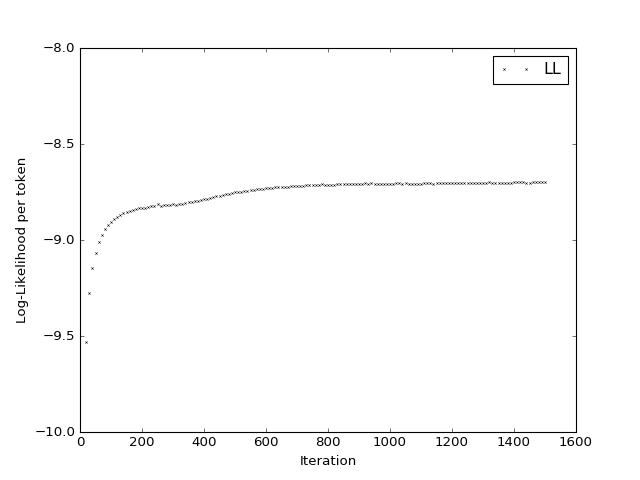
\includegraphics[width=10cm]{figures/ll_lda_convergence.png}
           \caption{Convergence of the LDA model on the \textsc{20News} corpus}
           \label{fig:ll_lda_convergence}
    \end{figure}
  \item \textbf{Standard LDA parameter $\boldsymbol{\alpha}$ and $\boldsymbol{\beta}$}:
    As in standard LDA, the Dirichlet hyperparameters must be chosen.
    We always use the same parameters we use for the initial LDA iterations for the WELDA iterations.
\end{itemize}

\subsection{Different topic distributions}

There are different choices for the topic distributions, which we estimate independently for each topic.
We tested three different multivariate, continuous distributions, which we detail in the following.

\subsubsection{WELDA with Gaussian distributions}

When using a Gaussian distribution, sometimes also called normal distribution, we need to estimate two parameters: the mean vector $\mu \in R^n$ and the covariance matrix $Q \in R^{n * n}$.
The mean can be estimated with the sample mean.
Assuming a Gaussian distribution in the embedding space, an unbiased maximum likelihood estimator of the covariance matrix $Q$ is given as:
\begin{equation*}
  Q = \frac{1}{N_{top}} \sum\limits_{i=1}^{N_{top}} (x_i - \bar{x}) (x_i - \bar{x})^T,
\end{equation*}
where $x_i$ are the vector representations of the top topic words and $\bar{x}$ is the average of these vectors.
\subsubsection{WELDA with von Mises-Fisher distributions}
The von Mises-Fisher distribution has two parameters, the mean direction $\mu$ and the concentration parameter $\kappa$.
The distribution is rotationally symmetric around the mean direction and the higher $\kappa$ the higher the density around the mean.
The lower $\kappa$ the closer the distribution becomes to the uniform distribution on the hypersphere.
As the distribution is only defined on the hypersphere, we have to normalize all word vectors to unit length.
For estimating the mean direction $\mu$ we can again use the sample mean.
For the concentration parameter $\kappa$, there is no maximum likelihood closed form solution, ``because of a difficult transcendental equation that needs to be solved'' \cite{Sra2012}.
We follow Sra~\cite{Sra2012} and use an approximate solution, which is calculated as follows:
\begin{align*}
  \kappa &= \frac{\bar{R}(N_{pca} - \bar{R}^2)}{1 - \bar{R}^2},~where \\
  \bar{R} &= \frac{|| \sum_{i}^{N} x_i ||}{N_{top}} \\
\end{align*}
% The variable $p$ represents the number of dimensions and is equal to $N_{pca}$ in our approach.
This initial approximation can be improved with a few iterations of Newton's method and the following formula:
\begin{align*}
  \kappa_{n + 1} &= \kappa_n - \frac{A_{N_{pca}}(\kappa_n)-\bar{R}}{1-A_{N_{pca}}(\kappa_n)^2-\frac{N_{pca}-1}{\kappa_n}A_{N_{pca}}(\kappa_n)},~where \\
  A_{p}(\kappa) &= \frac {I_{p/2}(\kappa)} {I_{p/2-1}(\kappa)}
\end{align*}
and $I_{v}$ denotes the modified Bessel function of the first kind at order $v$.

\subsubsection{WELDA with Gaussian mixture models}
The Gaussian mixture model fits multiple Gaussian distributions to the embedding space.
Each distribution is characterized by the mean and the covariance matrix.
Additionally, a mixture model provides the mixture weights $\pi_i$, which have to sum to one.
We learn the mixtures by using the expectation-maximization algorithm.
We test different number of mixtures from one up to four and choose the one with the lowest Bayesian information criterion (BIC) by Schwarz~\cite{Schwarz1978}.
Steele et al.~\cite{Steele2009} showed, that the BIC clearly outperforms other methods for choosing the number of mixtures in a Gaussian mixture model.
The BIC is defined as follows:

\begin{equation*}
  BIC = {-2 \cdot \ln{\hat L} + k \cdot \ln(n)},
\end{equation*}
where $\hat{L}$ is likelihood of the model, $k$ is the number of free parameters and $n$ is the number of observations.
$\hat{L}$ can be calculated after learning a model and $n$ is equal to $N_{top}$ in our case.
The number of free parameters $k$ for a Gaussian mixture model is:
\begin{equation*}
  k = (d - 1) + (d * n_{components}) + (n_{components} * d * (d + 1)/2),
\end{equation*}
where $d$ is the number of dimensions and corresponds to $N_{pca}$ in our case.
The first term corresponds to the mixture weights, which have to sum to one.
The second term corresponds to the means of all Gaussian.
The last term calculates the number of free parameters in the symmetric covariance matrix.

\section{Implementation details}

After we presented the main ideas behind WELDA, we now go into detail in some important implementation details.
We discuss the nearest neighbour search, how we fix the vocabulary mismatch between embeddings and topic models, how we deal with often occuring words and why we run LDA initially.

\subsection{Nearest neighbour search}
After we obtained a sample from the topic distribution, we want to find the closest word to our sample in the embedding space (see line in Algorithm~\ref{alg:welda_gibbs_sampling}).
The naive algorithm uses linear search and evaluates all words in the embedding space.
This is very expensive, especially because it happens in the innermost loop of Gibbs sampling and is therefore executed very often, approximately $\lambda * N * N_{words}$ times, where $N_{words}$ represents the number of words in the entire corpus.
However, there are methods with a better runtime: we use two either k-d trees or locality-sensitive hashing depending on the number of dimensions.
K-d trees by Bentley~\cite{Bentley1975} aranges the points in a tree structure, which allows to retrieve the nearest neighbour in $\mathcal{O}(\log n)$ on average.
K-d trees are guaranteed to find the nearest neighbour.
However, for high dimensions, the search degenerates to the linear search due to the curse of dimensionality.
Thus we use locality-sensitive hashing (LSH) by Indyk et al.~\cite{Indyk1998} for higher dimensions.
LSH is an approximate method, i.e. it is not guaranteed that the nearest neighbour is found.
LSH uses a hash-function based on random hyperplanes in the space to bucketize all vectors.
Then, for a new vector, the same hash function is applied and only the bucket with the corresponding hash value must be checked.
LSH has the opposite property, i.e. the lower the number of dimensions the longer it takes.

% https://www.youtube.com/watch?v=Arni-zkqMBA
We therefore evaluated the runtime of the two approaches during a WELDA run.
Figure~\ref{fig:lsh_vs_kdtree} shows the ratio of the runtime of the k-d tree and LSH.
Note the logarithmic y-axis, so the ratio actually increases very fast.
We see, that up to five dimensions including, the k-d tree is faster for looking up the nearest neighbour.
For six or more dimensions, LSH is preferred.
We pick the best method automatically in the $\textsc{Init}$ method in Algorithm~\ref{alg:welda_init}.
\begin{figure}
       \centering
       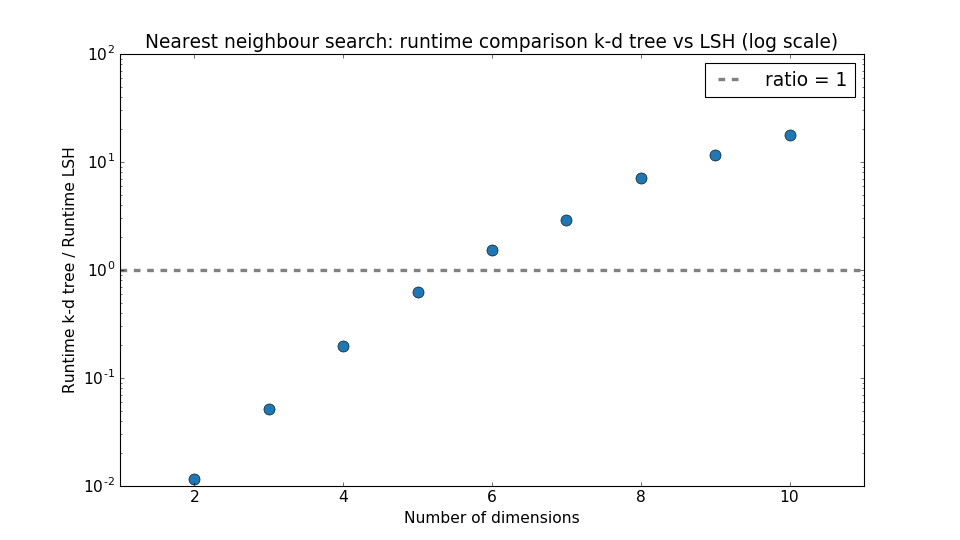
\includegraphics[width=12cm]{figures/lsh_vs_kdtree.png}
       \caption{Performance comparison of LSH and k-d tree for the nearest neighbour word search, based on the number of dimensions.}
       \label{fig:lsh_vs_kdtree}
\end{figure}

\subsection{Vocabulary mismatch between word embeddings and topic model}
\label{sec:vocabulary_mismatch}
The typical preprocessing steps for topic models include lowercasing and stop-word removal~\cite{Boyd-graber2014}.
On the other side, Mikolov~\cite{Mikolov2013d} recommends almost no preprocessing except sentence detection.
Especially stop words are not removed in the word2vec approach by Mikolov:
Due to the window-based approach, where a word predicts its context words at the exact location, this stop word removal would decrease performance.

This different preprocessing leads to different vocabularies and matching those is an important part of preprocessing for WELDA, because we need a word vector for every word.
Otherwise, we can neither calculate the topic distributions nor find the word in the nearest neighbour search.
As the lowercasing step for topic models loses information, the matching is only approximate.
We display the matching process in Algorithm~\ref{alg:vocabulary_matching}.
We try finding the word itself, a capitalized version (first letter is uppercased) and an uppercased version of the word.
We discard all words that we cannot match in this way.

\begin{algorithm}
  \caption{Looking up words in the embedding model}
  \label{alg:vocabulary_matching}
  \begin{algorithmic}[1]
    \Procedure{word2Vec.get\_word}{string $w$}
    \If{w exists in embeddings}
      \State{}
      \Return {array of floats for word w}
    \ElsIf{w.capitalized() exists in embeddings}
      \State{}
      \Return {array of floats for word w.capitalized()}
    \ElsIf{w.uppercased() exists in embeddings}
      \State{}
      \Return {array of floats for word w.uppercased()}
    \Else
      \State{discard $w$}
    \EndIf
    \EndProcedure
  \end{algorithmic}
\end{algorithm}

\subsection{Background topic for corpus-specific stop words}
\label{sec:background_topic}
To speed up the topic improvement process, we detect corpus-specific stop words in addition to the general English-language stop words we use (see Section~\ref{sec:data_sets}).
We detect these stop words automatically during the initial LDA Gibbs sampling.
Instead of using a symmetric Dirichlet $\alpha$ prior for all topics, we multiply the $\alpha_0$ prior by a factor $\alpha_0^{boost}$.
By increasing the value of $\alpha_0$ we force the first topic to appear in almost all documents.
This forces LDA to put words in this topic, which occur in many documents and are very generic.
We call this first topic the \emph{background topic}, because it occurs in many documents as the generic word background for the more informative topics.
We call the corpus-specific stop words background words.

We experimented with different values of $\alpha_0^{boost}$ and show the results in Table~\ref{table:alpha0_boost}.
The second row shows the percentage of documents containing the background topic and the third row shows the percentage of words in the background topic.
We see, that a value of fifteen is sufficient, so that the background topic occurs in more than ninety percent of the documents.
\begin{table}[]
  \ra{1.2}
  \centering
  \caption{Testing by which factor $\alpha_0$ must be multiplied, so that the background topic occurs in many documents.
  All values are percentages.}
  \label{table:alpha0_boost}
  \begin{tabular}{ccccccccccc}
    \toprule
    $\alpha_0^{boost}$                & 1     & 2     & 3     & 5     & 7     & 9     & 10    & 15    & 20    & 30    \\
    \midrule
  doc. containing background topic  & 11  & 23  & 39  & 47  & 56  & 65  & 79  & 90  & 91  & 91  \\
  words in background topic & 2   & 4   & 8   & 10  & 13  & 16  & 19  & 24  & 24  & 24 \\
    \bottomrule
  \end{tabular}
\end{table}
Indeed, if we look at the top words in the background topic in the \textsc{20News} corpus, we find corpus-specific stop words: \\
\noindent\fbox{
    \parbox{0.8\textwidth}{
would one writes like article think get know time people even good much well way make see really want apr right also going still say sure since first something back thing never take many better may things}
}

We treat the thirty top words in the background topic specially.
Whenever one of these words occurs, we always resample the word, even if the coin toss in the WELDA algorithm failed.
Note that we keep this list fixed during the WELDA iterations.
The background topic changes quickly due to this approach and a more concrete topic emerges.
Due to this adapted sampling technique, we differentiate between $\lambda$ and $\lambda_{act}$ in experiments.
The former is the $\lambda$ the algorithm was configured with.
The latter represents the actual percentage of replacements, when we also replace corpus-specific stop words.
$\lambda_{act}$ is higher than $\lambda$.

This procedure helps replace generic words from all topics, thus making the topics better.
We hypothesize, that WELDA has this property automatically, even without dedicated background topic replacement.
This is because by the nature of sampling, these words are more likely to be replaced, as they occur more often in the texts.
Also, this words are usually far away from the means of the topic distributions.
Thus, these words disappear from the topics.

We think that using a dedicated background topic and replacing its words, this process is accelerated.
We will test this hypothesis in the evaluation section.

\subsection{Running LDA as a prerequisite}
Normally, we run standard LDA before we start with WELDA algorithm for further topic refining.
This is because the topic distributions are estimated on the top words of each topic.
If we run WELDA from the first iteration, with topics assigned randomly and uniformly before the first iteration, the distributions are not well spread over the embedding space.
For example, here are the top ten words of the three most-occurring topics after random initialization:
\topicbox{
  would one writes article like people get know also use \par
  would one writes article like people get know also use \par
  would one writes article people like max know also think
}

These are the words the distributions are estimated on.
Consequently, the topic means and covariance matrices in the embedding space are very similar.
When we start running WELDA on this random initialization the advantages of WELDA disappear.
Instead of improving clearly defined topics by sampling new words near the well-spread topic means, we end up actually generating more overly general, low information words for all topics.
WELDA will not work in this case.

\subsection{Software}

Our WELDA implementation is written in Scala with the help of ScalaNLP~\cite{ScalaNlp2009}.
It is available on GitHub\footnote{\url{https://github.com/knub/master-thesis}}.
The initial LDA model is inferred  with Mallet~\cite{McCallum2002}.
The word embeddings are trained with gensim~\cite{Rehurek2010}.
For loading the word vectors for WELDA, we use the Deeplearning4j~\cite{DL4J2016} library.
The parameters for the Gaussian and von Mises-Fisher distribution can be estimated analytically.
For the Gaussian mixtures, we use the implementation from the scikit-learn~\cite{Pedregosa2012} Python library, which uses an expectation-maximization algorithm.
As LSH implementation, we use TarsosLSH by Six~\cite{Six2016}.
The k-d tree implementation stems from Weka~\cite{Hall2009}.

\chapter{WELDA discussion}
\label{sec:welda_discussion}

In this chapter, we will evaluate WELDA on two different tasks: topic coherence and document classification.
We will explore the parameter space for $\lambda$, $N_{pca}$ and $N_{top}$, which we described in the previous chapter.
We will also test the validity of our design decisions, i.e. whether the background topic and the initialization with LDA helps.
We present our evaluation data sets that we use for WELDA in this chapter and also for the competing approaches later.
We will also explain, how we trained our word embeddings, as this is an important design decision for the topic models.

\section{Data sets}
\label{sec:data_sets}

We evaluated the different topic models on two well-known data sets: the \textsc{20News}\footnote{\url{http://qwone.com/~jason/20Newsgroups/}} and the \textsc{Nips}\footnote{\url{http://cs.nyu.edu/~roweis/data.html}}.
See Table~\ref{table:data_sets} for an overview over these two corpora.
\begin{table}[]
  \ra{1.3}
  \centering
  \caption{Overview over the corpora we use for evaluation}
  \label{table:data_sets}
  \begin{tabular}{@{}lrr@{}}
    \toprule
                               & \textsc{20News} & \textsc{Nips}                \\ \midrule
                               \# documents                  & 11,295            & 1,740               \\
                               \# words                      & 1,395,973         & 2,497,017           \\
                               \# classes                    & 20                & \textit{no classes} \\
                               vocabulary size               & 51,951            & 35,171              \\
                               average \# words per document & 124               & 1,435               \\
                               \bottomrule
  \end{tabular}
\end{table}
\textsc{20News} is a collection of newsgroup posts from the early 1990s.
The data was downloaded from different newsgroups and the name of the newsgroup is taken as the class label.
There are twenty different classes, which are shown in Table~\ref{table:20news}.
The \textsc{Nips} corpus is a collection of scientific papers from the proceedings of Neural Information Processing Systems.
The papers focus on neural computation, learning theory, algorithms and architectures, cognitive science, information theory, neuroscience, vision, speech, control and diverse applications.
We removed everything before the abstract except the title, as this part mostly contains names and email addresses.
For the topic models, this is only noise, that we do not want to occur in the topics.
The same holds for the references, which we also removed.

We chose these two data sets, because they represent two different type of corpora.
The \textsc{20News} corpus is a general corpus with a wide range of topics (again, see Table~\ref{table:20news}).
The \textsc{Nips} corpus has a narrow focus with many technical terms.
Many topics overlap each other.
We will evaluate, which corpus type can benefit better from the external knowledge of word embeddings during the topic modelling.

During topic model preprocessing, the entire corpus was lowercased and tokenized.
A token was defined as a sequence of letters or punctuation characters not divided by a whitespace character.
Trailing punctuation at the end of a token was removed.
We then removed stop words, using the stop words list from the Python nltk~\cite{Bird2009} toolkit.
The list contains 150 general English stop words.
As WELDA always uses an embedding model, we additionally removed all words, which are not in the embedding model.
The different embeddings are described in the next section.
After this preprocessing each document was represented as a bag-of-words, i.e. multiple occurrences of the same word were taken into account, but the order was discarded.

We will evaluate topic coherence on both data sets.
Document classification will be evaluated on \textsc{20News}, as \textsc{Nips} does not have classes.

\begin{table}[h!]
  \ra{1.1}
  \centering
  \caption{Classes in the \textsc{20News}~\cite{Rennie2008} data set. Some newsgroups are very closely related, while others are unrelated. The table groups similar newsgroups in the same cell. In parentheses, we also indicate the number of documents in each group.}
  \label{table:20news}
  \begin{tabular}{|l|l|l|}
    \hline
    \begin{tabular}[c]{@{}l@{}}comp.graphics (584)\\ comp.os.ms-windows.misc (572)\\ comp.sys.ibm.pc.hardware (590)\\ comp.sys.mac.hardware (578)\\ comp.windows.x (593)\end{tabular} & \begin{tabular}[c]{@{}l@{}}rec.autos (594)\\ rec.motorcycles (598)\\ rec.sport.baseball (597)\\ rec.sport.hockey (600)\end{tabular} & \begin{tabular}[c]{@{}l@{}}sci.crypt (595)\\ sci.electronics (591)\\ sci.med (594)\\ sci.space (593)\end{tabular}         \\ \hline
      misc.forsale (585)                                                                                                                                        & \begin{tabular}[c]{@{}l@{}}talk.politics.misc (465)\\ talk.politics.guns (545)\\ talk.politics.mideast (564)\end{tabular}      & \begin{tabular}[c]{@{}l@{}}talk.religion.misc (377)\\ alt.atheism (480)\\ soc.religion.christian (598)\end{tabular} \\ \hline
  \end{tabular}
\end{table}

\section{Training word-embeddings}

As WELDA uses a word embedding model to improve the topics, we have to train such word embeddings before we run WELDA.
We trained the embeddings on different corpora to see how that affects the performance in the topic coherence and the document classification task.

We trained our own word embeddings using the gensim word2vec implementation by {\v R}eh{\r u}{\v r}ek~\cite{Rehurek2010}, written in Python.
We used skip-gram training, with a window size of five, negative sampling with ten noise words and trained the model for twenty iterations.
During preprocessing, we split the corpora into sentences.
Words were not lowercased and no stop words were removed, as both have been shown to harm the performance of the resulting vectors~\cite{Mikolov2013d}.

We trained 200-dimensional vectors on the English Wikipedia.
We only considered article pages and then furthermore discarded disambiguation pages, lists and tables.
The Wikipedia markup also contains templates, which are skeletons for further content.
We did not resolve these templates.
We furthermore removed the headings, as they do not form a sentence usually.
In addition to the 200-dimensional vectors, we also trained 50-dimensional vectors on Wikipedia, because some of the competing approaches did not produce even remotely good topics with higher dimensions.
We will elaborate on that in Chapter~\ref{sec:comparative_evaluation}.
Training took about four hours for both embeddings trained on Wikipedia.

The two Wikipedia embeddings so far were external models, i.e. they were not trained on the corpus, which the topic model was inferred on.
This approach helps to incorporate external information into the model.
However, it also makes sense to train the embeddings on the same corpus as the topic model is built on, as this adds additional information about the corpus itself to the topic model inference.
The topic model corpora are usually much smaller, so the word embeddings will not have a good quality when assessed in a general way.
However, they are optimized to the small topic model corpus, and we will evaluate, how good they work when assessed in the topic coherence and document classification tasks.
Training on the \textsc{20News} and \textsc{Nips} corpus took about two hours.

To get an impression on the different word embedding models, we evaluated their performance using analogy reasoning tasks published by Mikolov et al.~\cite{Mikolov2013}.
Analogy reasoning is a standard benchmark for word embedding models.
The task is to solve questions such as ``woman is to man as king is to \textless?\textgreater''.
This questions can also be posed on a grammatical level, e.g. ``good is to best as bad is to \textless?\textgreater''.
We used the question-set published by Mikolov et al.~\cite{Mikolov2013b}.
Their set contains 8,869 semantic and 10,675 grammatical questions.
We show the word embedding models we trained as well as their accuracy in the analogy reasoning task in Table~\ref{table:word_embeddings_performance}.
For comparison, we also added the word embedding vectors published by Google\footnote{\url{https://drive.google.com/file/d/0B7XkCwpI5KDYNlNUTTlSS21pQmM/edit?usp=sharing}} as part of the word2vec project.
Not surprisingly, the embeddings trained on the topic model corpora only have a low performance.
This can be explained by the fact, that both \textsc{20News} and \textsc{Nips} are very small corpora and have a special focus.

\begin{table}[]
  \ra{1.3}
  \centering
  \caption{Comparison of the different word embeddings, which we trained for this work.
  The last column indicates the performance in an analogy reasoning (AR) benchmark published by Mikolov et al.~\cite{Mikolov2013b}.
  We also added the Google News embeddings, which were published by Google for comparison.}
  \label{table:word_embeddings_performance}
  \begin{tabular}{crrrr}
    \toprule
    \multicolumn{1}{c}{Data set} & \multicolumn{1}{c}{Dimensions} & \multicolumn{1}{c}{\# words} & \multicolumn{1}{c}{\# sentences} & \multicolumn{1}{c}{Accuracy AR} \\
    \midrule
    English Wikipedia & 200                 & 1,787,888,109     & 93,322,949            & 56.5 \%              \\
    English Wikipedia & 50                  & 1,787,888,109     & 93,322,949            & 40.4 \%              \\
    \textsc{20News}            & 50                  & 5,705,876         & 293,467               & 11.1 \%              \\
    \textsc{Nips}              & 50                  & 4,973,427         & 212,400               & 10.1 \%              \\
    Google News       & 300                 & ca. 100,000,000,000       & \textit{unknown}      & 74,3 \%              \\
    \bottomrule
  \end{tabular}
\end{table}

\section{Topic coherence}
\label{sec:topic_coherence}
As discussed in Section~\ref{sec:evaluation_of_topic_models}, topic coherence is a standard task to evaluate topic models.
In this section, we evaluate WELDA's design decisions with respect to topic coherence in several experiments.
\subsection{Topic coherence metric $C_V$}

We will use topic coherence as a metric to evaluate the quality of our topics.
As a topic coherence metric, we use the $C_V$ metric from Röder et al.~\cite{Roder2015}, who did an extensive survey on topic coherence metrics.
Their $C_V$ metric had the highest correlation with human annotators ($r_{Pearson} = 0.731$).

At first, the number of top words $N$ to be considered for the measure must be chosen.
We choose $N=10$, because ``the evaluation of topic quality is harder, if the number of top words $N$ is small''~\cite{Roder2015} and because it is a common choice in the literature~\cite{Aletras2013,Roder2015}.
We denote the set of top words with $W$.
The topic coherence evaluation for one set of ten top words is calculated in four steps:
\begin{enumerate}
  \item \textbf{Word Segmentation}:
    The set $W$ of top words is segmented into pairs of word-sets, for which the coherence is calculated separately in the following step.
    The words are separated as follows:
    \begin{equation*}
      S = \{ (W', W^*) | W' = \{w_i\}, w_i \in W; W^* = W \}
    \end{equation*}
    Assuming a set $W = \{ car, automobile, fuel \}$ of $N = 3$, one tuple in $S$ would be $\{ (\{car\}, \{car, automobile, fuel\})\}$, which represents the question \emph{How well do the words ``car'', ``automobile'' and ``fuel'' support the word ``car''?}
  \item \textbf{Probability Estimation}:
    To estimate the probability of a word, the $C_V$ metric is based on word occurrences and co-occurrences in the English Wikipedia.
    The probability of a word is estimated using document frequency, i.e. the number of documents a word occurs in divided by the total number of documents.
    Similarly, the probability of a set of words is estimated as the number of documents all words in the set occur divided by the total number of documents.
    The $C_V$ metric does not use the original Wikipedia articles as documents, but rather runs a sliding window over the Wikipedia articles.
    The sliding window advances one token at a time and creates a new virtual document.
    The size of the sliding window is set to $110$ tokens.
    Using these new virtual documents has two advantages.
    First, it creates many more documents, as the average Wikipedia article is longer than $110$ tokens.
    Second and more importantly, it exploits context information.
    Only words, which occur near each other are taken into account.
    Thus, words which occur far apart in a long document, do not increase their joint probability.
    This approach is called \emph{Boolean sliding window}.
  \item \textbf{Confirmation Measure}:
    Now, the coherence of a tuple $(W', W^*)$ needs to be calculated.
    $C_V$ uses the normalized pointwise mutual information, often referred to as NPMI, which is defined as follows:
    \begin{equation*}
      PMI(W_i, W_j) = \log \frac{P(W_i, W_j) + \epsilon}{P(W_i) * P(W_j)}
    \end{equation*}
    \begin{equation*}
      NPMI(W_i, W_j) = \frac{PMI(W_i, W_j)}{- \log(P(W_i, W_j) + \epsilon)}
    \end{equation*}
    The $\epsilon$ is added to avoid a zero inside the logarithm and is set to $\epsilon = 10^{-12}$.
    The NPMI is used indirectly in the calculation of $C_V$.
    Instead of evaluating it directly on a given tuple $(W', W^*)$, it used to define a context vector for each top word.
    With the top word set $W$, the context coherence vector $\vec{v}$ of a segment set $\tilde{W}$ is defined as follows:
    \begin{equation*}
      \vec{v}_j(\tilde{W}) = \sum\limits_{\tilde{w} \in \tilde{W}} NPMI(\tilde{w}, w_j); j \in \{ 1, \ldots, | W | \}
    \end{equation*}
    For example, the vector for the word set $\{ car, fuel \}$ would be
    \begin{equation*}
      \vec{v}_j(\{ car, fuel \}) =
      \begin{pmatrix}
        NPMI(car, car) + NPMI(fuel, car) \\
        NPMI(car, automobile) + NPMI(fuel, automobile) \\
        NPMI(car, fuel) + NPMI(fuel, fuel) \\
      \end{pmatrix}
    \end{equation*}
    The dimension of the vector $\vec{v}$ is always equal to the number of top words $N$.
    Using these context coherence vectors, the coherence of a pair $(W', W^*)$ is computed using cosine similarity:
    \begin{equation*}
      \vec{u} = \vec{v}(W')
    \end{equation*}
    \begin{equation*}
      \vec{w} = \vec{v}(W^*)
    \end{equation*}
    \begin{equation*}
      coherence(\vec{u}, \vec{w}) = \frac{\vec{u} \cdot \vec{w}}{||\vec{u}|| * ||\vec{w}||}
    \end{equation*}
    Compared to directly using the NPMI, using an indirect measure has the advantage, that it assigns a high score also to word pairs, which occur together only rarely, but still occur in the same contexts.
    This can be the case for products or brands in the same category~\cite{Roder2015}.
    While they seldom occur together, their contexts are similar, thus a high coherence score is beneficial.
  \item \textbf{Averaging}:
    As we have $N$ pairs of tuples $(W', W^*)$, the $coherence$ values need to be averaged.
    $C_V$ uses arithmetic mean.
\end{enumerate}

As $C_V$ outputs one coherence value for each topic, we need to average again to obtain a metric for the entire topic model.
Again, we use arithmetic mean here.
Finally, we multiply the resulting value by the factor 100 to achieve a value between 0 and 100.

We directly use the author's implementation of $C_V$ in their Palmetto\footnote{\url{https://github.com/AKSW/Palmetto}} topic quality measuring toolkit.
Table~\ref{table:best_worst_cv_topics} shows the best and worst topics measured by $C_V$ in the \textsc{20News} corpus.
\begin{table}[]
  \ra{1.15}
  \centering
  \caption{Best and worst topics in our best topic model on the \textsc{20News}-corpus with 50 topics according to $C_V$}
  \begin{tabular}{ll}
  \toprule
  $C_V$ & Top words \\ \midrule
  79.2               & god, faith, moral, morality, truth, christians, religion, atheists, belief, bible \\
  76.4               & team, hockey, players, season, game, nhl, league, teams, games, play \\
  ...                &                    \\
  33.9               & good, find, figuring, exciting, sure, things, anybody, mistake, hopefully, decent \\
  30.5               & radar, detector, realizing, saturn, make, insurance, car, detectors, dealer, weight \\ \bottomrule
  \end{tabular}
  \label{table:best_worst_cv_topics}
\end{table}

\subsection{Results}

When evaluating topic coherence, we will first start with the standard LDA algorithm to establish a baseline $C_V$ score.
We will then focus on the analysis of our basic algorithm, which uses a Gaussian distribution to estimate the topic-word distribution in the embedding space.
Only then we will evaluate the more complex von Mises-Fisher distribution and the Gaussian mixtures.
Unless noted otherwise, all our experiments are run with $1500$ standard LDA iterations and then $200$ following WELDA iterations.

\subsubsection{Standard LDA as baseline}
\label{sec:lda_as_baseline}

\begin{figure}
       \centering
       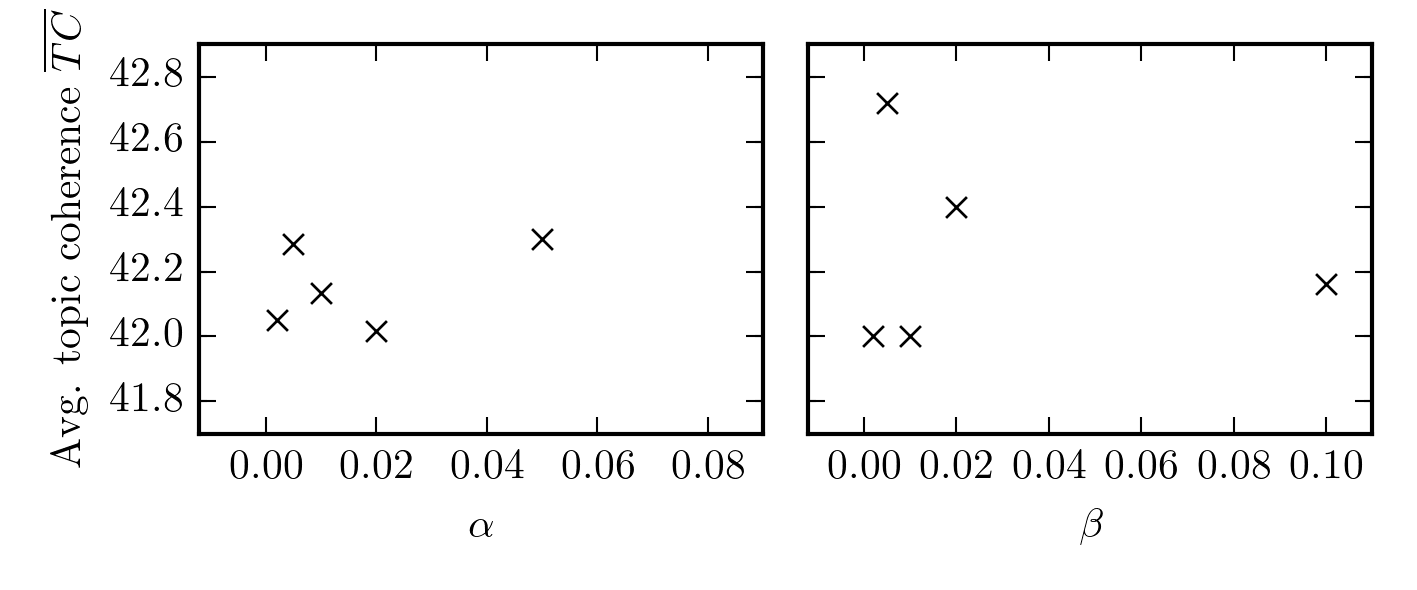
\includegraphics[width=12cm]{figures/standard_lda_alpha_beta.png}
       \caption{Average topic coherence for a fixed $\alpha$ respectively $\beta$, while averaging over all values of $\beta$ respectively $\alpha$. There is no trend recognizable, only random fluctuations. Therefore, $\alpha$ and $\beta$ have no influence on the topic coherence.}
       \label{fig:standard_lda_alpha_beta}
\end{figure}
As a baseline, we started with evaluating the topic coherence $TC$ of the standard LDA algorithm on the \textsc{20News} corpus.
We also used this to determine good values for the LDA parameters $\alpha$ and $\beta$.
We ran a grid search using $[0.002, 0.005, 0.01, 0.02, 0.05]$ as possible values for $\alpha$ and $[0.002, 0.005, 0.01, 0.02, 0.05, 0.1]$ as possible values for $\beta$.
Interestingly, there is no clear trend visible.
The best topic coherence results were achieved with $(\alpha=0.01,\beta=0.02)$, $(\alpha=0.005,\beta=0.005)$ and $(\alpha=0.02,\beta=0.1)$.
However, all results were in a very close range, with a standard deviation of all results of $0.6$, indicating no relationship between $\alpha$, $\beta$ and the topic coherence.
This impression is further strengthened by Figure~\ref{fig:standard_lda_alpha_beta}, where we plot the average topic coherence for a fixed $\alpha$ respectively $\beta$.
Again, no trend is recognizable.
Because of this observation, we fix our $\alpha$ and $\beta$ values for the following experiments on $\alpha = \beta = 0.02$.
The baseline topic coherence score for this parameter setting is $TC = 41.9$.
We show the development of the topic coherence through the Gibbs sampling iterations in Figure~\ref{fig:lda_20news_tc_development}.

The results are similar for the \textsc{Nips} corpus.
We again choose $\alpha = \beta = 0.02$ and start with a topic coherence baseline of $TC = 40.6$.

\begin{figure}
       \centering
       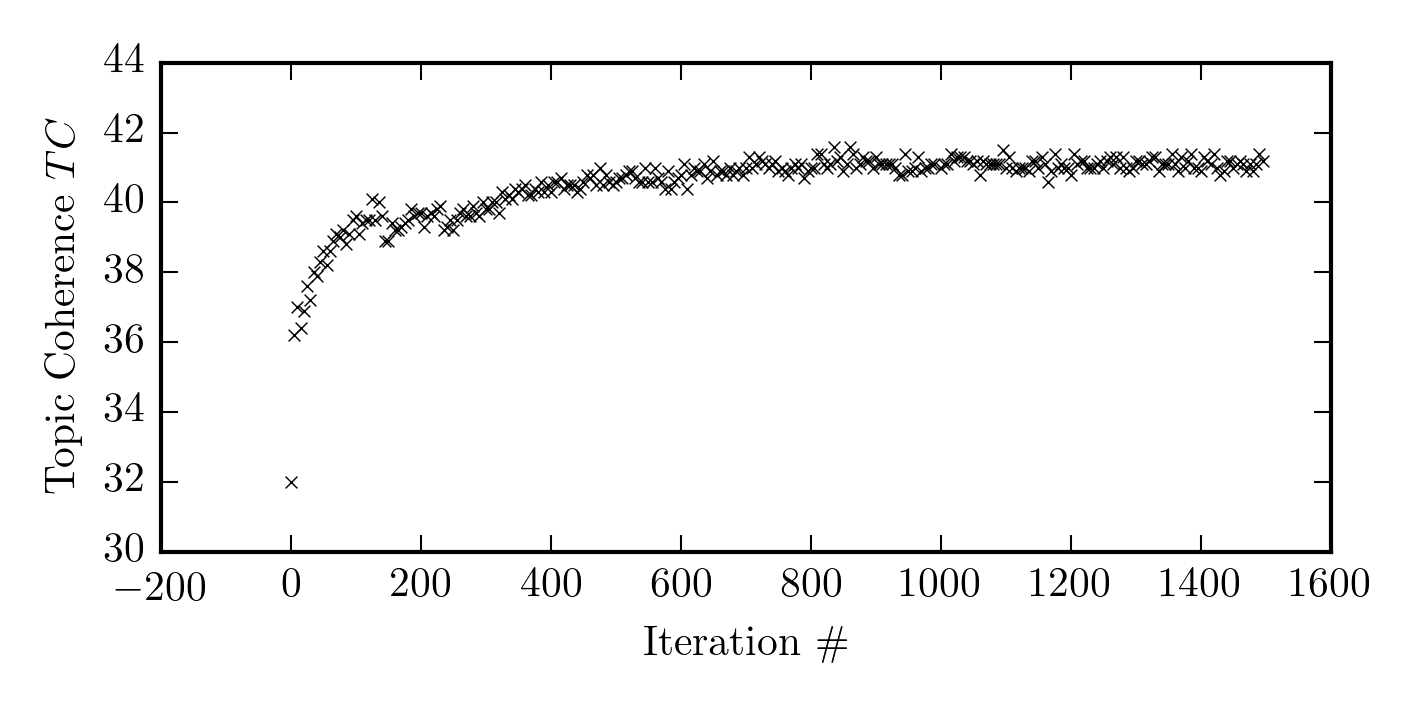
\includegraphics[width=12cm]{figures/lda_20news_tc_development.png}
       \caption{Development of the topic coherence for LDA on the \textsc{20News} corpus. The highest improvements occur in the first 200 iterations. After iteration 800, the topic coherence is constant except of random fluctuations.}
       \label{fig:lda_20news_tc_development}
\end{figure}

\subsubsection{Random fluctuations in WELDA}

As seen in the last section, the topic coherence of an LDA model is subject to random fluctuations.
This can be explained by the random component of LDA in the innermost loop of the Gibbs sampling, where new topics are sampled.
Due to the additional coin flip and the random sampling from the embedding space, WELDA is even more subject to random fluctuations in several runs.

Therefore, we evaluated how much the topic coherence fluctuates for several WELDA runs with the same parameter settings.
We ran ten identical experiments with $\lambda = 0.3$ on the \textsc{20News} corpus.
With corpus-specific embeddings, the $C_V$ value ranged from $44.8$ to $45.5$, with an average of $45.02$ and a standard deviation of $0.27$.
With Wikipedia embeddings, the $C_V$ value ranged from $44.5$ to $45.1$, with an average of $44.74$ and a standard deviation of $0.22$.
Because of this random fluctuations, it is best to rerun the model several times and pick the best.
In the following experiments, we ran each parameter setting three times.


\subsubsection{Influence of the resampling parameter $\lambda$}
We started the evaluation with the influence of the $\lambda$ parameter.
It must be noted, that the $\lambda$ parameter the algorithm is configured with at the beginning, is not the final $\lambda$ parameter.
This is because in addition to resampling when the coin flip succeeds, we also resample when corpus-specific stop words occur, that were identified from the background topic.
The plots in the following sections always use the actual $\lambda$, which we call $\lambda_{act}$.
This variable represents how often a word was replaced during sampling, either because it was a background word or because the coin toss was successful.
The $\lambda_{act}$ values are slightly higher than the original $\lambda$ values, with diminishing differences for higher $\lambda$. See Table~\ref{table:actual_lambda} for the differences.
\begin{table}[]
  \ra{1.2}
  \centering
  \caption{Comparison of $\lambda$ and $\lambda_{act}$. $\lambda_{act}$ is always greater than $\lambda$ with diminishing differences for higher $\lambda$}
  \label{table:actual_lambda}
  \begin{tabular}{lrrrrrrrrrrrr}
    \toprule
    $\lambda$     & 0.00 & 0.001 & 0.10  & 0.20  & 0.30  & 0.40  & 0.50  & 0.60  & 0.70  & 0.80  & 0.90  & 1.00 \\
    $\lambda_{act}$ & 0.00 & 0.11  & 0.20 & 0.29 & 0.38 & 0.46 & 0.55 & 0.64 & 0.73 & 0.82 & 0.91 & 1.00 \\
    \bottomrule
  \end{tabular}
\end{table}

\begin{figure}
       \centering
       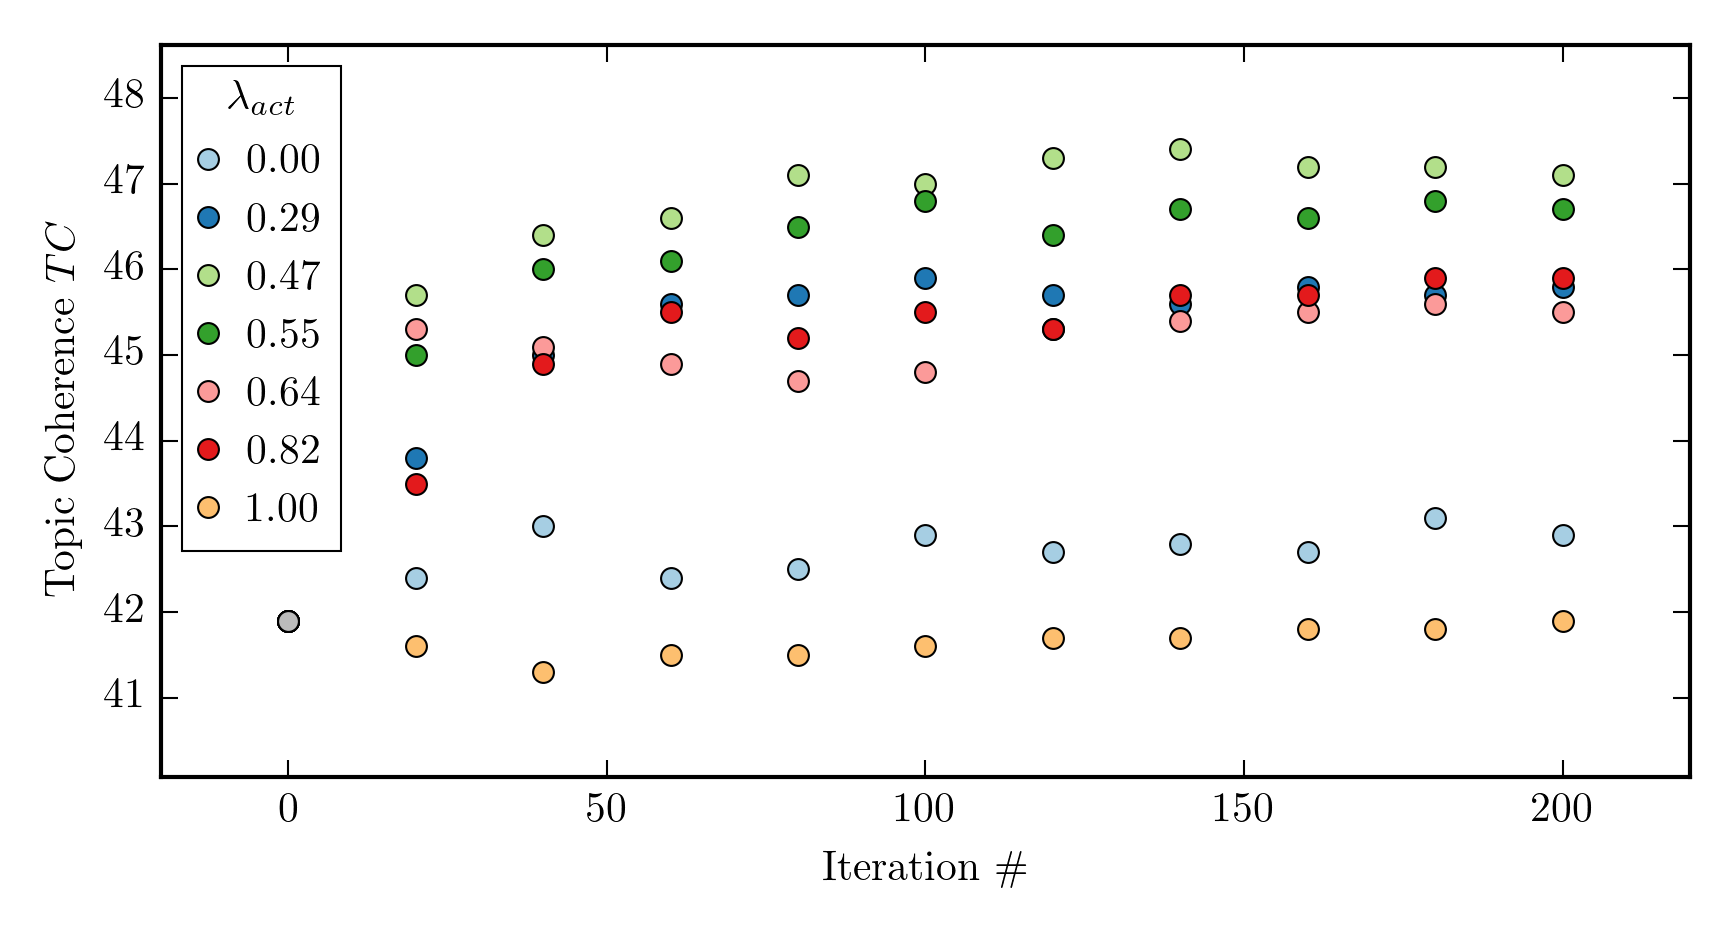
\includegraphics[width=\textwidth]{figures/welda_gaussian_lambda_20news.png}
       \caption{Gaussian WELDA's topic coherence development for different $\lambda_{act}$ values with \textsc{20News} as embedding corpus.
       Best results are achieved with $\lambda_{act} = 0.47$.}
       \label{fig:welda_gaussian_lambda_20news}
\end{figure}

% \printinunitsof{cm}\prntlen{\textwidth}
We start with the analysis of the topic models using the embeddings trained on the \textsc{20News} corpus.
We tested with $\lambda \in \{ 0.0, 0.2, 0.4, 0.5, 0.6, 0.8, 1.0 \}$.
The results with the corresponding $\lambda_{act}$ values in the legend are plotted in Figure~\ref{fig:welda_gaussian_lambda_20news}.
All runs start with the same value $TC = 41.9$ at iteration 0, because the models are initialized with the topic assignments from LDA.
For $\lambda = 0.0$ the topic coherence does not change afterwards except of random fluctuations.
This behaviour is expected, as WELDA with no replacement corresponds to standard LDA.
The same low topic coherence values can be observed when $\lambda = 1.0$, i.e. when all words are replaced.
This observation indicates, that just relying on the word embeddings to achieve good topics and completely disregarding the standard LDA structure, does not work.
Intuitively, when all words are resampled, the means of the topics roughly stay the same after each iteration, as no knowledge from the text is incorporated into the model anymore.
This results in roughly constant values for $\lambda = 1.0$.
Also see Section~\ref{sec:raw_tm_we}, where we experiment with a topic model solely based on word embeddings.

All the other $\lambda$ parameters follow a rising trend.
Especially the huge improvement from $\lambda_{act} = 0.0$ to $\lambda_{act} = 0.29$ shows, that the base idea of resampling words during the Gibbs sampling works.
The values tend to reach their optimum around iteration $140$ and stay there except some random fluctuations.
The best topic coherence value is reached with $\lambda_{act} = 0.47$ with a topic coherence of $47.4$.
Topic coherence values less than or greater than this $\lambda_{act}$ lead to worse topic coherence, which indicates that this value achieves a good balance between topic model and word embeddings.
All together, this is an improvement of $5.1$ over the baseline value.

We now compare the results from above with the results when we run WELDA with embeddings trained on Wikipedia.
We show the same plot as above for Wikipedia embeddings in Figure~\ref{fig:welda_gaussian_lambda_200}.
Interestingly, the topic coherence values are lower on average when using this embeddings.
This observation goes against the intuition, because topic coherence is evaluated using Wikipedia as a reference corpus.
One would expect, that knowledge from the Wikipedia corpus leaks into the topics during resampling and thus leads to better topic models.
However, this is not the case.
The observations for $\lambda_{act} = 0.0$ and $\lambda_{act} = 1.0$ are the same as above.
However, the same phanomenon as for $\lambda_{act} = 1.0$ here also occurs already for $\lambda_{act} = 0.82$.
The reason for this is the same as above: resampling too often throws away the corpus and just operates on the embeddings.
The best results with this embeddings is only $45.8$ as compared to $47.4$ with the corpus-specific embeddings.
This is only an improvement of $3.9$ over the baseline value.

\begin{figure}
       \centering
       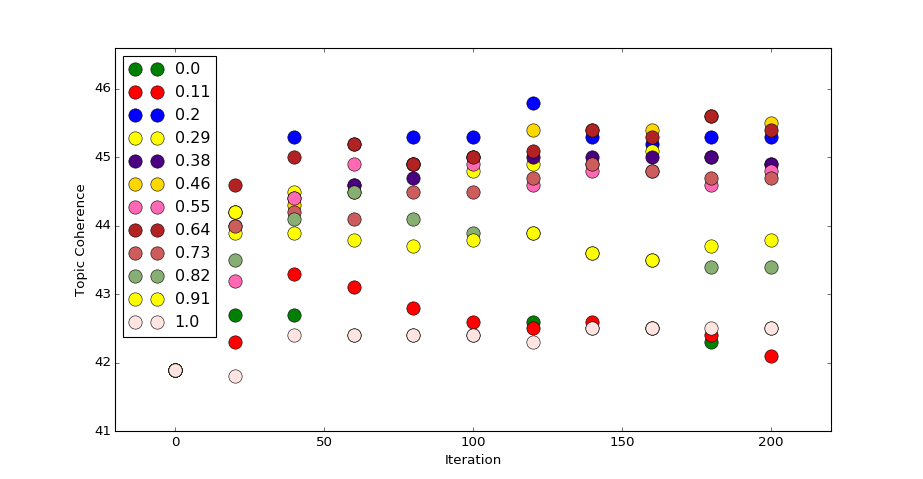
\includegraphics[width=\textwidth]{figures/welda_gaussian_lambda_200.png}
       \caption{Gaussian WELDA's topic coherence development for different $\lambda_{act}$ values with Wikipedia as embedding corpus. The topic coherence is lower than with corpus-specific embeddings. The best result is achieved with $\lambda_{act} = 0.47$ again.}
       \label{fig:welda_gaussian_lambda_200}
\end{figure}

The results for the \textsc{Nips} corpus are similar to the \textsc{20News} corpus regarding the best $\lambda$ values.
Medium $\lambda_{act}$ values between $0.4$ and $0.6$ produce the best results.
With corpus-specific embeddings, the maximum is reached at $TC = 42.2$, yielding an improvement of $1.3$ over the baseline.
This is different to the \textsc{20News} corpus, where the difference to the baseline was higher.
Also contrary to the \textsc{20News} corpus, the results on the \textsc{Nips} corpus are similar with Wikipedia embeddings.
The best value with Wikipedia embeddings is $TC = 42.4$.
These findings answer the initial question, on which type of corpus WELDA works better: the general \textsc{20News} corpus as opposed to the narrow, technical \textsc{Nips} corpus.
When the focus is narrow, many top topic words are close in the embedding space, therefore many topic distributions are similar.
Because of this, WELDA is not able to produce words, which clearly distinguish different topics during the resampling.
The respective graphs for the topic coherence development for different $\lambda$'s on the \textsc{Nips} corpus can be seen in Appendix~\ref{sec:appendix_nips_lambda}.

Finally, we give a qualitative overview over WELDA's topics.
In Table~\ref{table:topic_development}, we illustrate the change of topics in \textsc{Nips} and \textsc{20News} before and after WELDA iterations.
For both corpora, we picked the best model from above and compared it to standard LDA's topics.

\begin{table}[]
  \ra{1.15}
  \centering
  \caption{Topic evolution from standard LDA to Gaussian WELDA after 200 iterations. The crossed out words were in the original top ten words of LDA, but are not in the top topic words after WELDA. The bold words are the new words. The top three topics are from the \textsc{20News} corpus, the lower three from the \textsc{Nips} corpus. The examples clearly show WELDA's capability to add specific, meaningful words in the top words, while at the same time removing overly general words.}
  \label{table:topic_development}
  \begin{tabular}{p{13.5cm}}
    \toprule
    god \sout{believe} \sout{one} evidence religion \sout{people} argument exist \sout{question} atheists \textbf{faith belief existence life} \\
    year players baseball \sout{article} \sout{good} \sout{writes} lopez \sout{jewish} league average \textbf{hit braves season hitter} \\
    information list mail \sout{may} internet send anonymous \sout{faq} email \sout{use} \textbf{system available privacy} \\
    \midrule
    speech recognition speaker gamma acoustic phoneme \sout{time} vowel \sout{information} speakers \textbf{spectral phonetic} \\
    bayesian gaussian distribution prior posterior \sout{data} \sout{using} evidence \sout{mean} \sout{sampling} \textbf{random covariance monte carlo} \\
    kernel algorithm vector support loss margin \sout{set} \sout{function} linear examples \textbf{svm boosting} \\
    \bottomrule
    % \hline
  \end{tabular}
\end{table}

\subsubsection{Influence of the parameters $N_{pca}$ and $N_{top}$}

We will evaluate the influence of the parameters $N_{pca}$ and $N_{top}$ together in this section, as these parameters depend on each other.
$N_{pca}$ represents to which dimensionality we project the word embeddings using principal component analysis.
$N_{top}$ represents the number of top words in a topic used for estimating the topic distributions.
The larger $N_{pca}$ the larger $N_{top}$ needs to be, i.e. $N_{top} \geq N_{pca}$.
We conducted experiments with $\lambda = 0.5$ and the 200-dimensional Wikipedia embeddings on the \textsc{20News} corpus.
We illustrate the results in Figure~\ref{fig:welda_gaussian_pca_samples}.
We plot the development of the topic coherence with different fixed values of $N_{pca}$ against $N_{top}$.
The first observation is, that $N_{top}$ does not have a large influence on the topic coherence.
The regression is almost constant for all values of $N_{pca}$.
However, large differences are visible for different values of $N_{pca}$.
In general, the higher the value, the higher the topic coherence.
The exception to this observation is $N_{pca} = 2$, which performs better than $N_{pca} = 10$.
It seems that the first two dimensions encode already a lot information for WELDA.
Still, in general the trend shows higher topic coherence for higher values of $N_{pca}$ with a strong positive correlation.
For fixed $N_{top} = 200$, the correlation between $N_{pca}$ and $TC$ is $r_{Pearson} = 0.91$.
This observation can be explained, as dimensionality reduction always loses information.
With more dimensions more semantic information can be encoded in the embedding space and the similarity function between two words becomes more accurate.
We illustrate this in Figure~\ref{fig:embedding_model_dimensions_vs_similarity_corr} in Appendix~\ref{sec:embedding_model_dimensions_vs_similarity_corr}.
There, we project the Wikipedia embeddings to less dimensions using principal component analysis and then evaluate the word similarity correlation with human ratings from the \textsc{WordSim-353}~\cite{Agirre2009} data set.
There is a clear trend towards higher correlation with more dimensions.
The same experiment on the \textsc{Nips} corpus can be seen in Figure~\ref{fig:welda_gaussian_nips_pca_samples} in Appendix~\ref{sec:appendix_welda_gaussian_nips_pca_samples}.
The results are similar.

\begin{figure}
       \centering
       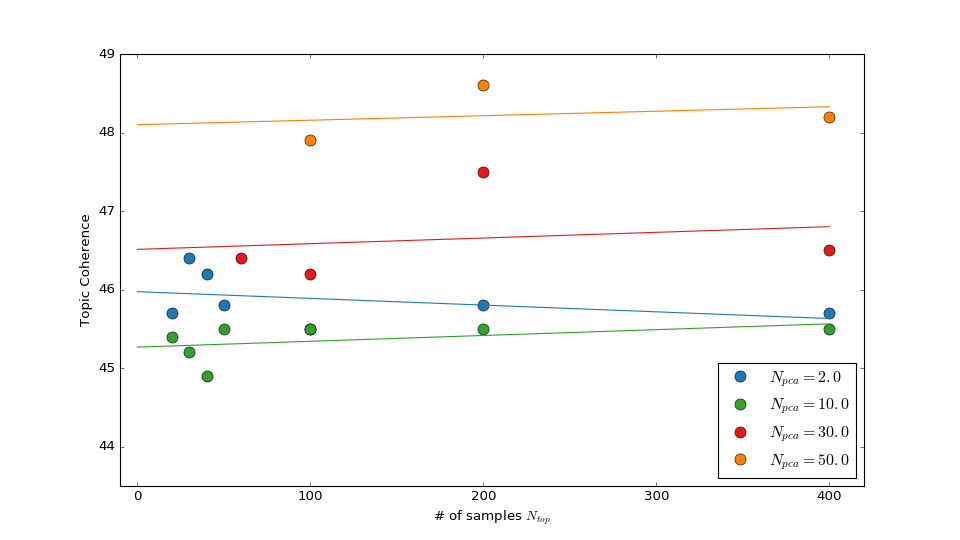
\includegraphics[width=\textwidth]{figures/welda_gaussian_pca_samples.png}
       \caption{Final topic coherence values after 200 iterations for different values of $N_{pca}$ and $N_{top}$. We also plotted a regression line indicating the development for increasing $N_{top}$. $N_{top}$ does not have a huge influence on the topic coherence. In contrast, the higher $N_{pca}$ the better the topic coherence.}
       \label{fig:welda_gaussian_pca_samples}
\end{figure}


\subsubsection{Influence of the background topic sampling}

We will now analyze the influence of the background topic.
When using background topic sampling, we also replace every occurrence of one of the top thirty words in the background topic in addition to all words, which had a successful coin flip.
When we replace these background words, the $\lambda$ is not equal to the actual $\lambda_{act}$, as we replace more words in that case.
When we do not use background topic sampling, the $\lambda$ is equal to $\lambda_{act}$.
We tested the influence of the background topic with $\lambda_{act} = 0.2$ and $\lambda_{act} = 0.5$.
To ensure similar $\lambda_{act}$ values with and without using background word sampling and to not influence the results by different $\lambda$ values, we tested different $\lambda$ parameters.
After some experiments, we found $\lambda = 0.10$ and $\lambda = 0.45$ to result in $\lambda_{act} = 0.2$ and $\lambda_{act} = 0.5$ when using background sampling.
Experiments were conducted on the \textsc{20News} corpus with Wikipedia embeddings.

Figure~\ref{fig:welda_gaussian_background_topic} confirms both facts of our initial hypothesis (see Section~\ref{sec:background_topic}).
First, using background word resampling leads to a faster convergence of the topic coherence.
The process is accelerated.
Second, similar topic coherence values are achieved in the end, as WELDA naturally replaces the often-occuring words more often.

\begin{figure}
       \centering
       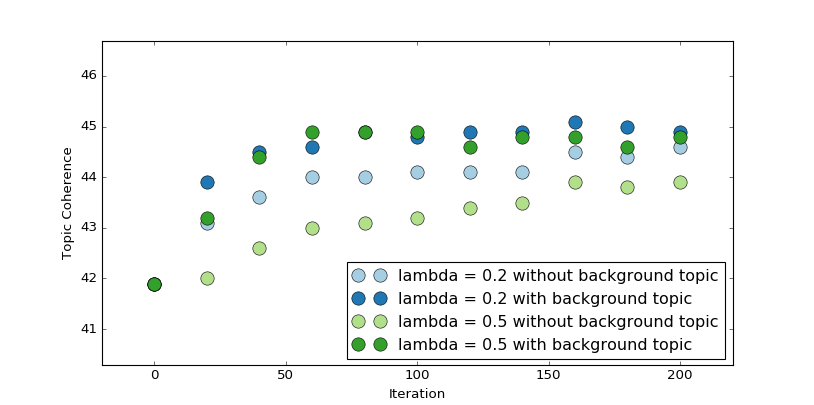
\includegraphics[width=\textwidth]{figures/welda_gaussian_background_topic.png}
       \caption{Comparison of WELDA with and without background topic. Background topic resampling converges faster, but not better.}
       \label{fig:welda_gaussian_background_topic}
\end{figure}

\subsubsection{Running LDA as a prerequisite}

We run standard LDA before WELDA to estimate the topic distributions on already well-defined topics.
We now evalute the performance of WELDA, when we initialize topics randomly as standard LDA.
This initial setup has a topic coherence value of $TC = 31.1$.
As convergence takes longer with random initialization, we ran WELDA for $1500$ iterations on \textsc{20News} with $\lambda = 0.5$.
As expected, WELDA performs far worse than before, reaching only $TC = 39.1$ with corpus-specific and $TC = 40.0$ with Wikipedia embeddings.



With random initialization, WELDA is actually harmful, as we do not even reach standard LDA's topic coherence of $TC = 41.9$.
The topic coherence development during the $1500$ iterations is displayed in Figure~\ref{fig:standard_lda_as_prerequisite} in Appendix~\ref{sec:appendix_lda_prerequisite}.
% \subsubsection{Strange behaviour for $\lambda_{act} = 1.0$} TODO
% When the words are spread far apart and the mean is in the middle of nowhere, things tend to overfit.
% /data/wikipedia/2016-06-21/topic-models/topic.20news.50-1500.alpha-0-02.beta-0-02/model.20news.dim-50.skip-gram.embedding.welda.gaussian.distance-cos.lambda-1-0/welda.iteration-200.topics

\subsubsection{WELDA with von Mises-Fisher distributions}

So far, all experiments were executed with Gaussian distributions as the topic distributions.
We now evaluate WELDA with von Mises-Fisher distributions (vMF).
We conducted experiments on the \textsc{20News} corpus with $N_{pca} = 10$ and $N_{top} = 20$.
The results and the differences to Gaussian WELDA are displayed in Table~\ref{table:welda_vmf}.
In Appendix~\ref{sec:appendix_welda_vmf}, we also show the plots for the topic coherence development through the iterations.
Interestingly, the results are different depending on the embedding used.
WELDA vMF performs worse than Gaussian WELDA when using corpus-specific embeddings.

\begin{table}[]
  \ra{1.3}
  \centering
  \caption{Comparison of WELDA's topic coherence with Gaussian distributions and with von Mises-Fisher (vMF) distributions on \textsc{20News}. The $\Delta TC$ columns indicate the difference. A negative value indicates that von Mises-Fisher distributions perform worse.}
  \label{table:welda_vmf}
  \begin{tabular}{@{}ccccccc@{}}
    \toprule
                     &                 & \multicolumn{2}{c}{\textsc{20News}} && \multicolumn{2}{c}{Wikipedia} \\
           \cmidrule{3-4} \cmidrule{6-7}
           $\lambda$ & $\lambda_{act}$ & $TC~vMF$        & $TC~GM$ &           & $TC~vMF$         & $TC~GM$      \\
           \midrule
           0.2       & 0.29            & 45.8 $\pm 0.0$  & 46.0 $+0.2$    && 46.1   $+1.1$  & 45.0 $\pm 0.0$ \\
           0.4       & 0.47            & 45.3 $-1.8$     & 45.7 $-1.4$    && 45.9   $+0.3$  & 44.7 $-0.9$     \\
           0.5       & 0.56            & 45.6 $-1.1$     & 46.0 $-0.7$    && 46.0   $+0.5$  & 44.8 $-0.7$     \\
           0.6       & 0.64            & 45.1 $-0.4$     & 44.8 $-0.7$    && 45.6   $+0.8$  & 45.5 $+0.7$     \\
           0.8       & 0.82            & 45.0 $-0.9$     & 44.5 $-1.4$    && 44.8   $+1.4$  & 44.3 $+0.9$     \\ \bottomrule
           % some of these were run with 300 iterations, see welda-vmf-longer.log
                     % &                 & \multicolumn{4}{c}{\textsc{20News}} && \multicolumn{4}{c}{Wikipedia} \\ \cmidrule{3-6} \cmidrule{8-11}
           % $\lambda$ & $\lambda_{act}$ & $TC~vMF$             & $\Delta TC$ & $TC~GM$             & $\Delta TC GM$ &          & $TC~vMF$   & $\Delta TC vMF$ & $TC~GM$  & $\Delta TC GM$      \\
  \end{tabular}
\end{table}


\section{Document classification}
We also evaluated topic models on another commonly used task: document classification.
In contrast to topic coherence, this allows to use topic models in an supervised setting with clear evaluation metrics.
Given a set of documents, which belong to different semantic groups, the task of document classification is to correctly classify unseen documents into these groups.

We use the document-topic matrices.

\subsection{Experiment setup}
\subsection{Results}


\chapter{Comparative evaluation of word-embedding-improved topic models}
\label{sec:comparative_evaluation}

In this chapter, we will evaluate WELDA in comparison to TopicVec, Gaussian LDA, LFTM, NSTM and standard LDA.
We will focus on two tasks: topic coherence and document classification.

\section{Topic coherence}
\label{sec:evaluation_topic_coherence}

We will now evaluate topic coherence as described in Section~\ref{sec:topic_coherence} on all models.

\subsection{Topic model solely based on word embeddings}
\label{sec:raw_tm_we}
As a baseline, we start with a topic model solely based on the word-similarity in the embedding space.
This way, we see whether using the most similar words for a given word already yields good topics, or whether standard LDA is still important for creating good topics.

For this, we used the standard \emph{distance} function, that is provided in the word2vec implementation.
Given a word, this outputs the top $n$ similar words in the embedding space.
Given a list of words, the corresponding word vectors are averaged first and then the most similar words in the embedding space are retrieved.
In the original implementation, the search words are never in the output.
We modified this, so that the search words may also be in the output.
For one search word, the search word is always in the output, as the similarity is $1$.

As search words, we took the top topic words of a standard LDA run with $iterations=1500, \alpha=0.02, \beta=0.02$.
We experimented with two cases: only taking the top word and taking the average of all top ten words.
For example, for the search word ``game'', the topic (in the 200-dimensional embeddings trained on Wikipedia) is:
\topicbox{\noindent game games skullgirls tetris gameplay battletoads puzzle 2player picross multiplayer}

We show the results in Table~\ref{table:raw_we_tm}.
The results are worse than running LDA, thus showing that only using word embeddings is not enough.
The information contained in the bag-of-words and exploited by LDA is still crucial for good topics.
\begin{table}[]
  \ra{1.3}
  \centering
  \caption{Topic coherence on the \textsc{20News} corpus when using word embedding similarity for topics. The results are slightly worse than standard LDA.}
  \label{table:raw_we_tm}
  \begin{tabular}{ccc}
    \toprule
    search word     & 200-dim., \textsc{Wikipedia} & 50-dim., \textsc{20News} \\
    \midrule
    top word                 & 0.414                        & 0.410                    \\
    average of top ten words & 0.419                        & 0.389 \\
    \bottomrule
  \end{tabular}
\end{table}

\subsection{Contenders}
We now present the different settings for the contenders.

\begin{itemize}
  \item
    \textbf{Standard LDA:}
    We ran LDA with different values of $\alpha$ and $\beta$.
    However, there is no influence of these parameters on the classification results.
    We report the results for $\alpha = \beta = 0.02$ and use the same values in the other methods, if applicable.
  \item
    \textbf{Gaussian LDA:}
    Compared to the other methods, Gaussian LDA had to be trained with 50-dimensional instead of 200-dimensional word embeddings trained on Wikipedia.
    When training with higher-dimensional embeddings, Gaussian LDA does not converge and yield recognizable topics.
    We could confirm this issue in communication with the authors~\cite{Das2016}.
  \item
    \textbf{LFTM:}
    We report results for LFTM with $\lambda = 1.0$, as this yields the best topic coherence results according to the original paper.
    We could confirm this in our experiments.
    With $\lambda = 1.0$ every word is sampled from the embedding space and the multinomial word-distribution from standard LDA is effectively discarded.
  \item
    \textbf{NSTM:}
    We had the same problems with NSTM as with Gaussian LDA: training with 200-dimensional embeddings did not succeed.
    We could confirm these issues in communication with the authors~\cite{Saeedi2016}.
    Thus, we again used the 50-dimensional embeddings.
    For the \textsc{20News} corpus, we could still could not obtain any results.
    We only report the results for the \textsc{Nips} corpus.
    We preprocessed all word embeddings to have unit norm, as the von Mises-Fisher distribution in NSTM places probability mass only on the hyper-sphere.
  \item
    \textbf{TopicVec:}
    The authors did not evaluate the performance of TopicVec with topic coherence, so no best parameter settings are given.
    The relevant parameters are the learning rate $\delta$ and the hypersphere radius $\gamma$.
    We experimented with $\delta \in \{ 0.01, 0.05, 0.1, 0.2, 1.0 \}$ and $\gamma \in \{ 1, 5, 7, 10 \}$.
    Best results were achieved with $\delta = 0.1$ and $\gamma = 7$, which are also the values reported in the paper for document classification.
    In contrast to the other methods, TopicVec needs different preprocessing, as it is trained on the context of a word, similarily to the skip-gram architecture for word-embeddings.
    Therefore, we do not lowercase the text and do not remove stop words.
    The text is tokenized into sentences, as TopicVec processes one sentence at a time.
    We trained for 500 iterations.
  \item
    \textbf{WELDA:}
    TODO
\end{itemize}

To eliminate random effects, we ran all methods with the best settings three times and report the best results.

\subsection{Results}
We show the results of the topic coherence experiments in Table~\ref{table:topic_coherence}.
The two best methods by far are WELDA and TopicVec.


The two remaining methods, Gaussian LDA and NSTM, perform even worse than standard LDA.

\begin{table}[]
  \ra{1.3}
  \centering
  \caption{Topic coherence on the \textsc{20News} and \textsc{Nips} corpus. The }
  \label{table:topic_coherence}
  \begin{tabular}{@{}lrrcrr@{}}
    \toprule
                 \multicolumn{1}{r}{Corpus:} & \multicolumn{2}{c}{\textsc{20News}} && \multicolumn{2}{c}{\textsc{Nips}} \\ \cmidrule{2-3} \cmidrule{5-6}
                 \multicolumn{1}{r}{Embeddings:}  & Wikipedia     & \textsc{20News}     && Wikipedia     & \textsc{Nips}     \\
                 \midrule
                              LDA          & \multicolumn{2}{c}{41.9}   && \multicolumn{2}{c}{40.6} \\
                              Gaussian LDA & 38.5          & 40.3       && 39.2          & 39.5     \\
                              LFTM         & 43.9          & 45.6       && 41.6          & 43.5     \\
                              NSTM         & --            & --         && 37.5          & 36.8     \\
                              TopicVec     & 48.5          & 46.2       && 43.4          & 43.6     \\
                              WELDA        & TODO          &            &&               &          \\
                              \bottomrule
  \end{tabular}
\end{table}

\section{Document classification}

To investigate the effects of the different word embedding-enhanced topic models on document classification, we conducted a series of experiments, which we will present in the next sections.

\subsection{Setup}

As features, we took the document-topic matrix: this matrix contains the distribution of topics in each topic.
Each row sums to one.
The number of features is equal to the number of topics.
We ran experiments for all approaches using $K = 50$ and $K = 250$.

For classification, we ran a three-fold stratified cross validation.
In each fold, we used a linear \emph{l}-1 regularized SVM classifier, where we trained $K$ one-vs-rest classifiers.
The results for the different classes were macro-averaged.
The results for the three folds were macro-averaged again.
We will report this number in the tables in the following sections.
We used the \emph{LinearSVC} implementation from the Python scikit-learn~\cite{Pedregosa2012} library.

Additionally, we wanted to analyze the effect of unmodified word embeddings for document classification.
For this, we conducted additional experiments, where we added the average word embedding of each document to the features.
The average was calculated by taking the bag-of-words representation of the documents from the topic model, retrieving all word vectors using the word-matching technique described in Section~\ref{sec:vocabulary_mismatch} and then calculating their average.
This means, that stop words were not relevant for the average calculation, as they were already removed during the topic model preprocessing.
Depending on the word embeddings used (see Table~\ref{table:word_embeddings_performance}), this added another fifty or two-hundred features to the instances.

\subsection{Contenders}

\begin{itemize}
  \item
    \textbf{Standard LDA:}
    We ran LDA with different values of $\alpha$ and $\beta$.
    However, there is no influence of this parameters on the classification results.
    We report the results for $\alpha = \beta = 0.02$ and use the same values in the other methods, if applicable.
  \item
    \textbf{TopicVec:}
    Contrary to the paper by Li et al.~\cite{Li2016}, we configured TopicVec to only learn one set of topics.
    In their paper, they learn 14 topics separately on each classification category and then combine them, resulting in 280 topics.
    However, to allow a fair comparison, we 
    The learning rate was set to $\delta = 0.1$, as they reported in the paper.
    We used the parameters they reported in their paper, 
  \item
    \textbf{Mean of word embeddings:}
    As a baseline, we also 
  \item
    \textbf{WELDA:}
    WELDA with lambda = 0.3
  \item
    \textbf{LFTM:}
    We report results for LFTM with $\lambda = 0.6$, as this yields the best document classification results according to the original paper.
    We could confirm this in our experiments.
  \item
    \textbf{Gaussian LDA:}
    Compared to the other methods, Gaussian LDA had to be trained with 50-dimensional instead of 200-dimensional word embeddings trained on Wikipedia.
    When training with higher-dimensional embeddings, Gaussian LDA does not converge and yield interpretable results~\cite{Das2016}.
    When adding the average word vector to the features, we still used the 200-dimensional Wikipedia embeddings.
\end{itemize}


\subsection{Results}

\begin{table}[]
  \ra{1.3}
  \centering
  \caption{Document classification results for the \textsc{20News} corpus when using 200-dimensional embeddings trained on Wikipedia.
  We tested with $K = 50$ topics and with $K = 250$ topics and report macro-averaged precision ($Prec$), recall ($Rec$) and F1 score ($F1$).
  All word-embedding-improved topic models perform worse than standard LDA.}
  \label{table:document_classification_dim-200}
  \begin{tabular}{lrrrcrrr}
    \toprule
    \multirow{2}{*}{} & \multicolumn{3}{c}{$K = 50$} & \phantom{a} & \multicolumn{3}{c}{$K = 250$} \\ \cmidrule{2-4} \cmidrule{6-8}
                      & $Prec$    & $Rec$     & $F1$     && $Prec$    & $Rec$   & $F1$     \\ \midrule
                      Only Avg. Emb. (200)     & 71.5    & 70.4    & 69.9   && \multicolumn{3}{l}{}        \\
                      Only Avg. Emb. (50)      & 57.3    & 58.3    & 56.7   && \multicolumn{3}{l}{}        \\
                      LDA                      & 71.1    & 71.2    & 70.1   && 73.2    & 72.8     & 72.6   \\
                      LDA + Avg. Emb.          & \textbf{76.5}    & \textbf{76.2}    & \textbf{77.0}   && \textbf{78.1}    & \textbf{77.7}     & \textbf{77.6}   \\
                      LFTM                     & 69.0    & 67.7    & 66.5   && 71.4    & 71.0     & 70.8   \\
                      LFTM + Avg. Emb.         & 74.6    & 74.5    & 73.9   && 77.4    & 77.0     & 76.9   \\
                      TopicVec                 & 34.7    & 34.4    & 31.4   && 40.9    & 37.3     & 33.7   \\
                      TopicVec + Avg. Emb.     & 74.2    & 73.1    & 72.1   && 74.3    & 73.4     & 72.5   \\
                      WELDA                    & 62.1    & 61.3    & 61.0   && 67.1    & 64.8     & 65.1   \\
                      WELDA + Avg. Emb.        & 73.4    & 73.2    & 72.7   && 76.8    & 76.5     & 76.3   \\
                      Gaussian LDA             & 41.6    & 43.4    & 40.5   && 40.3    & 42.5     & 39.1   \\
                      Gaussian LDA + Avg. Emb. & 72.7    & 72.3    & 71.8   && 68.0    & 68.9     & 67.8   \\
  \bottomrule
  \end{tabular}
\end{table}

The results for the different techniques with 200-dimensional Wikipedia embeddings are displayed in Table~\ref{table:document_classification_dim-200}.
As a baseline, the first row shows the performance of the average vector without any topic model features.
Already these features achieve an F1-score of 69.9 \%.
The other baseline we use is standard LDA, which achieves 70.1 \%, so already slightly more than the average word embeddings.
Combining the two baselines, i.e. taking standard LDA's document-topic matrix and the average word vector, yields the highest F1 score for both $K = 50$ and $K = 250$.
The scores are 77.0 \% and 77.6 \% respectively.
No other technique can beat standard LDA in the document classification task.
However, all methods at least can improve over the average word vector with their features.
TopicVec has the largest improvements when adding the average word embedding vector, however, it also had the worst results before.
When looking at the word-embedding-improved topic models without the average vector, LFTM fares best, followed by WELDA with 7 \% distance.
Gaussian LDA and TopicVec follow with a huge gap.
Especially, TopicVec shows a surprisingly low performance.
In their paper,  Li et al.~\cite{Li2016} train topics independently on each class and achieve comparatively best performance in their document classification tests.
We did not follow this methodology, because it leads to a different number of topics and we wanted to compare all methods in their standard setting.
It seems that most of its predictive power stems from this training approach.

In general, the F1 scores are higher for $K = 250$, with the exception of Gaussian LDA.
This can be explained, because more features are available and because the topic model can assign topic proportions on a more fine-grained level.
However, the improvement is only a few percent for all models.

We also tested all methods with embeddings, which were trained on the corpus itself.
The results with the 50-dimensional \textsc{20News} embeddings are displayed in Table~\ref{table:document_classification_dim-50} in Appendix~\ref{sec:appendix_document_classification_corpus_specific}.
Interestingly, the predictive power of the embeddings is already much higher than before, even though these embeddings failed in the analogy reasoning benchmark (see Table~\ref{table:word_embeddings_performance}).
The F1 score of these embeddings when only taking the average vector of each document is already 78.0 \%.
Also, all methods perform better with even without the average vector features compared to the 200-dimensional Wikipedia embeddings.
The comparatively low number of dimensions for word embeddings does not seem to do harm in this use case.

Especially LFTM profits from the different embeddings.
It is now able to surpass standard LDA for both $K = 50$ and $K = 250$, achieving the highest F1-score of 81.5 \% in all our document classification tests.
It is worth to note, that the raw LFTM topic model features does not perform better than LDA, but only when adding the average vector.
The order of the remaining methods is not different from before.
The same holds for the number of topics: $K = 250$ performs better than $K = 50$ for all models.

As a summary, using the word embeddings during the inference does not help to create better document representations.
While most methods were able to generate better topics (see Section~\ref{sec:evaluation_topic_coherence}), this seems to come at the expense of loosing accuracy in document classification.
However, in general, topic model features and word embedding features (in the form of the average vector) complement each other.
Both features combined are always better than just one of the two models.
Also, the fact that the average vector alone already has a high F1 score indicates, that word embeddings are well-suited for document classification in general.
The approaches just seem to not be able to use the knowledge in the embedding space properly.

\section{Word intrusion study}

So far, we evaluated the quality of our topics using the $C_V$ by Röder et al.~\cite{Roder2015}, which we introduced in Section~\ref{sec:topic_coherence}.
While this method is cheap and many models can be evaluated, the correlation with human ratings is not perfect, but only $r_{Pearson} = 0.731$.
Also, it is based on co-occurrence statistics from the English Wikipedia under the assumption, that this corpus contains a large number of topics and can therefore be used as a reference corpus.
In the case of the \textsc{20News} corpus with its wide range of general topics, this assumption holds.
However, it is questionable for the \textsc{Nips} corpus.
The \textsc{Nips} with its scientific papers and many technical terms has a clearly different scope.

For this reasons, we decided to conduct a manual study on the \textsc{Nips} corpus.
We evaluated the quality of a topic model by the word intrusion task by Chang et al.~\cite{Chang2009}.
In this task, a subject is presented with a list of six words.
Five of these six words belong to the top words of one topic of the topic model.
The sixth word is chosen randomly from another topic.
This word is called the \emph{intruder}.
Our potential intruders had to be in the top ten words of another topic, but not in the top fifty words of the topic the first five words stem from.
The word order is randomized.
The idea of this word intrusion study is the following: if the five words form a clear, coherent topic, it should be simple to detect the intruder.
For example, look at the word set:
\topicbox{gaussian bayesian posterior neural distribution prior}
The intruder ``neural'' is easily recognizable, because all other words stem from Bayesian statistics.
However, in the sample:
\topicbox{error generalization hypothesis convergence evidence probability}
the intruder ``convergence'' is much harder to recognize.
In this cases, the chance that the subject recognizes the wrong word is much lower.
The percentage of correctly identified intruders, the accuracy, is taken as the evaluation metric to assess the quality of a topic model.

In our study, we picked the four best models from Section~\ref{sec:evaluation_topic_coherence}, i.e. LDA, LFTM, TopicVec and WELDA.
We tested two different scenarios: one with $K = 50$ topics and one with $K = 20$ topics.
We created one sample for each topic.
This resulted in 200 samples for the 50-topic topic models and 80 samples for $K = 20$.
Our subject group consisted of computer science students and computer scientists familiar with the topics of the \textsc{Nips} corpus.
To not bias the results, subjects were not presented with the information, whether their selection was correct~\cite{Chang2009}.
Also, the underlying topic model was not displayed and we randomized the order of the samples.

We present the results in Figures~\ref{fig:word_intrusion_20} and \ref{fig:word_intrusion_50}.
For the plot, we calculated the accuracy of each subject on each topic model.
Each model was evaluated by at least five subjects, so we had at least five accuracy values.
We then plotted the distribution of the accuracy for each model.
For both $K = 20$ and $K = 50$ WELDA achieves the highest accuracy.

\begin{figure}
       \centering
       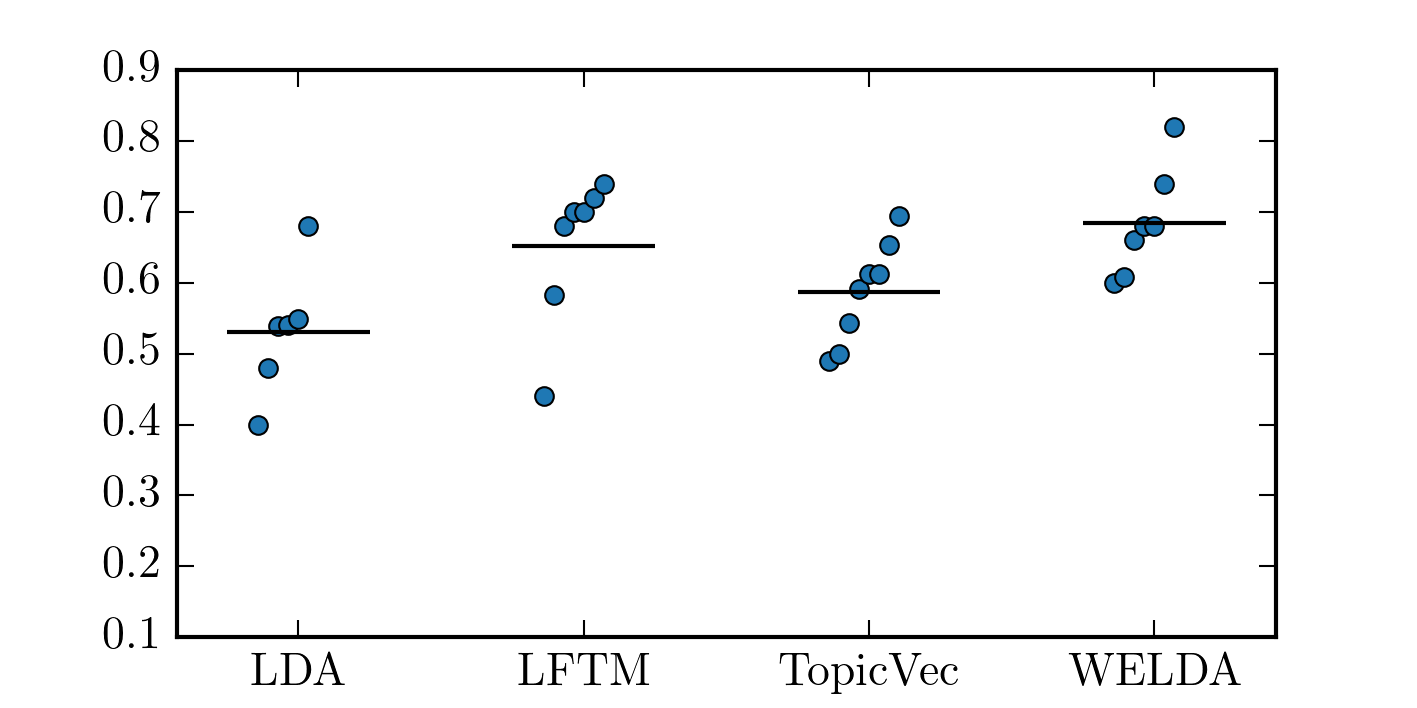
\includegraphics[width=12cm]{figures/word_intrusion_50.png}
       \caption{Word intrusion study results for 50 topics. The plot shows the distribution of the accuracy for all subjects. The red line indicates the median. WELDA achieves the highest accuracy.}
       \label{fig:word_intrusion_50}
\end{figure}

\begin{figure}
       \centering
       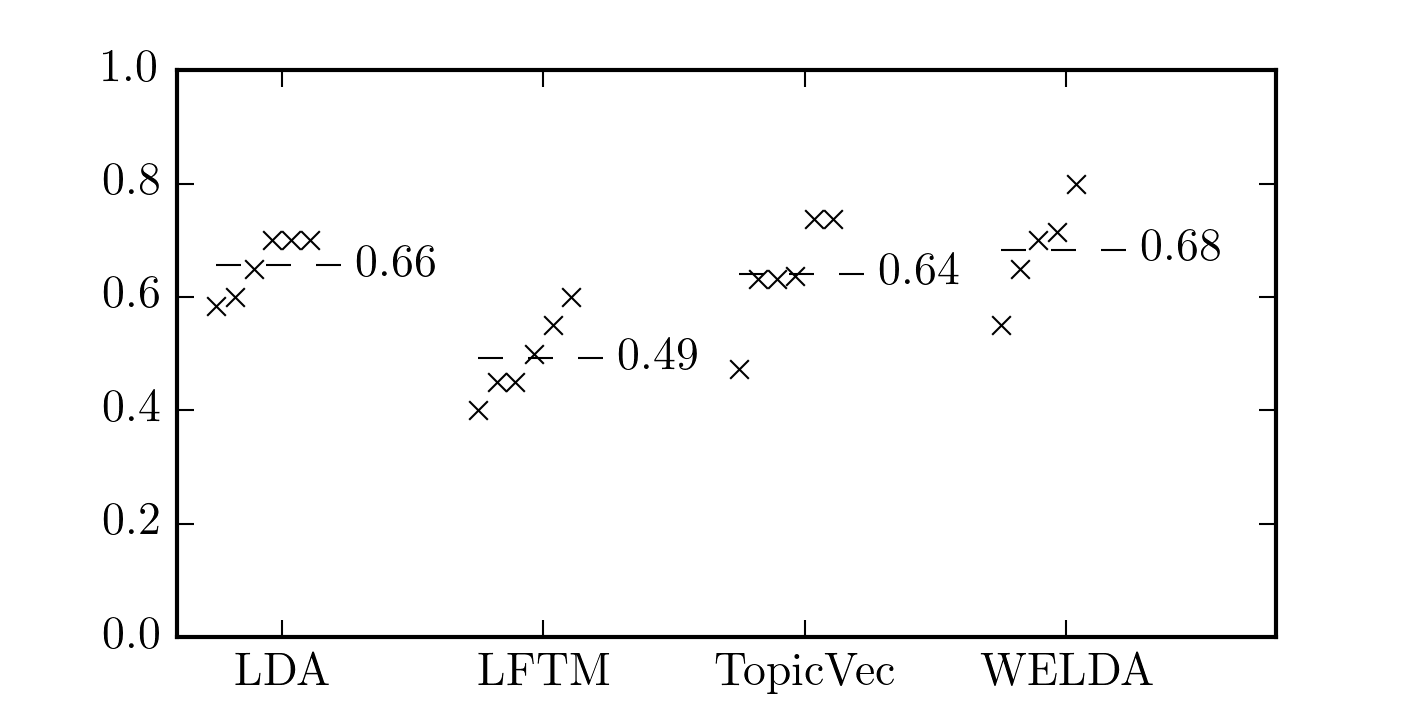
\includegraphics[width=12cm]{figures/word_intrusion_20.png}
       \caption{Word intrusion study results for 20 topics. WELDA achieves the highest accuracy.}
       \label{fig:word_intrusion_20}
\end{figure}

\section{Runtime}
\label{sec:runtime}

In this section we present the running time of the different algorithms.
Run time is not a crucial factor for topic models, as they are usually not executed in an online setting.
Still, to gain an impression on the computational complexity of each model, we present their runtimes here.

Experiments were conducted on a 32-core, Intel Xeon CPU E7-8837 @ 2.67GHz machine with 256 GB memory.
While same techniques have parallelized implementations available, other's have not.
To ensure comparability, we ran all techniques with only a single core.

We will now present the different implementations and also whether they can be parallelized.
For LDA, we ran the implementation in Mallet~\cite{McCallum2002}, which implements the approach by Newman et al.~\cite{Newman2009} for distributed LDA.
However, we will use only the single-threaded implementation, running for $1500$ iterations.
Mallet is the only highly optimized library in this benchmark.
The LFTM\footnote{\url{https://github.com/datquocnguyen/LFTM}} does not offer a parallelized implementation.
The only step, which is parallelized is the optimization of the topic vector, which happens after each Gibbs sampling iteration.
We ran LFTM for $500$ iterations, as suggested in the paper.
TopicVec\footnote{\url{https://github.com/askerlee/topicvec}} offers an parallel implementation, which mostly relies on existing parallelization in linear algebra libraries, as TopicVec heavily works with matrix operations.
We ran TopicVec for $500$ iterations.
Gaussian LDA\footnote{\url{https://github.com/rajarshd/Gaussian_LDA}} is not parallelized and no straightforward parallelization is possible.
Gaussian LDA was run for $150$ iterations,  which is when the log likelihood converges.
WELDA is not parallelized, however a parallel implementation with the same ideas as Newman et al.~\cite{Newman2009} is possible.
As usual, we run WELDA for $200$ iterations.

All methods were run until convergence.
% See the previous sections for details.
Of all methods, standard LDA is by far the fastest.
The next best method is WELDA, but it is already slower by a factor of ten.
Note that especially WELDA's performance largely depends on the resampling probability $\lambda$.
The higher $\lambda$, the more new words are sample, which leads to more nearest-neighbour searches.
The nearest-neighbour search is the most expensive operation, hence it dominates the runtime.
We illustrate this dependency in Figure~\ref{fig:welda_lambda_runtime}.
Still, even with $\lambda = 1.0$ the runtime of WELDA is 164 min, which is still faster than the next-fastest TopicVec.
Especially LFTM is very slow with 200-dimensional embeddings, making it infeasible to run on larger corpora.

\begin{table}[]
  \ra{1.2}
  \centering
  \caption{Runtimes of the different methods with $K = 50$ on the \textsc{20News} and \textsc{Nips} corpus.
  Experiments were conducted with the 200-dimensional Wikipedia embeddings for \textsc{20News} (50-dimensional for Gaussian LDA) and the 50-dimensional corpus-specific embeddings for \textsc{Nips}.
  }
  \label{table:runtime}
  \begin{tabular}{@{}lp{4cm}rr@{}}
    \toprule
                                    & Parallel implementation \newline available & \multicolumn{1}{c}{\textsc{20News}} & \multicolumn{1}{c}{\textsc{Nips}} \\
    \midrule
    LDA                             & ~~~~~~~~~~~~~~~~\cmark                     &    6 min                            &    9 min \\ % 378 seconds, 527 seconds
    LFTM, $\lambda = 0.6$           & ~~~~~~~~~~~~~~~~\xmark                     & 3672 min                            &   71 min \\
    TopicVec                        & ~~~~~~~~~~~~~~~~\cmark                     &  178 min                            &  116 min \\
    Gaussian LDA                    & ~~~~~~~~~~~~~~~~\xmark                     & 1403 min                            & 2880 min \\
    WELDA Gaussian, $\lambda = 0.5$ & ~~~~~~~~~~~~~~~~\xmark                     &   67 min                            & TODO \\  % 4027 sec,
    WELDA vMF, $\lambda = 0.5$      & ~~~~~~~~~~~~~~~~\xmark                     &  101 min                            & TODO \\ \bottomrule
  \end{tabular}
\end{table}

\begin{figure}
       \centering
       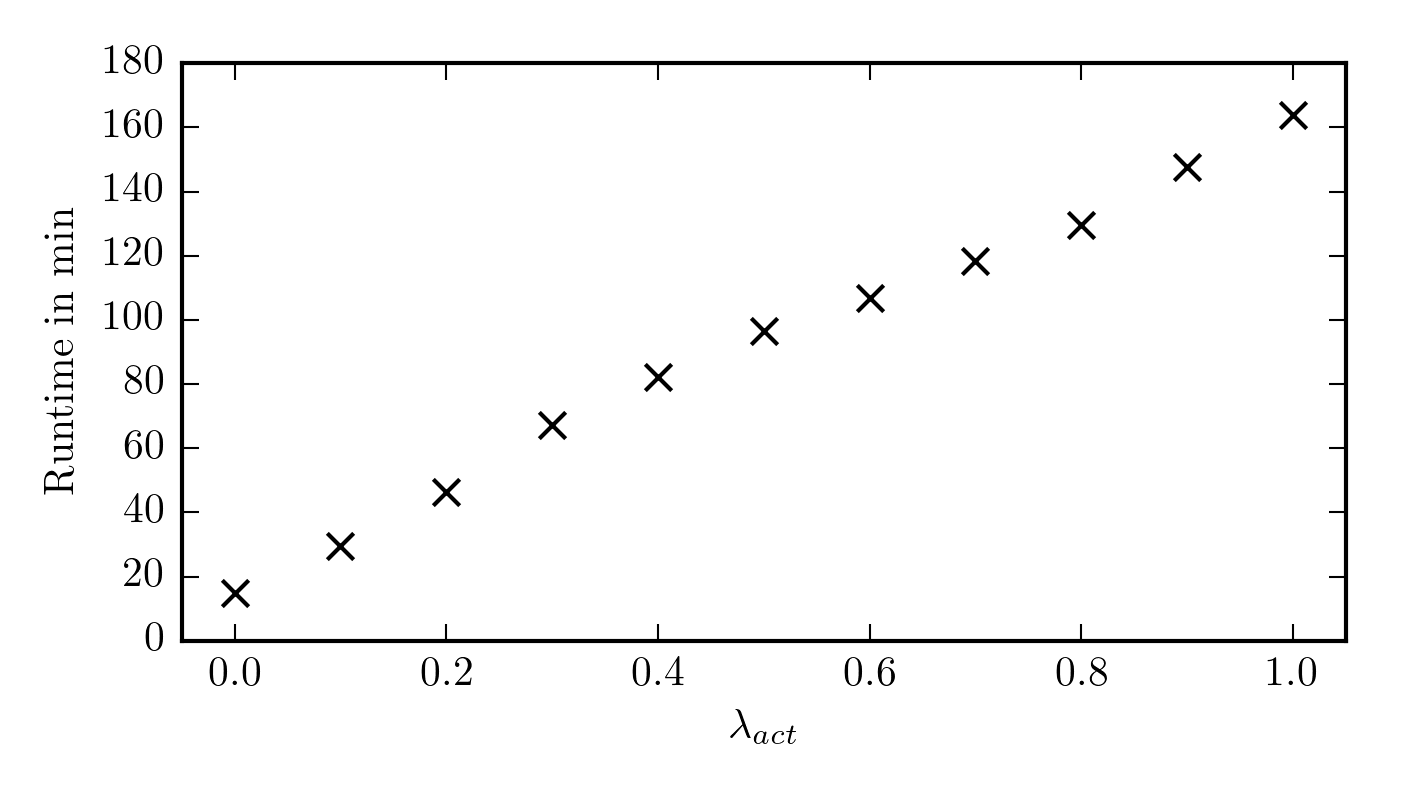
\includegraphics[width=0.9\textwidth]{figures/welda_lambda_runtime.png}
       \caption{Runtime of WELDA depending on the resampling parameter $\lambda$.}
       \label{fig:welda_lambda_runtime}
\end{figure}



\chapter{Conclusion and future work}
\label{sec:conclusion}

Document classification
Topic specific replacement

% \section{Other notes}
Concept categorization
Visualize in tsne

Hyperparameter optimization
Motivation: topic with countries
Paper: Schwächen, Stärken, ausführlich

Beim resampling: sanity check, ABER: optimiert auf, Wort nur in 1 topic
curse of dimensionality for nearest neighbour search
fewer: dimensions: slower runtime, loosing information; more dimensions, usually only one cluster because of CoD

\clearpage
% \printbibliography

\begin{appendices}
\chapter{Plots}
  \section{WELDA discussion}
  \subsection{Experiments with different $\lambda$ values on the N{\footnotesize IPS} corpus.}
  \label{sec:appendix_nips_lambda}
  \begin{figure}[H]
         \centering
         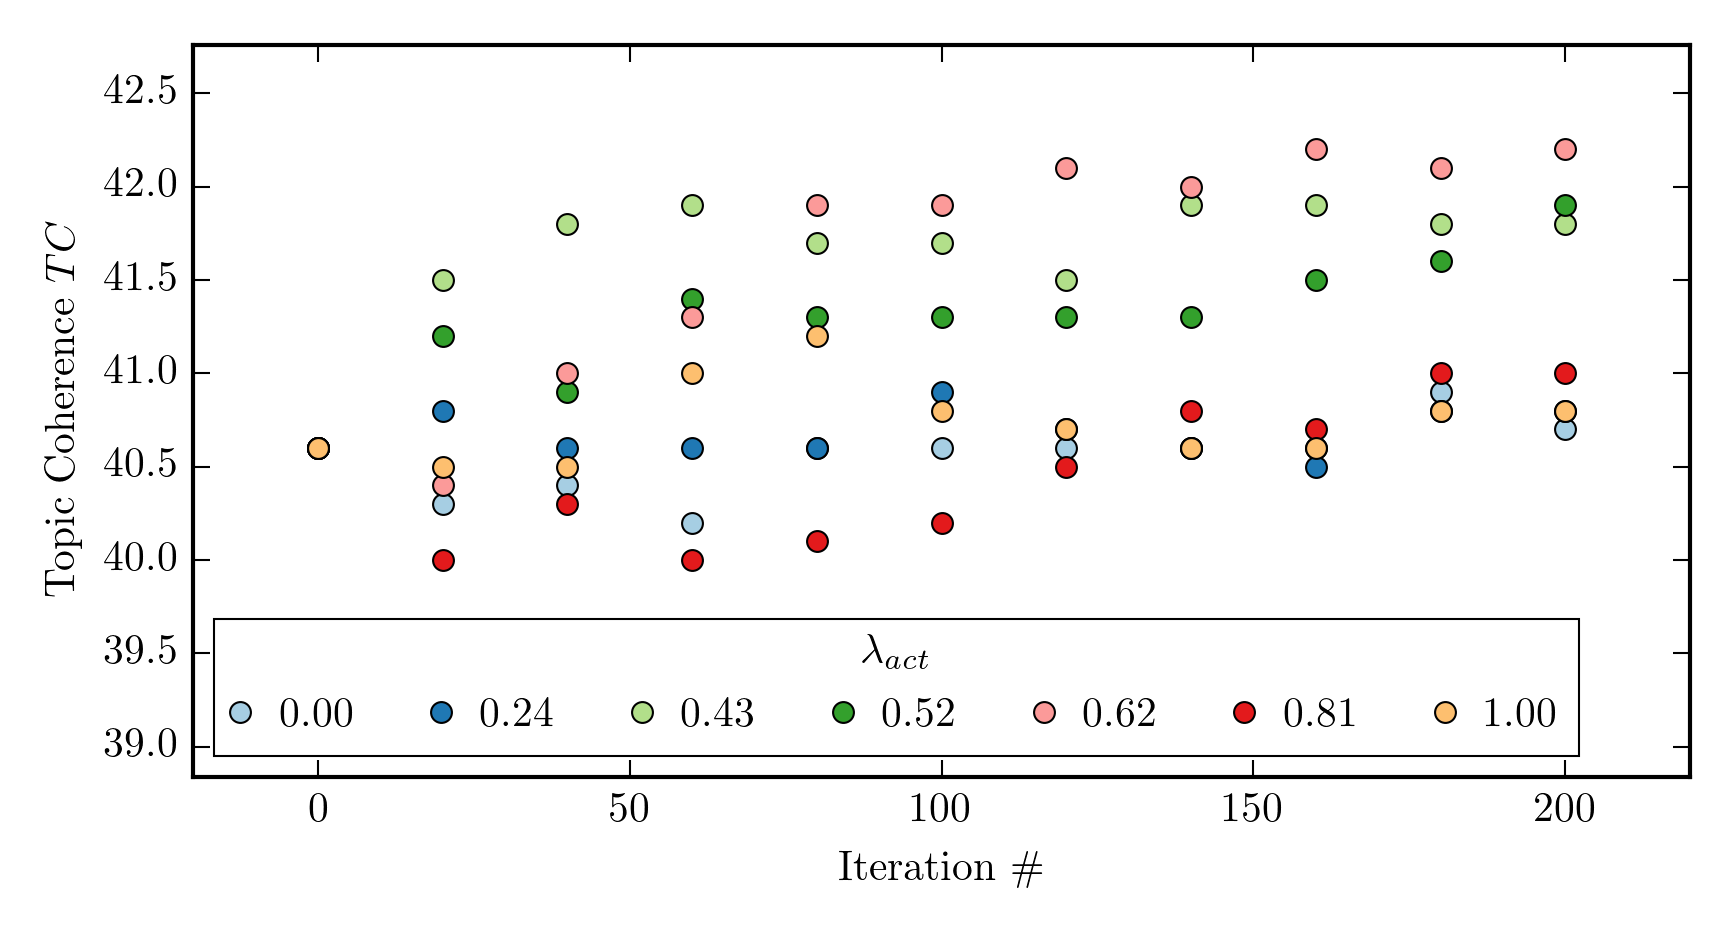
\includegraphics[width=\textwidth]{figures/welda_gaussian_nips_50.png}
         \caption{Topic coherence development for Gaussian WELDA on \textsc{Nips} with corpus-specific embeddings}
         \label{fig:welda_gaussian_nips_50}
  \end{figure}
  \begin{figure}[H]
         \centering
         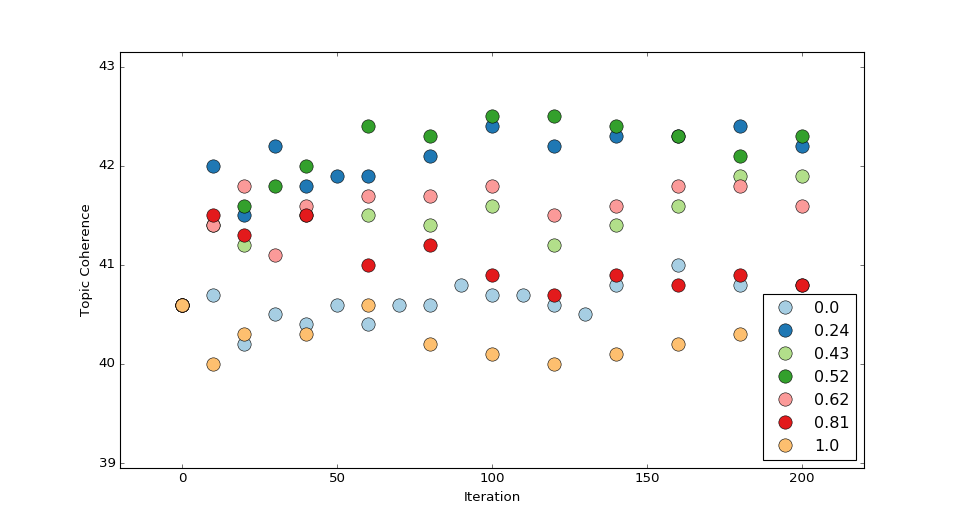
\includegraphics[width=\textwidth]{figures/welda_gaussian_nips_200.png}
         \caption{Topic coherence development for Gaussian WELDA on \textsc{Nips} with Wikipedia as embedding corpus}
         \label{fig:welda_gaussian_nips_200}
  \end{figure}
  
  \subsection{Influence of the parameters $N_{pca}$ and $N_{top}$ on the N{\footnotesize IPS} corpus}
  \label{sec:appendix_welda_gaussian_nips_pca_samples}

  \begin{figure}[H]
         \centering
         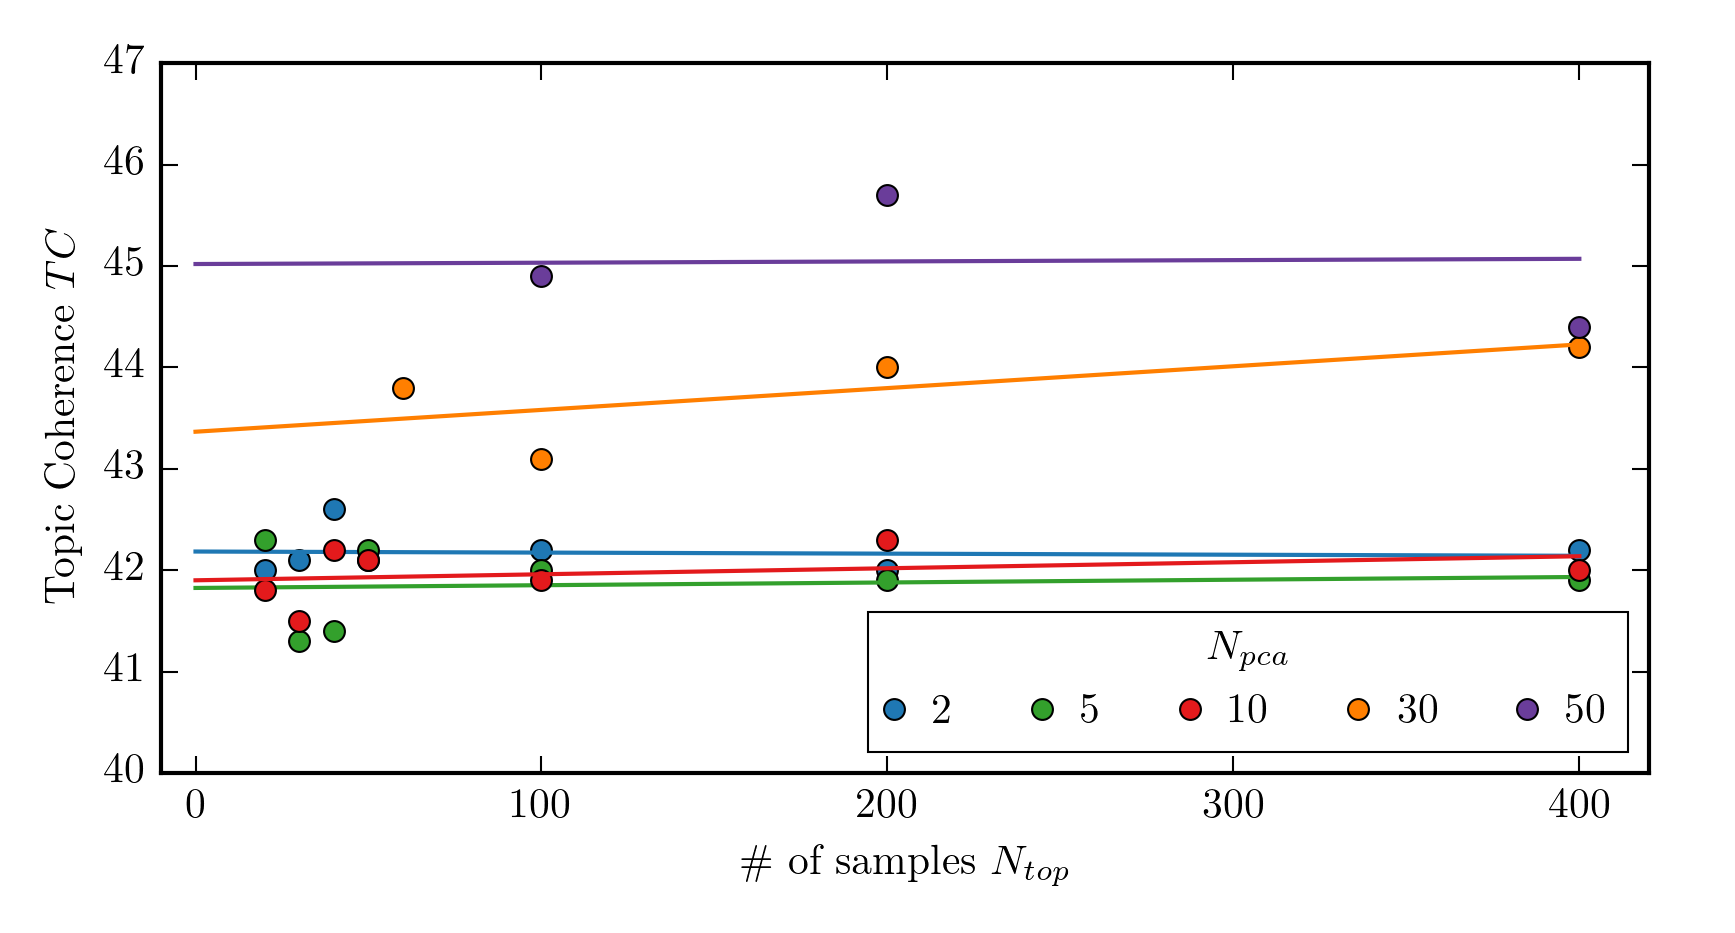
\includegraphics[width=\textwidth]{figures/welda_gaussian_nips_pca_samples.png}
         \caption{Final topic coherence values after 200 iterations for different values of $N_{pca}$ and $N_{top}$ on the \textsc{Nips} corpus. We also plotted a regression line indicating the development for increasing $N_{top}$. The results are similar to the \textsc{20News} corpus: $N_{top}$ has no impact on the topic coherence, $N_{pca}$ has a strong positive correlation. For fixed $N_{top} = 200$, the correlation between $N_{pca}$ and $TC$ is $r_{Pearson} = 0.99$.}
         \label{fig:welda_gaussian_nips_pca_samples}
  \end{figure}

  \subsection{LDA as prerequisite}
  \label{sec:appendix_lda_prerequisite}
  \begin{figure}[H]
         \centering
         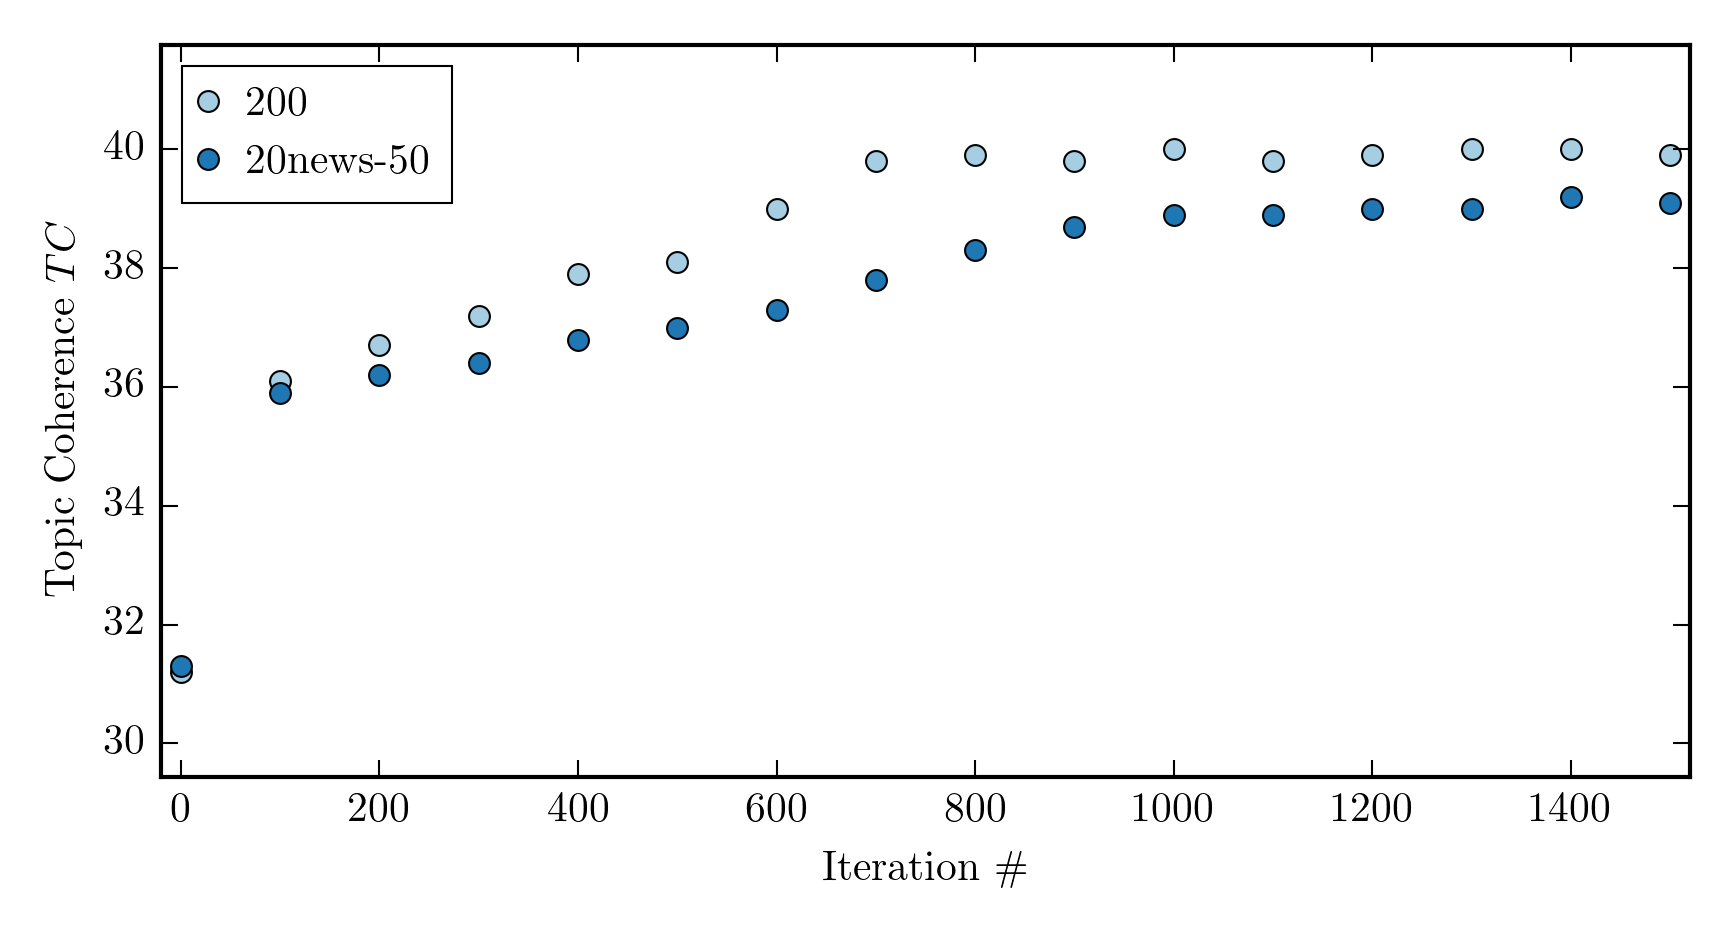
\includegraphics[width=\textwidth]{figures/welda_gaussian_random_init.png}
         \caption{WELDA with $\lambda = 0.5$ and random topic initialization. }
         \label{fig:standard_lda_as_prerequisite}
  \end{figure}

  \subsection{Accuracy of word similarity depending on the number of dimensions in the embedding model}
  \label{sec:embedding_model_dimensions_vs_similarity_corr}
  \begin{figure}[H]
         \centering
         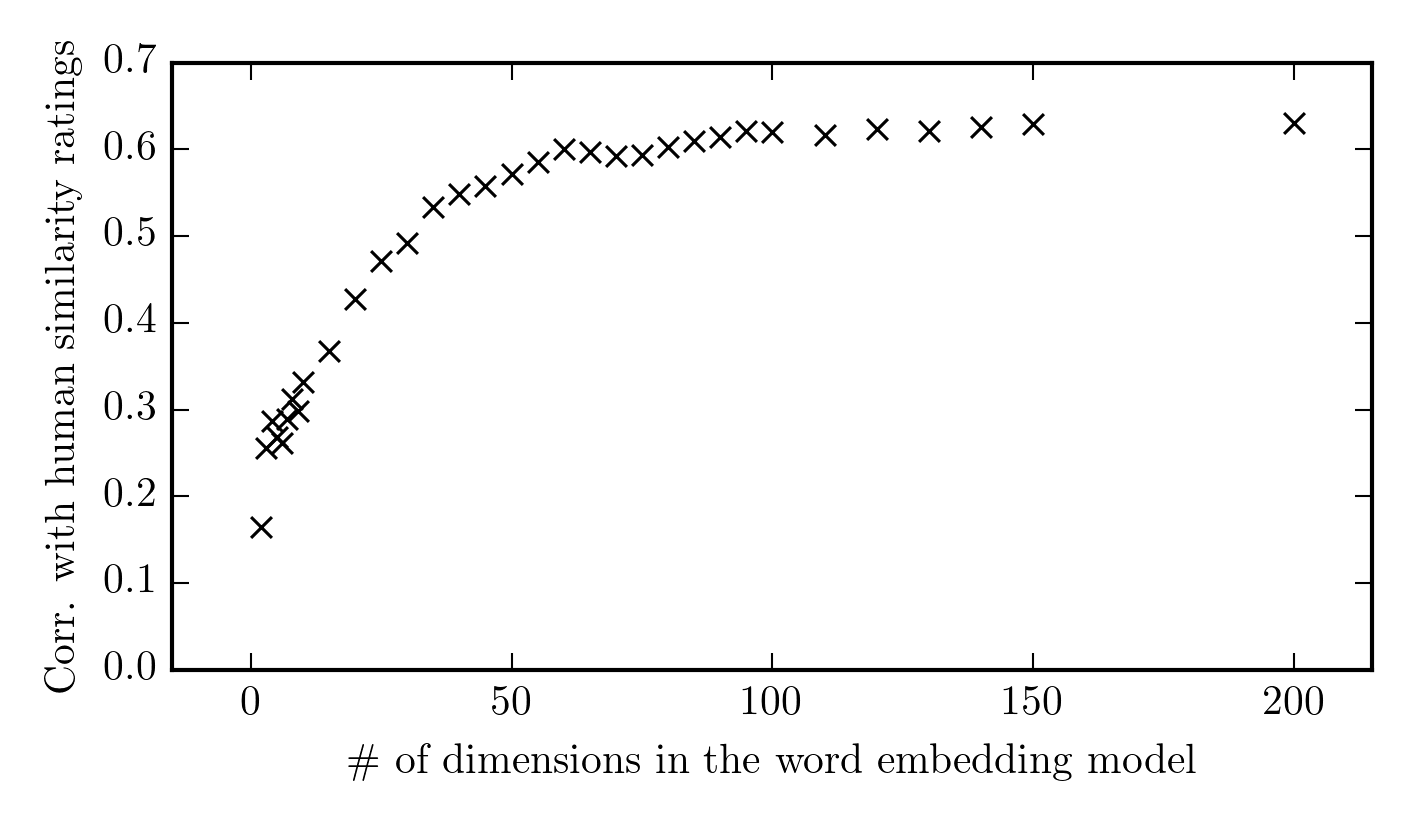
\includegraphics[width=\textwidth]{figures/embedding_model_dimensions_vs_similarity_corr.png}
         \caption{We used the 200-dimensional Wikipedia embeddings and projected them down to fewer dimensions. Then for each dimensionality, we evaluated the correlation with human similarity ratings from the \textsc{WordSim-353}~\cite{Agirre2009} data set. The trend shows, that more dimensions help to capture the word similarity better. Starting at around dimensionality 100, the improvements are only marginal. We use a randomized PCA algorithm, therefore the correlation is not strictly monotonously increasing.}
         \label{fig:embedding_model_dimensions_vs_similarity_corr}
  \end{figure}

  \subsection{WELDA with von Mises-Fisher distributions}
  \label{sec:appendix_welda_vmf}
  \begin{figure}[H]
         \centering
         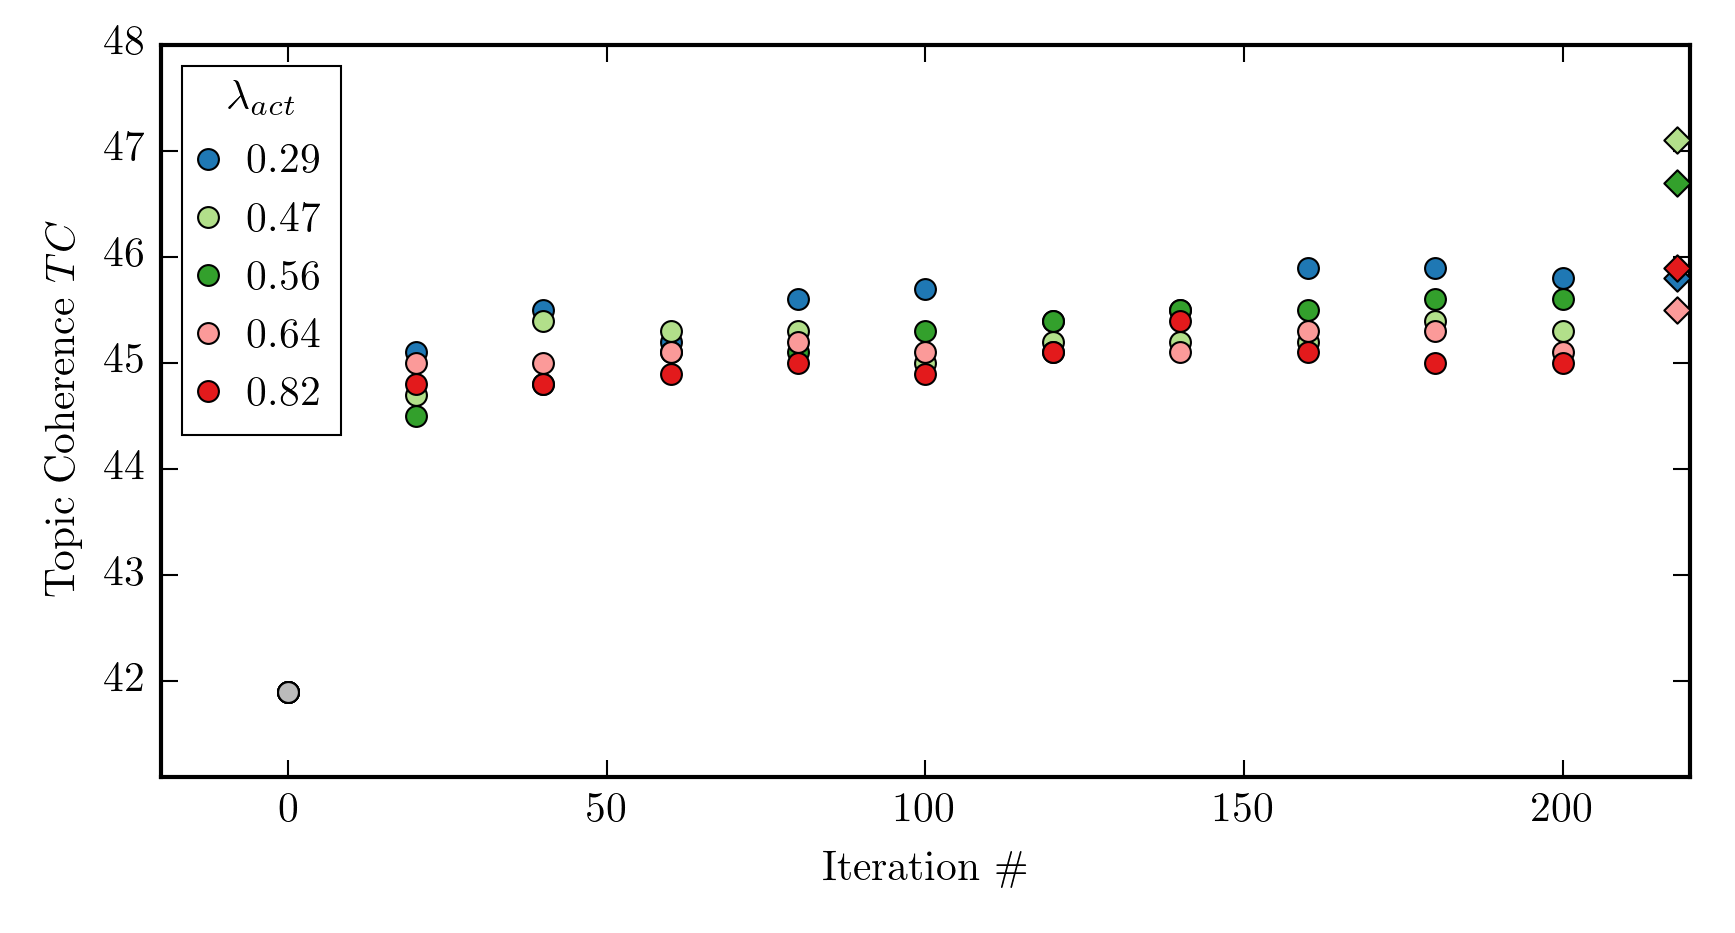
\includegraphics[width=\textwidth]{figures/welda_vmf_20news.png}
         \caption{Von Mises-Fisher WELDA's topic coherence development on \textsc{20News} for different $\lambda_{act}$ values with corpus-specific embeddings. At the end, we plot the respective $TC$ values for Gaussian WELDA, which is superior in this case.}
         \label{fig:welda_vmf_20news}
  \end{figure}

  \section{Comparative Evaluation}
  \subsection{Document classification on 20N{\footnotesize EWS} with corpus-specific embeddings}
  \label{sec:appendix_document_classification_corpus_specific}
  \begin{table}[]
    \ra{1.3}
    \centering
    \caption{Document classification results for the \textsc{20News} corpus when using 50-dimensional embeddings trained on \textsc{20News}.
    All methods are worse than standard LDA.}
    \label{table:document_classification_dim-50}
    \begin{tabular}{lrrrcrrr}
      \toprule
      \multirow{2}{*}{} & \multicolumn{3}{c}{$K = 50$} & \phantom{a} & \multicolumn{3}{c}{$K = 250$} \\ \cmidrule{2-4} \cmidrule{6-8}
                        & $Prec$    & $Rec$     & $F1$     && $Prec$    & $Rec$   & $F1$     \\ \midrule
                        Only Avg. Emb.           & 78.6    & 78.1    & 78.0   && \multicolumn{3}{l}{}        \\
                        LDA                      & 71.1    & 71.2    & 70.1   && 73.2    & 72.8     & 72.6   \\
                        LDA + Avg. Emb.          & 79.1    & 78.6    & 78.5   && 80.3    & 80.1     & 80.0   \\
                        LFTM                     & 69.8    & 68.2    & 67.3   && 73.2    & 72.9     & 72.6   \\
                        LFTM + Avg. Emb.         & \textbf{80.2}    & \textbf{79.9}    & \textbf{79.7}   && \textbf{81.1}    & \textbf{81.5}     & \textbf{81.5}   \\
                        TopicVec                 & 35.1    & 33.0    & 30.6   && 42.1    & 40.1     & 39.7   \\
                        TopicVec + Avg. Emb.     & 78.4    & 78.1    & 78.0   && 78.6    & 78.1     & 78.1   \\
                        WELDA                    & 61.3    & 60.9    & 60.8   && 65.6    & 63.7     & 63.9   \\ % lambda = 0.3
                        WELDA + Avg. Emb.        & 79.2    & 78.6    & 78.3   && 80.4    & 80.1     & 80.1   \\
                        Gaussian LDA             & 53.7    & 54.3    & 52.3   && TODO    & xxxx     & xxxx   \\
                        Gaussian LDA + Avg. Emb. & 77.6    & 76.8    & 76.6   && xxxx    & xxxx     & xxxx   \\
    \bottomrule
    \end{tabular}
  \end{table}

\end{appendices}

\cleardoublepage
\section*{Declaration}
\label{sec:declaration}


I hereby declare in lieu of oath that I composed this thesis independently and without inadmissible help from outside. The sources used are quoted in full and parts that are direct quotations or paraphrases are identified as such.

\vspace{14mm}

Potsdam, December 23rd, 2016

\vspace{20 mm}

Stefan Bunk

% \chapter*{Eigenst\"andigkeitserkl\"arung}

% Hiermit versichere ich, dass ich die vorliegende Masterarbeit selbstst\"andig verfasst sowie keine anderen Quellen und Hilfsmittel als die angegeben verwendet habe.

% \vspace*{1cm}

% Potsdam, der 23. Dezember 2016

% \vspace*{2cm}

% Stefan Bunk



\end{document}
